\documentclass[oneside,12t]{classes/Thesis}

\usepackage[utf8]{inputenc}
\usepackage{ulem}
\usepackage[english]{babel}

\usepackage{url}
\graphicspath{{img/}}
\DeclareGraphicsExtensions{.pdf,.png}

\usepackage[T1]{fontenc}
\usepackage{pslatex}

\usepackage{fixltx2e}


\usepackage[french,onelanguage,ruled]{algorithm2e}
%\usepackage{algorithmic}
\usepackage{caption}
\usepackage{subfigure}

\usepackage{color}
\usepackage{listingsutf8}

%listings}

\definecolor{cppred}{rgb}{0.6,0,0} % for strings
\definecolor{cppgreen}{rgb}{0.25,0.5,0.35} % comments
\definecolor{cpppurple}{rgb}{0.5,0,0.35} % keywords
\definecolor{cppblue}{rgb}{0.25,0.35,0.75} % javadoc

\lstset{
  language=C++,
  numbers=left,
  numberstyle=\footnotesize,
  stepnumber=1,
  backgroundcolor=\color{white},
  identifierstyle=\color{cpppurple},
  keywordstyle=\bfseries,
  stringstyle=\color{cppred},
  commentstyle=\color{cppgreen},
  showspaces=false,
  showstringspaces=false,
  showtabs=false,
  frame=single,
  tabsize=2,
  captionpos=b,
  breaklines=true,
  breakatwhitespace=false,
  escapeinside={\%*}{*)}
}





\title{Un modèle de programmation à grain fin pour la parallélisation de solveurs linéaire creux}


\authorFirstName{Corentin}
\authorLastName{Rossignon}
\authorMail{corentin.rossignon@gmail.com}

\directors{Raymond \textsc{Namyst}}
\codirectors{Olivier \textsc{Aumage} et Samuel \textsc{Thibault}}
\responsables{Pascal \textsc{H\'{e}non}}

\laboratory{LaBRI}
\laboratoryURL{http://www.labri.fr/}
\university{Université de Bordeaux}
\universityURL{http://www.univ-bordeaux.fr/}


\logo{bordeaux1}
\degreeDate{?? ???? 2015}
\degree{Docteur de l'université de Bordeaux}
\degreeSpeciality{Informatique}

\metadataSetup

% turn of those nasty overfull and underfull hboxes
\hbadness=10000
\hfuzz=50pt

\begin{document}

\dominitoc
\tikzstyle{decision} = [diamond, draw, fill=blue!20,
text width=3em, text centered, node distance=2.5cm, inner sep=0pt,font=\scriptsize]
\tikzstyle{block} = [rectangle, draw, fill=blue!20,
text width=4em, text centered, rounded corners, minimum height=1em,font=\scriptsize]
\tikzstyle{line} = [draw, thick, color=black!50,font=\scriptsize]
\tikzstyle{cloud} = [draw, ellipse,fill=red!20, node distance=2.5cm,
minimum height=0.1em,font=\scriptsize]

\maketitle

%set the number of sectioning levels that get number and appear in the contents
\setcounter{secnumdepth}{3}
\setcounter{tocdepth}{3}

\frontmatter % book mode only
\pagenumbering{roman}
%Test

%La résolution de grands systèmes linéaire creux est un élément essentiel des simulations numériques. Ces résolutions peuvent représenter jusqu'à 80\% du temps de calcul des simulations.
Une parallélisation efficace des noyaux d'algèbre linéaire creuse conduira donc à obtenir de meilleurs performances. En mémoire distribuée, la parallélisation de ces noyaux se fait le plus souvent en modifiant le schéma numérique. Par contre, en mémoire partagée, un parallélisme plus efficace peut être utilisé. Il est donc important d'utiliser deux niveaux de parallélisme, un premier niveau entre les noeuds d'une grappe de serveur et une deuxième niveau à l'intérieur du noeud. Lors de l'utilisation de méthodes itératives en mémoire partagée, les graphes de tâches permettent de décrire naturellement le parallélisme en prenant comme granularité le travail sur une ligne de la matrice. Malheureusement, cette granularité est trop fine et ne permet pas d'obtenir de bonnes performances.
Dans cette thèse, nous allons étudier le problème de la granularité pour la parallélisation par graphe de tâches. Nous proposerons d'augmenter la granularité des tâches de calcul en créant des agrégats de tâches qui deviendront eux-mêmes des tâches. L'ensemble de ces agrégats et des nouvelles dépendances entre les agrégats formera un graphe de granularité plus grossière. Ce graphe sera ensuite utilisé par un ordonnanceur de tâches pour obtenir de meilleurs résultats. Nous utiliserons comme exemple la factorisation ILU d'une matrice et nous montrerons les améliorations apportées par cette méthode. Dans un second temps, nous nous concentrerons sur les machines à architecture NUMA. Dans le cas de l'utilisation d'algorithmes limités par la bande passante mémoire, il est intéressant de réduire les effets NUMA liés à cette architecture. Nous montrerons comment prendre en compte ces effets dans un intergiciel à base de tâches pour améliorer les performances d'un programme.

Mots-clés : parallélisme, graphe de tâches, supports d’exécution, NUMA, multi-coeurs, algèbre linéaire creuse

%With the commoditization of multi-core processors in clusters, the inter-node parallelism expressed by HPC applications needs to be complemented by a finer-grained parallelism that takes advantage of shared memory at the intra-node level.
%
The fine grain parallelism means that we can exhibit new levels of parallelism by parallelizing some operations that are usually done sequentially.
%
Usually it consists in parallelizing some algorithms performed inside a MPI process by using several cores of a cluster node.
%
Indeed, by taking advantage of the shared memory at the node level, some algorithms are then parallelizable, whereas they could not be efficiently parallelized using the static partitioning of data and communication overhead imposed by a distributed memory framework (e.g., MPI).


Some popular shared memory parallel frameworks like Intel TBB~\cite{Intel::TBB},
Cilk~\cite{cilk} or OpenMP 3.0~\cite{openmp08} propose programming models that
considerably alleviate the fine grain parallelization in a shared memory environment.
Those models rely on the use of a scheduler that dispatches the computation tasks
at runtime on the available cores of a cluster node. The simplest form of fine grain
parallelism consists in splitting independent works done in a loop among the cores.
More complex algorithms require to expose the parallelism as an Direct Acyclic Graph (DAG)
where each node is a task that consists in a group of operations that
can only be computed once all its predecessor tasks have also been completed.
With such a computational task graph approach, the work that belongs to the developer
is to describe the computations as a collection of tasks and to give  the set of
predecessor and successor tasks for each of them. The runtime scheduler is then
in charge of launching tasks on the hardware and achieve a good load-balancing.

Nevertheless, these programming models lack some features to handle efficiently
some important classes of problems.
Indeed, very often two crucial problems have to be addressed in order to achieve
an efficient fine grain parallelization:
\begin{itemize}
\item The first one is to obtain a correct task grain size for a good parallel
  efficiency: A too fine parallelism grain leads to bad performances caused by
  the task management and scheduling overhead, while a too coarse grain does not
  provide enough parallelism for the hardware capability and causes load balancing issues.
\item The second problem is to take into account the Non Uniform Memory Accesses (NUMA)
  that are caused by the time penalty when a core needs to access some data that
  are not physically located on a memory bank directly linked to its socket.
  Therefore, the physical location of memory allocation needs to be carefully driven
  to match the task scheduler policy in order to minimize these time penalties.
\end{itemize}

In this paper, we present some solutions to address these two problems at the
level of the programming model.
Our main motivation is that we want a programming model that adds as few
programming effort as possible beyond a natural task based parallelization of
an algorithm (using TBB for example) to obtain a better efficiency by taking
care of NUMA and task grain size.

%%  To reach this goal, in the first place we have enhanced the C++ programming interface proposed by Intel TBB to
%%   add some coarsening operators based on the task description of a problem. To that end we have implemented a task aggregation library that does
%%   the coarsening graph operations using different heuristics that can be selected and combined by the user using a simple string parameter.
%%  % It is important to note that the default aggregation operator when merging two task consists in sequentially calling the function of each task in the coarse task
%%  % but a developer can also overload the aggregate operator of the task class to redefine how to merge two tasks; for example instead of calling sequentially each task function
%% %The coarsen graph obtained can then be used on top of any runtime scheduler: our implementation interface allow to use TBB, OpenMP or our own NUMA-aware scheduler
%%   %in a seamless manner; we can switch between runtime systems by simply adding a flag at compilation.
%%   We have interfaced this library with several runtimes (Intel TBB, OpenMP and also our own implementation of a runtime scheduler) that can execute the coarse task graph obtained after this steps.
%%   The second part of the work was to take care of NUMA effects. Our approach has been to provide some special allocators to the user so that

%To evaluate the benefit of our work we present some experiments on the
%parallelization of an iterative solver for sparse linear systems. A popular
%approach to solve large sparse linear systems of equations is a Krylov
%method (such as GMRES or Conjugate Gradient) preconditioned by an incomplete
%factorization (see~\cite{Saad96IMSLS}).
%This is often the most time consuming part of a numerical simulation.
%The usual way to parallelize this kind of solvers is to use a weaker form of
%the preconditioner in parallel by preconditioning subdiagonal blocks of the
%matrix: The subdiagonal blocks are usually obtained thank to a partition of
%the adjacency graph of the matrix.
%Outside the preconditioner, the operations required in a Krylov method are
%vector operations (mostly BLAS1 type like dot products or AXPY) and matrix % CR: CHECK: replace `,' by or
%vector products. Those operations are naturally dealt with parallel loop
%splitting  (e.g., {\em parallel for} in OpenMP).
%In this paper, we have chosen to focus on the fine grain parallelization of
%the ILU preconditioner.
%In this case, more levels of parallelism can be obtained because the factorization
%and triangular solves of a submatrix can be parallelized on several cores.
%Incomplete factorization and associated triangular solve of a sparse matrix
%is a problem that is well representative of the difficulty that one can encounter
%with fine-grain parallelization: The fine grain description of these algorithms
%is natural. However, in practice a straight task based parallelization using TBB or
%OpenMP does not deliver good speed-ups because of the very low computational cost of
%a task and the NUMA effect when accessing the coefficients of the matrix and vector.
%In the experiment results, we will evaluate our programming model on those algorithms.

%%   In a Krylov method the operation needed are vector operations (dot product, AXPY as define by BLAS1..) and matrix vector multiplications (the matrix
%%   is usually really sparse). The most complicated part for a fine grain parallelization
%%   We have specifically studied the parallelization of an incomplete LU factorization () and the triangular solves associated.

%%   LU
%%   (ILU(k)) factorization. The ILU factorization is a very popular preconditioner for Krylov met
%%   A very popular approach to solve linear system is a Krylov method like GMRES

%%   To handle the task grain problem our approach is to coarsen the fine-grained parallelism through
%%   general heuristics of graph coarsening based on the task graph description of the user. The originality
%%   of our approach is to alleviate the programming task by letting the developer express the natural task decomposition of its problem
%%   but then propose a simple operator of coarsening that will apply some heuristics to produce a coarsest task graph.

%%   application programmer first expresses the fine parallelism sparse
%%   linear algebra parallelism in a natural way. Then, our coarsening
%%   mechanism applies a selectable coarsening scheme to aggregate
%%   individual tasks as larger task groups, so as to efficiently feed the
%%   platform computing units.



%%   Sparse linear solvers are often the main computational bottleneck in numerical simulations; a large class of the iterative method are composed
%%   of a Krylov method preconditioned by an Incomplete LU (ILU) factorization (see for example).

%% %%   For sparse linear algebra computations, it is common to use domain
%% %%   decomposition to generate parallelism. In the special case of
%% %%   iterative methods, however, domain decomposition may impact the
%% %%   numerical stability and thus the number of steps required for reaching
%% %%   convergence. Moreover, the natural parallelism at the sparse linear
%% %%   algebra computation is too fine grained.

\tableofcontents
\mtcaddchapter
\mainmatter % book mode only



%=========================================================
\chapter{Contexte : simuler l'extraction du pétrole}
\minitoc
\vspace{1cm}
%=========================================================

%+++++++++++++++++++++++++++++++
\section{La simulation de réservoir}
%-------------------------------
\subsection{Vue d'ensemble}
Dans les profondeurs de la Terre, du pétrole et du gaz naturel se trouvent piégés.
%
Ces sources d'énergie sont le résultat de la transformation de matière organique, provenant de végétaux et d'animaux morts, sous très fortes contraintes durant des millions d'années.
%
Les compagnies pétrolières telles que Total ont pour but de localiser et d'optimiser l'extraction de ces ressources.

Plus généralement, nous appelons réservoir d'hydrocarbure, ou simplement réservoir, une concentration majeure de pétrole et/ou de gaz naturel sous le sol.
%
La première étape pour trouver un réservoir consiste à analyser le sous-sol avec des ondes acoustiques.
%
Ces ondes sont générées par des explosions pour les analyses sous la mer ou avec un camion sismique pour la surface de la Terre.
%
Ces ondes sont ensuite analysées avec des logiciels de modélisation basés sur les équations des ondes, les compagnies pétrolières peuvent ainsi obtenir une bonne représentation du sous-sol.
%
Après analyse de cette représentation, des puits d'explorations sont forés pour s'assurer de la présence de pétrole.
%
Quand un réservoir est trouvé, l'une des premières questions est : ``Est-il rentable d'exploiter ce réservoir ?''.
%
La simulation de réservoir est un des outils permettant de répondre à cette question.
%
En faisant une simulation de fluides en milieu poreux, les compagnies pétrolières peuvent obtenir une approximation de la quantité d'huile pouvant être récupérée.
%
Si l'exploitation du réservoir est rentable, les compagnies pétrolières commencent l'exploitation.

Mais il ne suffit pas de creuser et d'attendre que le pétrole jaillisse sous la forme d'un geyser comme nous pouvons le voir dans certains cartoons.
%
Les compagnies pétrolières doivent installer des puits.
%
Les puits peuvent être catégorisés en deux catégories majeures (Fig.~\ref{fig:wells}) :
%
\begin{itemize}
  \item les puits injecteurs, ce sont les puits qui augmentent la pression à l'intérieur du réservoir en injectant de la matière (eau, gaz(CO$_2$), polymère ...);
  \item les puits producteurs, ce sont les puits qui récupèrent l'huile, ils sont aussi essentiels au contrôle de la pression en produisant plus ou moins d'huile et de gaz.
\end{itemize}
%   (-_-)   %
\begin{figure}[!h]
  \centering
  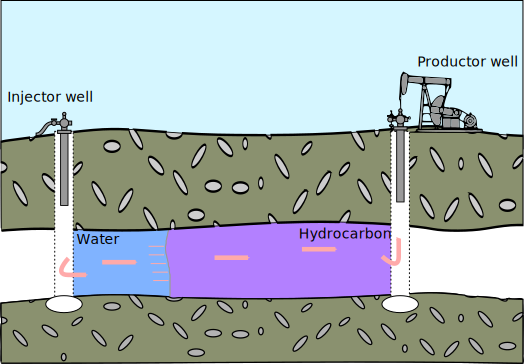
\includegraphics[width=0.8\textwidth]{wells}
  \caption{Exemple d'un champ avec deux puits.}
\label{fig:wells}
\end{figure}

L'une des activités des ingénieurs réservoir consiste à trouver le nombre optimal de puits ainsi que l'emplacement optimal de chacun pour exploiter le réservoir.
%
Encore une fois, la simulation de réservoir leur permet de tester différentes configurations de placement des puits.
%
Plus tard, quand la compagnie pétrolière commence à exploiter le champ, il est intéressant d'avoir des prévisions sur la production d'huile.
%
Une fois de plus, ces résultats sont obtenus avec une simulation de réservoir (Fig.~\ref{fig:floviz}).

%   (-_-)   %
\begin{figure}[!h]
  \centering
  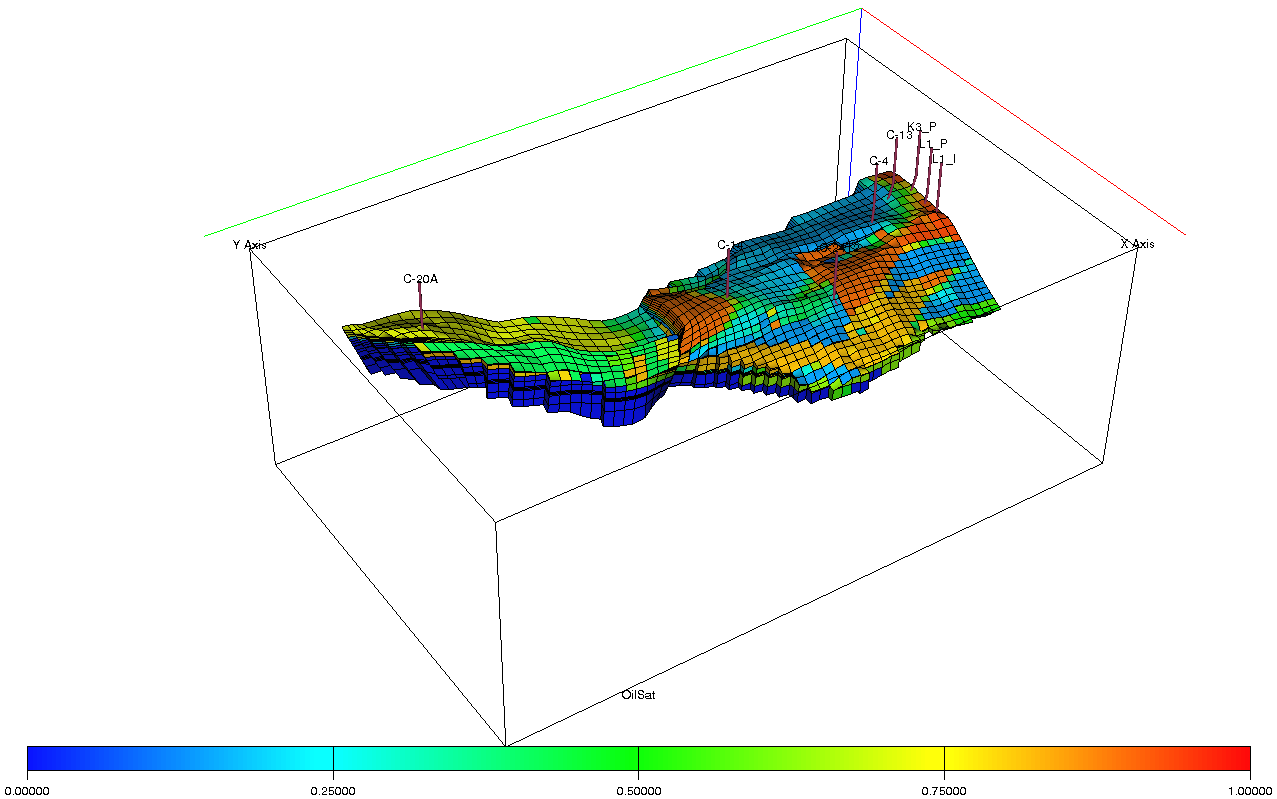
\includegraphics[width=\textwidth]{reservoir}
  \caption{Visualisation de la quantité d'huile dans le réservoir, l'image provient du logiciel floviz.}
\label{fig:floviz}
\end{figure}




Comme montré précédemment, la simulation de réservoir est une étape clé dans le processus de récupération d'hydrocarbures.
%
Il est intéressant pour une compagnie pétrolière de simuler de plus en plus précisément l'intérieur d'un réservoir et bien sûr le simuler aussi vite que possible.
%
Focalisons-nous sur la structure interne d'un simulateur de réservoir.

%-------------------------------
\subsection{De la physique au calcul informatique}
Pour pouvoir faire une simulation de réservoir, on démarre avec un physicien qui modélise un écoulement de fluide en milieu poreux.
%
La plupart de ces modèles sont basés sur trois équations physiques : la conservation de la masse, la loi des gaz parfaits et la loi de Darcy.
%
Puis le réservoir est discrétisé en cellules en utilisant la méthode des volumes finis.
%
Pour chaque cellule du réservoir, nous obtenons une équation non-linéaire par variables primaires (e.g. : pression, saturation en huile, ...).
%
Pour résoudre le système d'équations non-linéaires nous utilisons la méthode Newton–Raphson.
%
Cette méthode est itérative, nous démarrons avec une valeur initiale $X_0$ suffisamment proche de la solution $X_n$ qui satisfait $F(X_n) = 0$.
%
La méthode Newton–Raphson nous garantit que chaque itération nous rapproche du minimum local.

%   (-_-)   %
\begin{figure}[!ht]
  \centering
  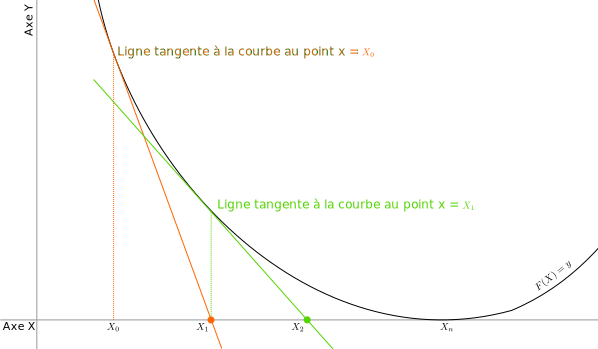
\includegraphics[width=0.8\textwidth]{newton}
  \caption{Exemple de deux étapes de Newton in une dimension.
    Chaque tangente corresponde à une équation linéaire à résoudre.
    Nous recherchons $X_n$ et nous démarrons au point $X_0$.}
\label{fig:newton}
\end{figure}

L'exemple de la figure~\ref{fig:newton} n'est que dans une seule dimension, mais la même approche peut être utilisée quand on travaille avec un nombre arbitraire de dimensions.
%
Les équations linéaires de la simulation de réservoir peuvent être représentées sous la forme d'une matrice creuse très grande.
%
Dans cette matrice, chaque ligne représente les interactions des éléments d'une cellule avec les éléments de son voisinage direct.
%
Donc, si nous prenons un cube 3D régulier, nous pouvons avoir jusqu'à sept interactions par lignes.
%
Chaque interaction est représentée sous la forme d'une petite matrice dense dont la taille correspond au nombre de variables primaires.
%
Par la suite, un solveur de systèmes d'algèbre linéaire creux est utilisé.
%
Pour la simulation de réservoir, nous utilisons un GMRES préconditionné parce que nos matrices ne sont pas symétriques.

%-------------------------------
\subsection{Simulation d'un exemple physique simple}
Prenons un exemple physique simple pour avoir une idée de comment l'algèbre linéaire peut être utilisée dans une simulation.
%
Cet exemple est trivial et peut être résolu directement sans utiliser l'algèbre linéaire mais il permet de comprendre facilement l'utilisation de l'algèbre linéaire dans un code de simulation numérique.
%
Nous souhaitons simuler une colonne remplie d'huile.
%
Nous connaissons la densité de l'huile contenue dans la colonne : $\rho = 0.9192~kg/m^3$.
%
Nous connaissons aussi l'équation physique de la pression hydrostatique :
%
\begin{equation}
\label{eq:hydrostatic}
\frac{\mathrm d P}{\mathrm d z} = \rho{}g
\end{equation}
%
Dans l'équation~\eqref{eq:hydrostatic}, $P$ désigne la pression, $z$ la profondeur et $g$ l'accélération gravitationnelle.
%
En utilisant le théorème de Taylor au premier ordre, nous obtenons l'équation :
%
\begin{equation}
P(z_0+h) = P(z_0) + h \frac{\mathrm d P}{\mathrm d z} (z_0) + o(h^2)
\end{equation}
\begin{equation}
\frac{\mathrm d P}{\mathrm d z} (z_0) = \frac{P(z_0+h) - P(z_0)}{h} + o(h^2)
\end{equation}

%   (-_-)   %
\begin{figure}[!h]
  \centering
  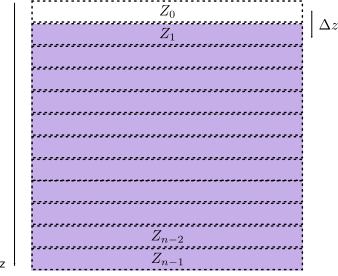
\includegraphics[width=0.5\textwidth]{oil_column}
  \caption{Schéma de la colonne d'huile, il s'agit d'une discrétisation en $n$ cellules et le centre de chaque cellule est séparé d'une distance $\Delta{z}$.}
  \label{fig:oil_schema}
\end{figure}
%
On discrétise le problème en $n$ cellules avec la méthode des différences finies (Fig.~\ref{fig:oil_schema}) : considérons $Z_i$ l'approximation de $z$ sur la cellule $i$, $i$ allant de $0$ à $n-1$.
%
Chaque cellule est séparée d'une distance $h$ appelée $\Delta{z}$ :
%
\begin{equation}
\label{eq:taylor_fd}
\frac{\mathrm d P}{\mathrm d z}(Z_i) \approx \frac{P(Z_{i}) - P(Z_{i-1})}{\Delta{z}}
\end{equation}
%
L'injection de \eqref{eq:taylor_fd} dans \eqref{eq:hydrostatic} conduit à :
%
\begin{equation}
\frac{P(Z_{i}) - P(Z_{i-1})}{\Delta{z}} = \rho{}g
\end{equation}
\begin{equation}
\label{eq:system_pressure}
P(Z_{i}) - P(Z_{i-1}) = \rho{}g\Delta{z}
\end{equation}
Nous avons aussi la condition limite qu'à la profondeur 0, la pression est de 1000~hPa ou $10^5$~Pa:
%
\begin{equation}
P(Z_0) = 10^5
\end{equation}
%
Nous pouvons donc écrire le système entier sous la forme d'une matrice à $n$ lignes :
%
\begin{equation}
\label{eq:ax_b}
\begin{bmatrix}
   1   &    0   &    0   & \cdots & \cdots & \cdots & \cdots &   0    \\
  -1   &    1   &    0   & \ddots &        &        &        & \vdots \\
   0   &   -1   &    1   &    0   & \ddots &        &        & \vdots \\
\vdots & \ddots & \ddots & \ddots & \ddots & \ddots &        & \vdots \\
\vdots &        & \ddots & \ddots & \ddots & \ddots & \ddots & \vdots \\
\vdots &        &        & \ddots &   -1   &    1   &    0   &   0    \\
\vdots &        &        &        & \ddots &   -1   &    1   &   0    \\
   0   & \cdots & \cdots & \cdots & \cdots &    0   &   -1   &   1    \\
\end{bmatrix}
\begin{pmatrix}
  P(Z_0)  \\
  P(Z_1)  \\
\vdots \\
\vdots \\
\vdots \\
\vdots \\
P(Z_{n-2}) \\
  P(Z_{n-1})  \\
\end{pmatrix}
=
\begin{pmatrix}
 10^5  \\
\rho{}g\Delta{z}     \\
\vdots \\
\vdots \\
\vdots \\
\vdots \\
\rho{}g\Delta{z} \\
\rho{}g\Delta{z}    \\
\end{pmatrix}
\end{equation}
En multipliant de chaque ligne de $A$ par $x$, nous obtenons exactement le système d'équations \eqref{eq:system_pressure}.
%
Ce système d'équation dont la forme générale est $A.x=b$ (où $A$ est une matrice inversible, $b$ un vecteur donné et $x$ le vecteur des inconnues que l'on cherche à déterminer), est la partie critique en temps CPU dans beaucoup de code de simulation numérique.

%+++++++++++++++++++++++++++++++


%+++++++++++++++++++++++++++++++
\section{Algèbre linéaire}
%-------------------------------
\subsection{Algèbre linéaire dense}
Résoudre un système d'équations linéaire équivaut à résoudre un problème du type $Ax=b$ dans lequel $A$ est une matrice, $b$ est le vecteur second membre du système et $x$ est le vecteur que nous cherchons.
%
Dans l'exemple de la simulation de colonne d'huile, nous avons une matrice triangulaire pour $A$, la solution peut donc être trouvée directement en résolvant chaque équation une à une en démarrant par $P(X_0) = 1000$.
%
Mais ce n'est pas toujours aussi facile.
%
Dans des cas plus difficiles, d'autres méthodes doivent être utilisées comme l'élimination de Gauss-Jordan, l'élimination de variables ou bien la décomposition LU.


En informatique, il existe plusieurs bibliothèques spécialisées dans les opérations d'algèbre linéaire dense.
%
La plus connue est BLAS\footnote{Basic Linear Algebra Subprograms}, c'est un ensemble d'opérations d'algèbre linéaire qui s'appliquent sur des vecteurs et des matrices.
%
Ces opérations sont classées en 3 niveaux :
\begin{itemize}
  \item Niveau 1 : ce sont les opérations sur les vecteurs (produit scalaire, addition de deux vecteurs, ...);
  \item Niveau 2 : ce sont les opérations matrice-vecteur (multiplier une matrice par un vecteur, résoudre un système d'équations linéaires dont les coefficients sont dans une matrice triangulaire, ...);
  \item Niveau 3 : ce sont les opérations matrice-matrice (multiplier une matrice par une autre matrice, ...).
\end{itemize}
%
Le niveau des BLAS est directement lié à leur complexité en nombre d'opérations.
%
Les BLAS de niveau 1 sont limités par la bande passante mémoire, il n'y a aucune réutilisation des données.
%
Chaque donnée n'est utilisée qu'une seule fois, la seule optimisation possible se fait au niveau du prefetch mémoire.
%
Les BLAS de niveau 2 peuvent réutiliser des données du vecteur, des optimisations peuvent être effectuées ici, par exemple il est possible de garder des parties du vecteur en cache.
%
Les BLAS de niveau 3 ont une complexité plus grande ce qui permet d'avoir un plus grand nombre d'optimisations~\cite{blas3_opt}.

LAPACK\footnote{Linear Algebra PACKage} est une autre bibliothèque utilisée en algèbre linéaire, elle est construite par dessus BLAS.
%
Les opérations faites dans BLAS et LAPACK sont bien optimisées, par exemple certaines implémentations utilisent la structuration en bloc qui permet d'optimiser la localité des données et de réduire les défauts de cache.
%
D'autres implémentations utilisent les instructions SIMD(SSE, AVX, ...) des processeurs modernes~\cite{intel_mkl}.
%
Des implémentations GPGPU\footnote{Genenal Purpose Graphical Processing Unit}~\cite{nvidia_cublas} existent aussi, de même que des implémentations en mémoire distribuée~\cite{dplasma}.
%
La plupart de ces optimisations peuvent exister parce que le motif des accès mémoires des opérations du type BLAS est déterministe et que certaines opérations peuvent être réordonnées sans impacter le résultat final.


Retournons à la matrice de l'équation~\eqref{eq:ax_b}, nous pouvons voir que cette matrice contient énormément de valeurs nulles et que ces valeurs n'ont aucun impact sur le calcul.
%
On peut différencier les matrices avec beaucoup de valeurs nulles, des matrices avec une majorité de valeurs non nulles.
%
Une matrice peut être considérée creuse quand son nombre de valeurs non nulles est de l'ordre de la dimension de la matrice.
%
Les méthodes utilisées pour résoudre les systèmes linéaires creux sont différentes de celles utilisées pour les systèmes linéaires denses.

%-------------------------------
\subsection{Algèbre linéaire creuse}
A la différence de l'algèbre linéaire dense, la majorité des calculs fait en creux sont irrégulier.
%
C'est en partie dû à la façon de stocker la matrice creux.
%
En effet, pour avoir un stockage efficace, seul les coefficients non nuls de la matrice creuse sont stockés.
%
Le motif des valeurs non nuls de la matrice est définit par le problème que nous souhaitons résoudre.
%
Le format le plus générique pour stocker des matrices creuses s'appelle COO (fig.~\ref{fig:COO}).
%
Dans ce format, chaque valeur non nuls est stocké avec ses coordonnées 2D dans la matrice.
%
Une autre format, lui aussi générique, est souvent utilisé, il s'agit du format CSR\footnote{Compress Sparse Row} (fig.~\ref{fig:CSR}).
%
Les éléments non nuls sont triés par ligne puis le tableau {\em PTR} du format de stockage nous permet de retrouver la ligne d'un élément.
%
D'autre formats moins générique existent mais nous n'en parlerons pas ici.

\begin{figure}[!ht]
     \begin{center}
        \subfigure[Exemple de matrice creuse]{%
            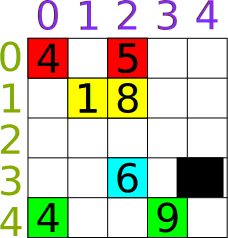
\includegraphics[width=0.25\textwidth]{matrix_format}
        }%
        \subfigure[Stockage COO]{%
           \label{fig:COO}
           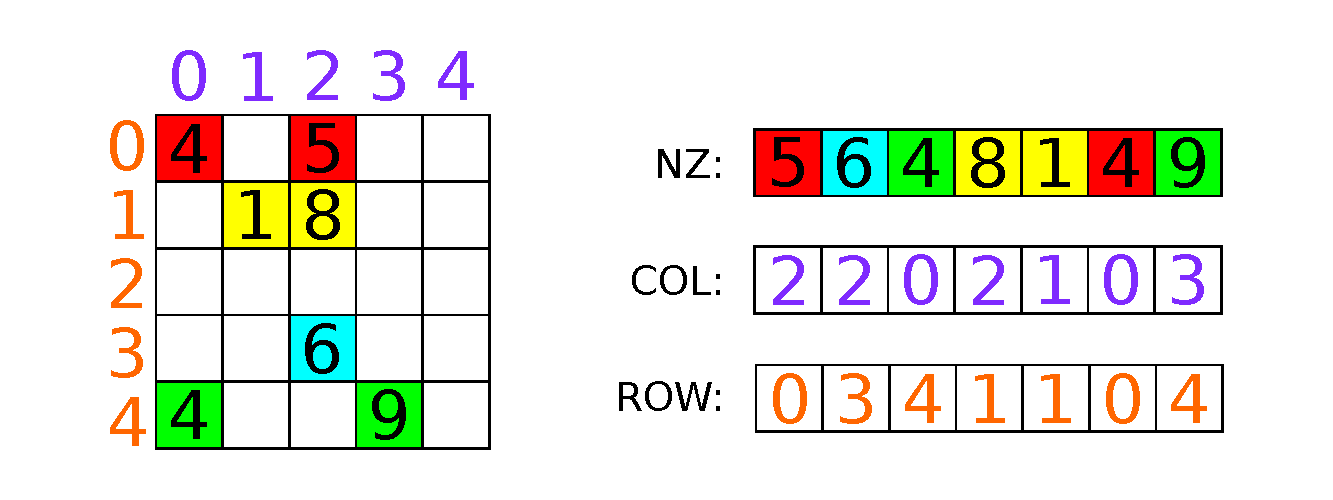
\includegraphics[width=0.35\textwidth]{COO}
        }%
        \subfigure[Stockage CSR]{%
            \label{fig:CSR}
            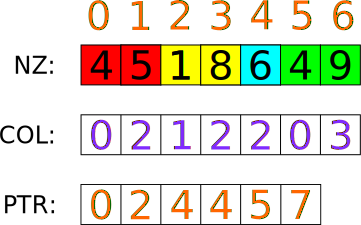
\includegraphics[width=0.35\textwidth]{CSR}
        }%
    \end{center}
    \caption{Comparaison entre les formats de stockage de matrices creuses COO and CSR.}
    \label{fig:matrix_storage}
\end{figure}

Le choix du format de stockage va avoir beaucoup d'effet sur les performances d'une application.
%
Avec la plupart des format, nous aurons au moins deux accès mémoire pour obtenir les coordonnée 2D d'un coefficient non nul alors qu'avec l'algèbre linéaire dense nous pouvons calculer ces coordonnée à partir de la position dans la matrice.
%
Une partie non négligeable de la bande passante mémoire est utilisée juste pour les coordonnée 2D.
%
Les propriétés creuse et irrégulière de ces matrices implique aussi une mauvaise efficacité mémoire des noyaux d'algèbre linéaire creux à cause d'une mauvaise réutilisation du cache.
%
La plupart des optimisations faites en algèbre linéaire dense ne peuvent pas être appliquées à l'algèbre linéaire creuse à cause de l'irrégularité dans l'ordre des calculs ainsi que dans les accès mémoire.
%
Mais l'algèbre linéaire creuse nous permet de résoudre des problèmes bien plus grand que ceux qui utilise l'algèbre linéaire dense.
%
Ceci est dû au fait qu'avec une taille de matrice équivalente, l'algèbre linéaire creuse utilise vraiment moins de mémoire que l'algèbre linéaire dense.


Résoudre des problèmes linéaire creux est aussi très différent de résoudre des problèmes denses.
%
Nous ne pouvons pas utiliser une inversion directe de matrice, ou la technique de l'élimination de Gauss parce que nous obtiendrions une matrice quasi-dense.
%
Or une matrice quasi-dense avec de grandes dimensions ne pourrait pas tenir en mémoire et même si c'était le cas, le nombre de calcul serait trop important.
%
Donc des méthodes différentes ont été inventées pour être capable de résoudre ces problèmes, beaucoup sont basées sur des méthodes itératives.
%
Nous démarrons donc avec une solution, ensuite ces algorithmes réduisent itérativement la différence entre notre solution approximée et la solution réelle.
%
A la fin, nous obtenons une bonne approximation de la solution ce qui est souvent suffisant pour être considérée comme la solution au problème.

%+++++++++++++++++++++++++++++++


%+++++++++++++++++++++++++++++++
\section{Résoudre de grands systèmes linéaires creux}
%-------------------------------
\subsection{GMRES préconditionné}
Une approche souvent utilisée pour résoudre de grands systèmes d'équations linéaires creux consiste à utiliser des méthodes de résolution itérative.
%
Cette partie représente souvent la partie qui consomme le plus de temps dans une simulation numérique, par exemple dans la simulation de réservoir ça peut représenter jusqu'à 80~\% du temps de simulation.
%
On appel méthode itérative une méthode qui permet de résoudre un problème en partant d'une solution initial $x^0$ et qui à chaque itération donne une nouvelle solution $x^i$.
%
Cette nouvelle solution $x^i$ étant plus proche de la solution exacte du problème que la solution précédente $x^{i-1}$.
%
La méthode s'arrête lorsque $x^i$ est suffisamment proche de la solution exacte selon un critère entré en paramètre.
%
Parmi ces méthodes on peux citer la méthode Jacobi, Gauss-Seidel ou encore SOR, ce sont des méthodes itératives dites stationnaires.
%
Mais ces méthodes ne sont pas génériques, leur convergence dépend de certaines propriétés de la matrice.
%
Utilisées tel quel, ces méthodes ne convergent pas rapidement dans de nombreux cas concret.


La méthode du gradient conjugué est une méthode qui s'applique seulement à des matrices carrées symétriques définies positives.
%
Cette méthode permet de converger en au plus $n$ itérations avec $n$ la dimension de la matrice.
%
Mais avec un bon préconditionnement, on obtient rapidement une solution très proche de la solution exacte.
%
Puis cette méthode a été étendue aux matrices non-symétriques sous le nom du gradient biconjugué.
%
Le gradient biconjugué est une méthode par projection dans un espace de Krylov.
%
Le GMRES est aussi une méthode de Krylov, elle fonctionne avec n'importe quelle matrice du moment que celle-ci soit inversible (voir~\cite{Saad96IMSLS}).
%
L'algorithme du GMRES est composé d'opérations sur des vecteurs ainsi que d'un SpMV\footnote{produit matrice-vecteur creux}.

Comme les matrices utilisées dans la simulation de réservoir ne sont pas bien conditionnées, l'algorithme du GMRES converge après beaucoup d'itérations.
%
Dans ce cas, nous devons préconditionner la matrice pour faire en sorte que le GMRES converge avec moins d'itérations.
%
Il faut choisir une matrice $M^{-1}$ tel que $M^{-1}A$ soit mieux conditionnées que $A$.
%
Un cas idéal serait d'avoir $M=A$, dans ce cas là on obtient la matrice identité qui se trouve très bien conditionnée.
%
Or, calculer $A^{-1}$ est très coûteux, à la fois en terme de calcul que de mémoire.

La factorisation ILU\footnote{Incomplete LU} est un bon préconditionneur pour nos matrices car il se rapproche de $A^{-1}$.
%
Cette méthode est composée de deux opérations, la première correspond à la {\em factorisation} de la matrice en deux sous matrices et la deuxième correspond à la {\em résolution triangulaire} effectuée avec les deux sous matrices.
%
La factorisation LU correspond à la factorisation d'une matrice $A$ en deux matrices triangulaires $L$ et $U$.
%
Puisque résoudre l'équation $Ax=b$ est équivalent à résoudre $Ly=b$ et $U.x=y$, ces deux résolutions peuvent être faites rapidement parce que les matrices $L$ et $U$ sont triangulaires.
%
Dans le cas de problèmes linéaires creux, le résultat de la factorisation exacte de la matrice creuse $A$ ne pourrait plus être considéré comme creux.
%
En effet, beaucoup de valeurs nulles deviendraient non nulles et l'espace mémoire nécessaire au stockage de ces valeurs deviendrait gigantesque.
%
Pour maintenir un espace mémoire raisonnable, on peux faire seulement une partie de la factorisation et considérer le reste comme négligeable, il s'agit de la factorisation incomplète.
%
Dans l'algorithme ILU, on essaie d'obtenir un motif creux pour $L$ et $U$ aussi proche que possible du motif creux de $A$.
%
Il y a deux façons équivalentes pour appliquer l'algorithme ILU dans GMRES :
\begin{itemize}
  \item le préconditionnement à gauche : $M^{-1}(Ax)=b$;
  \item le préconditionnement à droite : $A(M^{-1}x)=b$
\end{itemize}
%
%In programming term, this means that the SpMV must be done before or after the TRSV.

%-------------------------------
\subsection{Décomposition de domaine}
Lorsque le problème à résoudre devient trop gros pour être traité sur une seule machine, il est nécessaire d'adapter la méthode de résolution du problème.
%
Dans le cas du GMRES, nous pouvons utiliser la décomposition de domaine comme préconditionneur parallèle.
%
La décomposition de domaine nous permet de répartir les données sur les différentes unités de calcul.
%
Le découpage en domaines se fera à l'aide d'un logiciel de partitionnement, tel que Scotch ou Metis, avec pour objectif un bon équilibrage de charge et une interaction minime entre les domaines.


Pour la simulation de réservoir, les coefficients de la matrice représentent les interactions entre les cellules du réservoir.
%
Donc si nous partitionnons le graphe de connexions entre les cellules, chaque unité de calcul sera en charge d'un ensemble de cellules (Fig.~\ref{fig:domain}).
%
Nous obtenons donc un préconditionneur totalement parallèle et un bon équilibrage de charge aussi bien en terme de volume de donnée que de volume de calcul.
%
Les autres opérations du GMRES peuvent aussi être faites en parallèle moyennant des opérations de synchronisations coûteuses telles que des réductions à la fin de chaque opération.

%   (-_-)   %
\begin{figure}
  \centering
  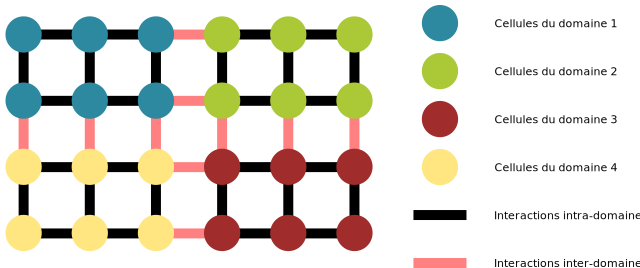
\includegraphics[width=\textwidth]{domain}
  \caption{Décomposition de domaine d'un réservoir à 24 cellules. Il y a deux partitions, chaque partition pouvant être traité en parallèle.}
  \label{fig:domain}
\end{figure}

En utilisant la méthode de Schwarz additive, ce préconditionneur est totalement parallèle et il ignore les interactions inter-domaines.
%
Malheureusement, plus il y a d'interactions ignorées, moins le préconditionneur est efficace.
%
Formulé différemment, le nombre de domaines aura un impact la convergence du GMRES.
%
Cet impact n'est pas facilement prédictible et dépendra du problème étudié.
%
Il est donc quasiment impossible de connaître le nombre de domaine optimal pour avoir un bon rapport parallélisme sur nombre d'itérations du GMRES.
%
C'est pourquoi nous allons essayer de réduire au minimum le nombre de domaines pour toujours obtenir les meilleurs performances.
%
Pour cela, nous allons devoir utiliser une autre forme de parallélisme qui s'appliquera à l'intérieur d'un domaine.
%
Nous allons essayer de paralléliser les différentes étapes du GMRES sans affecter la convergence.

%-------------------------------
\subsection{Cas d'étude}
Pour être en mesure de tester notre méthode de parallélisation en mémoire partagée, nous utilisons un code de solveur linéaire développé à Total SA.
%
Nous allons essayer de paralléliser la partie RAS~\footnote{Restrictive Additive Schwartz} du code.
%
Dans le but d'évaluer le gain de performance, nous avons choisi des systèmes linéaires à résoudre avec le solveur linéaire.
%
Nous allons utiliser le cas test SPE10, ce cas est basé sur les données prises du second modèle du 10ème cas test SPE\cite{SPE10}.
%
C'est un réservoir de 1~122~000 de cellules, organisées dans une grille 3D cartésienne de taille 60 x 220 x 85, il s'agit de schéma de discrétisation en 7 points et c'est un problème de référence dans l'industrie du pétrole.
%
Les autres cas tests seront générés par un programme développé en interne, et il s'agit aussi d'un schéma de discrétisation en 7 points (e.g., volume fini).
%
Il génère des cubes 3D cartésiens de taille arbitraire.
%
Ces cas générés nous permettent de tester énormément de combinaisons de tailles dans le but d'évaluer le passage à l'échelle de nos algorithme.

%+++++++++++++++++++++++++++++++


%+++++++++++++++++++++++++++++++
\section{\'Evolution des architecture}
%-------------------------------
\subsection{Processeurs mono-coeur}
Pour être capable de simuler de grands problèmes physiques, nous avons besoin de beaucoup de puissance de calcul.
%
Cette puissance se mesure en FLOPS\footnote{FLoating-point Operations Per Second}, il s'agit du nombre d'opérations par seconde qu'un ordinateur peut effectuer sur des nombres à virgules flottantes.
%
Même les processeurs mono-coeur peuvent faire des opérations en parallèle.
%
Le parallélisme au niveau instruction en est un bon exemple, les pipelines d'instructions permettent de paralléliser les différentes étapes liées au traitement d'une exécution.
%
Dans l'idéal, le processeur utilisant un pipeline d'instruction pourra exécuter une opération par cycle, donc un processeur à 4~GHz aura une puissance de calcul de 4~GFLOPS si les opérations flottantes sont faites en 1 cycle.


Par la suite, les processeurs ont gagnés des instructions permettant d'effectuer une même opération sur des données différentes, aussi appelées instructions SIMD dans la taxonomie de Flynn.
%
Ces processeurs dits vectoriel peuvent donc avoir une puissance de calcul supérieur, si une instruction est capable d'effectuer 4 opérations à la fois et qu'il tourne à 4~GHz, alors il aura une puissance de calcul de 16~GFLOPS.
%
Il s'agit ici d'une puissance théorique, tous les codes de calculs n'ont pas la possibilité d'exploiter les instructions vectorielles.
%
Ces instructions sont souvent utilisées dans les noyaux de calculs d'algèbre linéaire dense.
%
En simulation de réservoir, nous utilisons ces noyaux de calculs sur les blocs de nos matrices.

%-------------------------------
\subsection{Processeurs multicoeurs}
Pour obtenir encore plus de parallélisme, il est possible de multiplier les unités de calcul au sein d'un processeur.
%
Ces unités de calcul, aussi appelées coeurs de calcul, peuvent être considérées comme des processeurs.
%
Chaque coeur a son propre pipeline d'instructions, ses registres et ses unités arithmétiques.
%
Les coeurs partagent un ou plusieurs niveaux de cache entre eux ainsi que le bus d'accès à la mémoire.
%
Ces caches sont le plus souvent cohérents entre eux, c'est à dire que pour chaque coeur de calcul l'accès à une variable en mémoire retourneras toujours le dernier résultat connu par tous les coeurs de calcul.
%
La cohérence est assurée par un protocole de cohérence de type MOESI\footnote{MOESI est l'acronyme de Modified, Owned, Exclusive, Shared et Invalid qui correspond aux différents états d'une ligne de cache.}.
%
Les caches partagés entre différents coeurs permettront réduire la complexité du mécanisme de cohérence des caches et aussi de bénéficier des données déjà pré-chargée par un autre coeur de calcul.
%
Par contre, la taille du cache est donc partagée entre plusieurs coeurs de calcul et si un coeur demande souvent de nouvelles lignes de cache, le cache deviendra inutilisable et le deuxième coeur aura des problèmes de latence mémoire.
%
Les caches de plus bas niveaux (L1 et parfois L2) sont souvent dédiés à un coeur de calcul, l'espace mémoire n'est donc plus partagée.
%
Mais il peut y avoir des effets négatifs, si deux coeurs de calcul écrivent souvent dans la même ligne de cache, il y a un problème de faux partage et la ligne de cache fait souvent des aller-retour entre les caches dédiés.



La puissance de calcul d'un processeur à 4 coeurs composés d'unités vectorielles et chaque coeur tournant à 4~GHz est de 64~GFLOPS.
%
Encore une fois, cette puissance de calcul est théorique, il faut que le programme puisse utiliser tous les coeurs du processeur ainsi que les instructions vectorielles.
%
Pour pouvoir utiliser tous les coeurs, il faut utiliser du parallélisme multicoeur.

%-------------------------------
\subsection{SMP}
A l'intérieur de chaque noeud d'une grappe de calcul, on peut trouver plusieurs processeurs.
%
Ces processeurs se partagent les ressources disponibles sur la carte mère, cela inclut les entrées/sorties et la mémoire.
%
La façon d'inter-connecter tous les processeurs avec la carte mère peut différer entre différentes architectures.
%
Avec l'architecture SMP, tous les processeurs sont connectés à un bus de données et un arbitre choisit quel processeur peut utiliser le bus à un instant donné (Fig.~\ref{fig:smp}).
%
Cette conception ne passe pas à l'échelle au niveau des performances quand le nombre de processeurs grandit.
%
La bande passante est partagée par tous les processeurs et l'arbitre du bus devient un goulot d'étranglement.
%
Pire, la latence d'un accès mémoire va dépendre de la congestion du bus mémoire.

%   (-_-)   %
\begin{figure}[!ht]
        \centering
        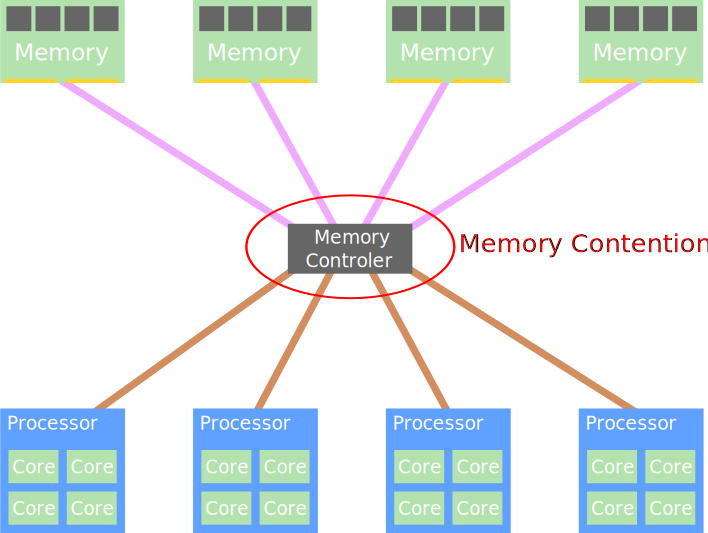
\includegraphics[width=0.8\textwidth]{smp}
        \caption{Vue d'ensemble d'une architecture à accès mémoire uniforme (SMP)}
        \label{fig:smp}
\end{figure}

%-------------------------------
\subsection{NUMA}
Pour dépasser les limites de l'architecture SMP, la mémoire peut être physiquement distribuée entre chaque processeur (Fig.~\ref{fig:numa}).
%
Avec l'architecture NUMA, la latence et la bande passante de chaque accès mémoire dépendent de la distance entre le processeur qui fait la demande et la position physique de la mémoire.
%
Il existe différents moyens d'inter-connecter les processeurs, on peut connecter tous les processeurs un à un pour faire en sorte que la latence soit la plus faible possible, mais tout comme l'architecture SMP cette méthode ne passe pas à l'échelle.
%
Il est aussi possible de limiter le nombre de connexions par processeur tout en optimisant le nombre maximum de sauts, comme fait dans les grappes de calcul.



Chaque saut aura pour effet d'augmenter le temps de latence de l'accès mémoire.
%
La distance entre chaque banc NUMA est fournie par le constructeur de la machine sous la forme d'une matrice de distance.
%
Il existe souvent une correspondance entre la distance fournie par le constructeur et la latence mesurée.
%
Nous pouvons donc utiliser cette matrice pour retrouver la topologie des noeuds NUMA de la machine.
%
La puissance théorique est la même que pour une machine SMP, mais en pratique nous obtenons de meilleures performances grâce à la distribution des bancs mémoires.
%
En contrepartie, pour obtenir ces performances, il est nécessaire d'avoir une bonne gestion de la mémoire.
%
Cette gestion peut-être faite par le noyau du système d'exploitation dans un premier temps puis affinée par le programme lui-même.
%
La plupart des machines NUMA sont ccNUMA\footnote{cache coherent NUMA}, c'est-à-dire que les caches de données sont cohérents entre chaque processeur.
%
Les machines que nous allons utiliser sont toutes ccNUMA, cela signifie qu'une écriture sur un banc NUMA distant coûtera plus cher qu'une lecture.

%   (-_-)   %
\begin{figure}[!h]
  \centering
  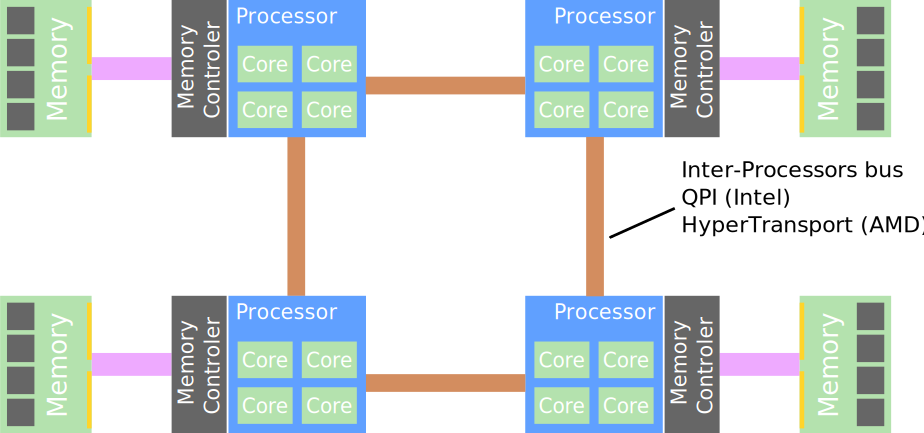
\includegraphics[width=0.8\textwidth]{numa}
  \caption{Vue d'ensemble d'une architecture NUMA.}
  \label{fig:numa}
\end{figure}

%-------------------------------
\subsection{Grappe de serveurs}
Finalement, il est possible de connecter plusieurs ordinateurs entre eux pour obtenir une machine encore plus puissante.
%
Dans une grappe de serveurs, chaque ordinateur est appelé noeud de calcul, il a sa propre mémoire, fait tourner son propre système d'exploitation et peut être considéré comme une machine isolée.
%
Les noeuds sont reliés entre eux par un réseau à faible latence/haut débit, tel que Infiniband ou Myrinet.
%
Le principal avantage de cette solution est le passage à l'échelle.
%
Il est possible de construire des machines de très grandes tailles et très puissantes.

Parmi les 500 machines les plus puissantes du monde au moment de l'écriture de cette thèse, 429 sont des grappes de serveurs.
%
La machine la plus puissante est la {\em TIANHE-2} avec une puissance crête d'environ 55~PFLOPS.
%
Mais l'utilisation de ces machines pose un sérieux problème, elles ne sont pas vraiment faciles à programmer.
%
Il faut prendre en compte que la mémoire n'est pas globale, chaque noeud ne voit que sa mémoire locale.

%-------------------------------
%\subsection{Many-core}
Another solution, used by Intel in the Xeon Phi coprocessor, is to use a ring bus (See Fig~\ref{fig:interconnect}).
%
Memory is distributed over the ring bus just as core units.
%
Why is it better than an SMP ?
%
During my thesis, I had the opportunity of trying a Xeon Phi.


%   (-_-)   %
\begin{figure}[!ht]
  \centering
  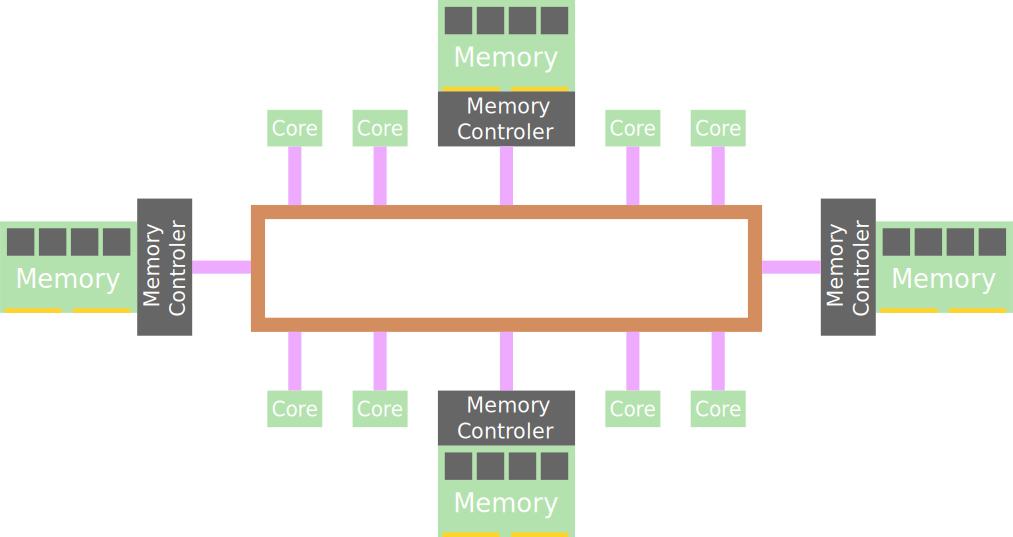
\includegraphics[width=0.8\textwidth]{interconnect}
  \caption{Overview of Xeon Phi Architecture}
  \label{fig:interconnect}
\end{figure}

  \begin{itemize}
    \item Xeon phi
    \item GPU ?
    \item Too many change in program but not always performance (data transfer)
  \end{itemize}

%-------------------------------
\subsection{Nos machines}
Dans le but d'étudier différents problèmes liés à la programmation par tâche, nous avons sélectionné deux machines avec des architectures différentes.


\subsubsection{Rostand}
Rostand est une grappe de serveurs appartenant à la compagnie Total S.A..
%
Elle est composée de 640 noeuds de calcul interconnectés avec un réseau Infiniband.
%
Chaque noeud est lui-même composé de 2 bancs NUMA avec un processeur Intel Xeon X5660 et 24~Go de mémoire par banc NUMA (Fig.~\ref{fig:rostand}).
%
Les processeurs ont 6 coeurs, soit un total de 12 coeurs par noeud de calcul et 7680 coeurs pour l'ensemble de la grappe.


%   (-_-)   %
\begin{figure}[!h]
        \centering
        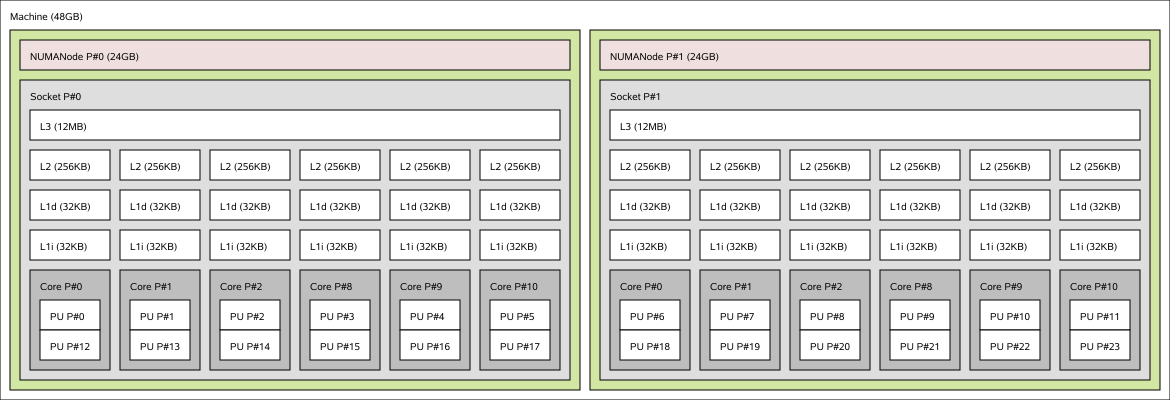
\includegraphics[width=\textwidth]{rostand_lstopo}
        \caption{Topologie d'un noeud de calcul de Rostand. Le schéma a été obtenu avec le logiciel hwloc.}
        \label{fig:rostand}
\end{figure}

Avec cette machine, nous allons pouvoir tester deux paradigmes de programmation parallèle.
%
Dans un premier temps nous utiliserons du parallélisme intra-noeud puis nous verrons le parallélisme inter-noeud.


La matrice des distances (Fig.~\ref{fig:rostand_distance}) nous indique la distance entre deux bancs NUMA donnée par le constructeur de la machine.
%
Cette distance est adimensionnée, la distance entre un banc NUMA et lui-même est égale à 10, les autres distances sont mises à l'échelle par rapport à 10 comme spécifié dans la norme ACPI.
%
Ces distances sont obtenues avec la commande {\em ``numactl --hardware''} sous Linux.
%
\'Etant donné que cette valeur ne peut servir qu'à connaître la topologie des bancs NUMA, nous avons décidé de mesurer la latence mémoire entre chaque banc.
%
Pour cela, nous avons utilisé l'outil {\em lmbench} couplé à {\em numactl} pour définir les bancs NUMA à utiliser.
%
Nous savons donc qu'un accès à un banc NUMA distant a un temps de latence 57~\% plus grand qu'un accès au banc NUMA local.


%   (-_-)   %
\begin{figure}[!h]
        \centering
        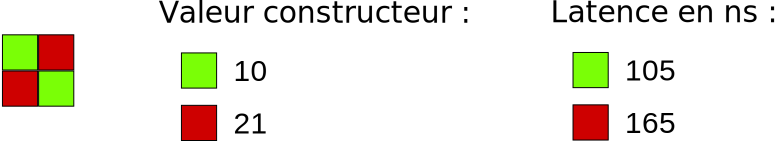
\includegraphics[width=0.5\textwidth]{rostand_distance}
        \caption{Matrice des distances entre chaque banc NUMA de Rostand.}
        \label{fig:rostand_distance}
\end{figure}

\subsubsection{Manumanu}
Manumanu est une machine Altix UV100, cet ordinateur est composé de 20 bancs NUMA.
%
Chaque banc NUMA est composé d'un processeur Intel Xeon E7-8837 ainsi que de 32~Go de mémoire.
%
Les processeurs ont chacun 8 coeurs de calcul, pour un total de 160 coeurs et 640~Go de mémoire partagée.
%
Cette machine est vraiment intéressante pour évaluer les effets NUMA.

%   (-_-)   %
\begin{figure}[!h]
     \begin{center}
        \subfigure[Matrice des distances entre chaque banc NUMA.]{%
          \label{fig:manumanu_distances}
          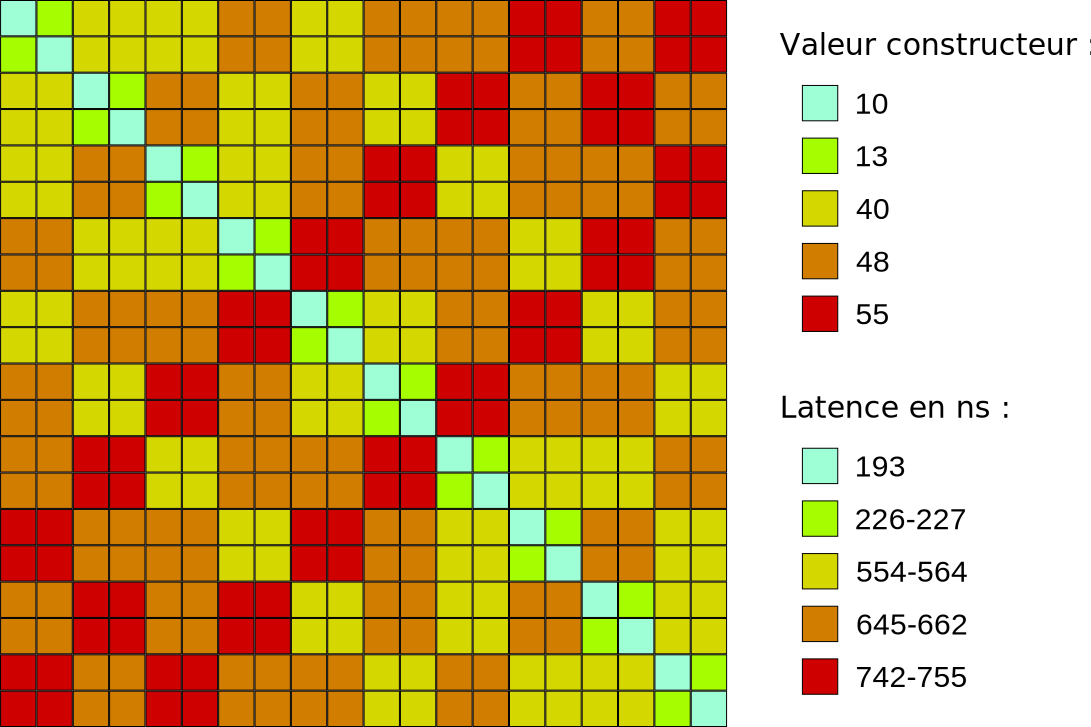
\includegraphics[width=0.59\textwidth]{manumanu_distance}
        }%
        \subfigure[Topologie déduite de la matrice des distances. Chaque noeud représente un groupe de deux bancs NUMA.]{%
          \label{fig:manumanu_topo}
          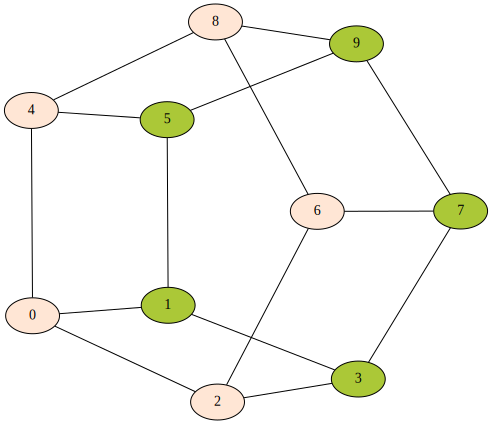
\includegraphics[width=0.39\textwidth]{manumanu_topologie}
        }%
    \end{center}
    \caption{Architecture de Manumanu.}
    \label{fig:manumanu}
\end{figure}

\`{A} partir de la matrice des distances (Fig.~\ref{fig:manumanu_distances}), nous pouvons déduire la topologie de la machine.
%
Les bancs NUMA sont regroupés deux par deux et chaque groupe est connecté à trois autres groupes.
%
Ce regroupement permet de limiter la distance maximal entre deux banc NUMA, il y aura au maximum 3 sauts.
%
Les temps de latence entre deux bancs NUMA d'un même groupe n'est supérieur que de 17\% par rapport à un accès local.
%
Par contre, les temps de latence entre deux groupes sont entre 3 et 4 fois plus long qu'un temps de latence local.

%+++++++++++++++++++++++++++++++


%+++++++++++++++++++++++++++++++
\section{Parallélisme multi-coeur}
%-------------------------------
Lorsque l'on souhaite paralléliser un code de calcul, on doit choisir parmi plusieurs paradigme de parallélisation.
%
Le choix de ce paradigme est une étape importante, elle déterminera les algorithmes à utiliser et donc aussi les performances du programme.
%
En effet, un même problème ne se résoudra pas de la même façon en fonction du paradigme choisi.
%
Mais le choix du paradigme est aussi déterminé par l'architecture de la machine cible.
%
Dans le cas d'une grappe de serveurs, les noeuds de calculs ne peuvent communiquer que par un réseau.
%
On préféra donc utiliser un paradigme par passage de messages ce qui nous obligera à utiliser des algorithmes distribués.
%
Alors que dans le cas d'une machine à mémoire partagée nous aurons recours à l'utilisation de processus légers, aussi appelé {\em thread}.
%
Plusieurs paradigmes peuvent être utilisés ensemble, nous pouvons ainsi tirer parti des avantages de chacun tout en limitant leurs inconvénients.
%
Nous allons maintenant détailler les différents paradigmes de parallélisation que nous avons utilisé.

%-------------------------------
\subsection{Passage de messages}
Certaines machines ne fonctionnent pas avec une mémoire globale, chaque noeud de calcul a une mémoire locale et il ne peut pas accéder directement à la mémoire des autres noeuds distants, ces machines sont dites à mémoire distribuée.
%
Avec le paradigme de passage de messages, chaque processus a son propre espace mémoire virtuel et communique avec les autres processus par le biais d'envoi/réception de messages.
%
Ces communications se font à l'aide d'une interface de programmation qui fournit des fonctions permettant l'échange de messages point-à-point.
%
L'interface la plus connue et la plus utilisée actuellement est MPI\footnote{Message Passing Interface}.
%
Elle permet de faire communiquer deux processus ensemble sans se soucier du réseau utilisé ou même de la différence d'endianness entre deux architectures différentes.


L'un des avantages majeur de ce paradigme est qu'il permet d'utiliser un ensemble très varié de machine.
%
Il fonctionne aussi en mémoire partagée qu'en mémoire distribuée.
%
Par contre, certains algorithmes ne peuvent pas être écrits efficacement avec ce paradigme.
%
Dans notre cas, la factorisation d'une matrice creuse se parallélise très mal.
%
Nous sommes obligés de modifier les méthodes de factorisation pour être capable d'obtenir de la performance.

%-------------------------------
\subsection{Parallélisme de boucle}
Le parallélisme de boucle est un paradigme qui peut être utilisé sur des machines à mémoire partagée.
%
Il s'agit de traiter en parallèle toutes les itérations d'une boucle en les distribuant équitablement sur tous les coeurs de calcul disponibles.
%
Il faut bien sûr que ces itérations soit indépendantes, c'est à dire qu'avec un nombre infini de coeur de calcul, on pourrait traiter une itération par coeur simultanément.
%
Ce paradigme fonctionne de la manière suivante : un thread est crée par coeur de calcul et chaque thread doit s'occuper de traiter une partie des itérations de la boucle.
%


L'interface de programmation qui a le plus démocratisé ce paradigme est OpenMP.
%
Cette interface utilise les directives de compilation en C qui ont l'avantage d'être simple à utiliser et elles peuvent se désactiver facilement pour retrouver un code séquentiel.
%
En ajoutant la fameuse directive ``\#pragma omp parallel for'' juste au-dessus d'une boucle for, on obtient facilement un programme multi-threadé, la description du parallélisme est très simple.
%
Les performances obtenues avec ce paradigme sont souvent suffisantes pour un grand nombre de logiciel et le ratio entre le temps de développement et le gain en temps d'exécution est imbattable.
%
Malheureusement, il peut arriver qu'il y ai des dépendances de données entre deux itérations, dans ce cas, ce paradigme de parallélisation donnera un résultat faux et il faudra utiliser un autre paradigme.

%-------------------------------
\subsection{Parallélisme à base de tâches}
Pour représenter le parallélisme à base de tâches, nous utilisons des graphes orientés acycliques, ou DAG\footnote{Directed Acyclic Graph}.
%
Dans ce modèle, les n{\oe}uds du graphe représentent une action à effectuer et les arêtes représentent l'ordre séquentiel entre deux actions.
%
Ainsi, nous pouvons représenter le parallélisme sous une forme abstraite indépendamment des ressources matérielles disponibles.
%
Il existe de nombreux travaux appliquant ce principe et permettant ainsi de paralléliser efficacement des codes de calcul~\cite{BBAC2014,LSAT2013,LY2012,ABGL2013}.
%
La démocratisation des processeurs multi-coeurs a engendrée l'apparition de cadriciels à base de tâches~\cite{taskscomparison} comme illustré par des outils tel que Intel TBB~\cite{Intel_TBB} et que le support des tâches dans OpenMP~3.0~\cite{openmptasks} pour du parallélisme multi-coeur, ou StarSs/OmpSs~\cite{OMPSs} ainsi que StarPU~\cite{starpu} et X-Kaapi~\cite{xkaapi} pour le support de plateformes hétérogènes.
%
Dans ces modèles, la granularité correspond au nombre d'instructions processeur contenues dans la tâche.
%
Cette granularité dépend de l'algorithme à paralléliser ainsi que de l'ordonnanceur de tâches.

%+++++++++++++++++++++++++++++++


%+++++++++++++++++++++++++++++++
\section{Runtime}
%-------------------------------
\subsection{Vue d'ensemble}
Un moteur d'exécution, ou {\em runtime}, est un morceau de logiciel utilisé par d'autres logiciels pour abstraire des parties du système.
%
L'idée principale est {\em compiler une fois, exécuter partout}.
%
Ils sont présent un peu partout et peuvent avoir différentes fonctions.
%
Certains langages dits de haut niveau utilisent un runtime, par exemple Java a un runtime pour gérer son ramasse-miettes.
%
Toutes les implémentations de MPI ont un runtime.
%
Les cadriciels de programmation à base de tâches tendent à utiliser un runtime.
%
Les parties suivantes se concentreront sur le support des runtimes pour la programmation à base de tâches.


Les runtimes utilisés pour la programmation à base de tâches doivent en premier lieu être capable d'ordonnancer le traitement des tâches tout en respectant l'ordre des dépendances entre les tâches (Fig.~\ref{fig:runtime}).
%
Ces runtime doivent aussi fournir un équilibrage de charge entre toutes les ressources matérielles disponibles (potentiellement hétérogènes) dans le but de minimiser le temps de calcul.
%
Certains runtimes s'occupent de transférer des données entre deux ressources potentiellement hétérogènes, comme par exemple entre la mémoire principale et la mémoire d'une carte graphique ou plus simplement entre deux processus.
%
Ces transferts peuvent être implicites, le runtime a connaissance des données qui sont manipulées, ou ils peuvent être explicites avec l'utilisation d'une tâche spéciale qui s'occupera de faire les échanges de données.

%   (-_-)   %
\begin{figure}
  \centering
  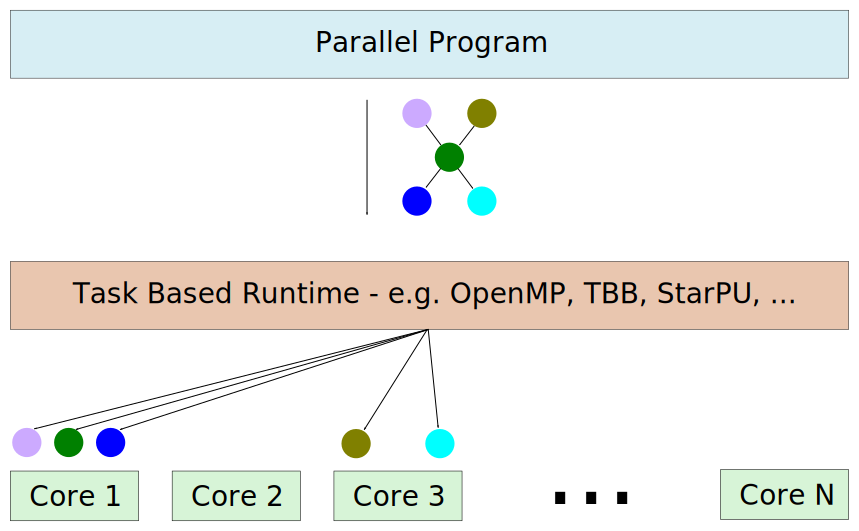
\includegraphics[width=0.8\textwidth]{runtime}
  \caption{Le programme parallèle fournit un graphe de tâches à l'ordonnanceur de tâches. Les tâches sont ensuite distribuées sur les coeurs de calcul disponibles.}
  \label{fig:runtime}
\end{figure}


Pour améliorer l'équilibrage de charge, les runtimes ont des politiques d'ordonnancement, la plupart de ces politiques sont dynamiques et peuvent s'adapter à la charge courante de la machine.
%
D'autres politiques d'ordonnancement, dîtes statiques, permettent de réduire le coût d'ordonnancement.
%
L'ordonnanceur parfait n'existe pas et n'existera sûrement jamais.
%
En effet, trouver le meilleur ordonnancement d'un ensemble de tâches avec un nombre limité de ressources de calcul est un problème NP-complet\footnote{Un problème est NP-complet si le temps nécessaire à la résolution du problèmes est polynomial comparé à la taille des données en entrées et que ce problème soit aussi difficile que tous les autres problèmes NP-complets.}.
%
Il existe des heuristiques d'ordonnancement qui donnent de bons résultats dans la majorité des cas, nous pouvons citer l'algorithme HEFT\cite{heft}.
%
Si le modèle de programmation le permet, des informations additionnelles peuvent être attribuées aux tâches, comme par exemple une estimation du temps de calcul, ces informations sont ensuite utilisées par l'ordonnanceur pour améliorer le placement des tâches.


L'apparition des premières machines parallèles à mémoire partagée a conduit à la recherche de nouvelles méthodes pour les programmer.
%
Il faut donc distribuer une charge de travail sur plusieurs unités de calcul.
%
Malheureusement, il arrive que cette charge de travail de soit pas connu l'avance.
%
Une idée est alors apparu pour rendre cette distribution plus flexible : le vol de travail (ou {\em work-stealing} en anglais).
%
Dès qu'une ressource de calcul n'as plus de travail, elle essaye de voler du travail à une autre ressource.
%
Le langage Cilk~\cite{Cilk}, apparu en 1994 et toujours développé sous le nom Cilk++~\cite{Cilk++}, permet de faire du vol de travail.
%
Les tâches sont décrites par le programmeur avec des mots clés additionnels au langage C, par exemple le mot-clé {\em spawn} placé avant l'appel d'une fonction permet à Cilk de comprendre qu'il doit créer une nouvelle tâche et qu'il doit l'ordonnancer.
%
Ces tâches sont empilées sur une pile spécifique à chaque thread.
%
Le vol de tâche se fait par le biais de cette pile de tâches (Fig.~\ref{fig:task_steal}).

%   (-_-)   %
\begin{figure}[t!]
  \centering
  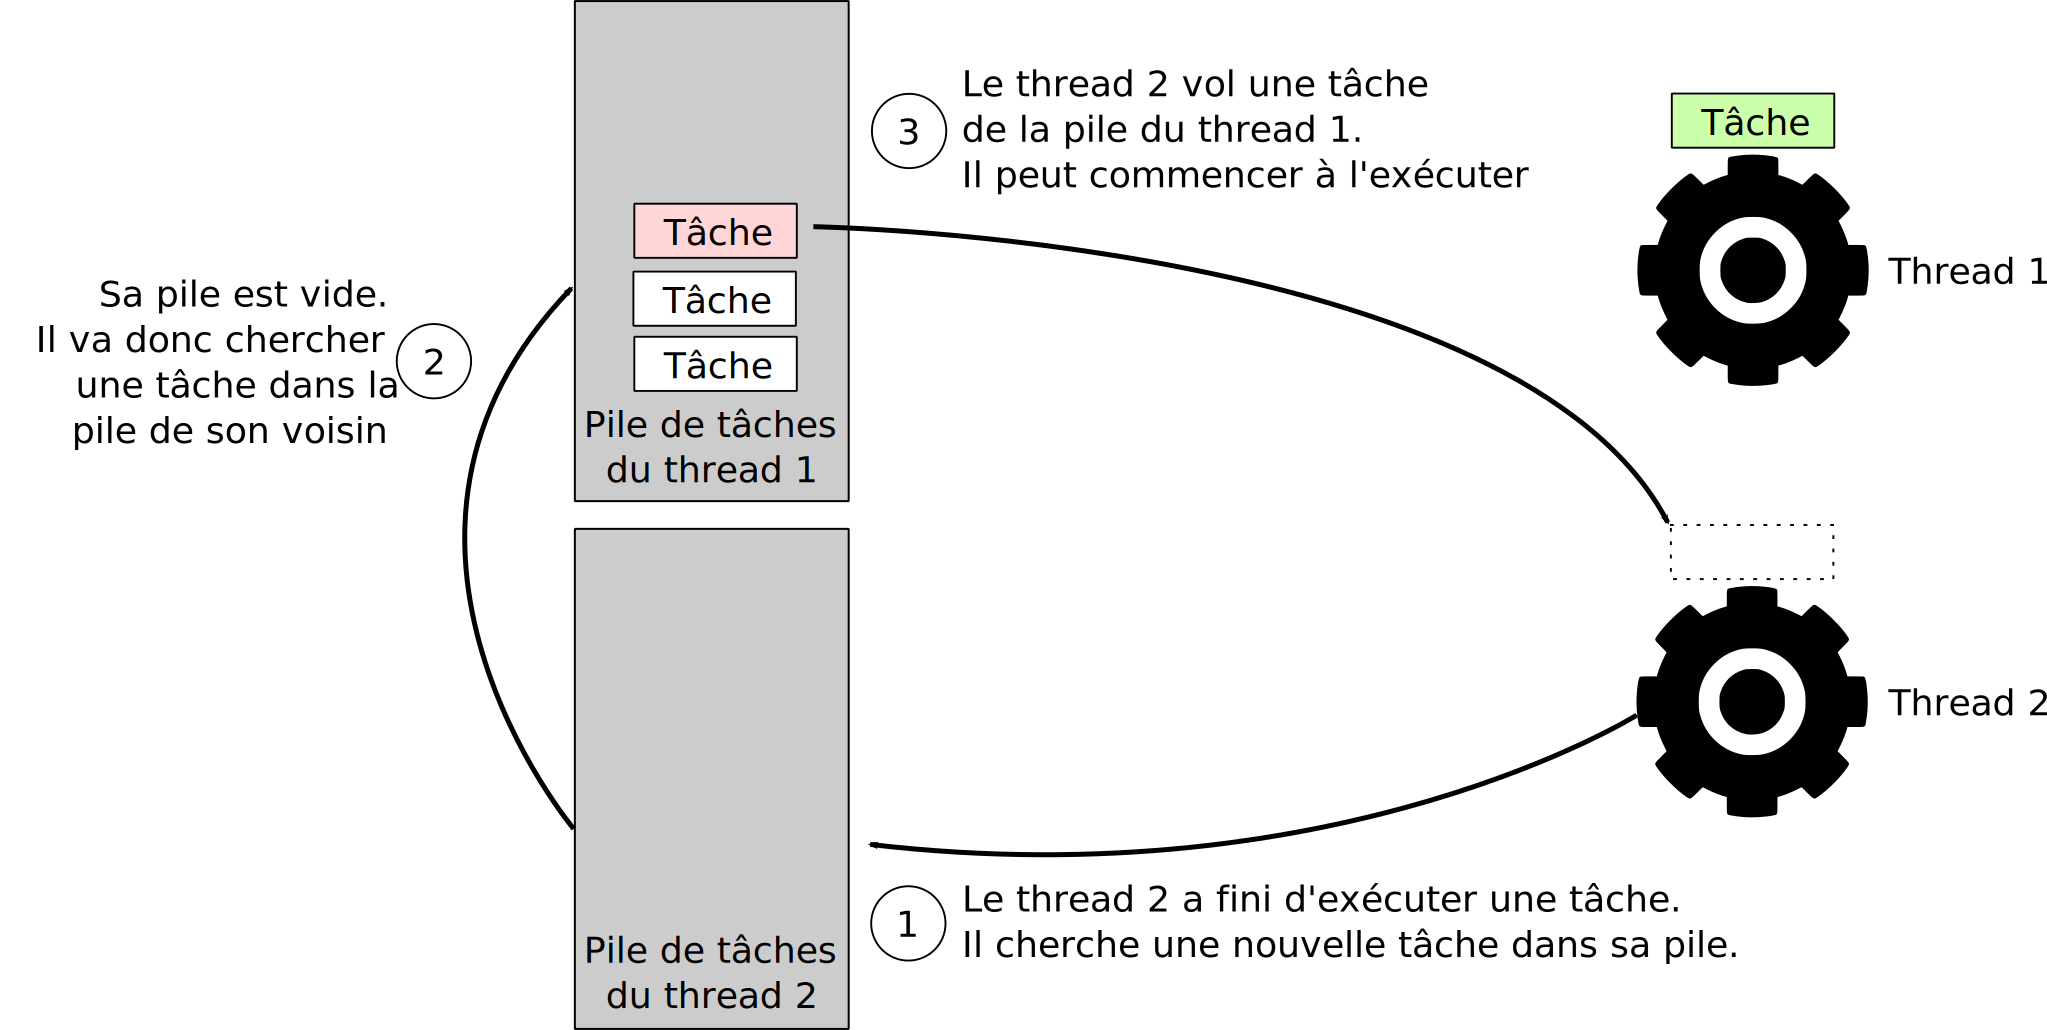
\includegraphics[width=\textwidth]{task_steal}
  \caption{Vol de tâche du thread 2 dans la pile du thread 1.}
  \label{fig:task_steal}
\end{figure}




Peu de temps après, en 1997, une interface de programmation parallèle voit le jour, il s'agit d'OpenMP~\cite{OpenMP}.
%
Les premières versions d'OpenMP se concentrent sur le parallélisme de boucle.
%
En ajoutant des annotations autour d'une boucle for, les itérations de la boucle seront distribuées sur les coeurs de calcul.
%
Il existe aussi des annotations permettant d'effectuer des réductions à la fin de la boucle.
%
Ce n'est qu'en 2008 que le support des tâches est ajouté à OpenMP dans sa version 3.0~\cite{openmptasks}.
%
Le programmeur peut créer des tâches parallèles mais il n'y a aucun moyen de spécifier les dépendances entre les tâches.
%
Les graphes de tâches ne peuvent donc pas être directement utilisés dans OpenMP.
%
OpenMP est donc un runtime très complet pour faire du parallélisme de boucle mais son modèle de tâches se rapproche du modèle de Cilk.


Intel TBB~\cite{Intel_TBB}, dont le développement a démarré en 2006, permet aussi de faire du parallélisme à base de tâches.
%
La gestion des dépendances entre les tâches est à la charge du programmeur mais TBB fournit les méthodes nécessaires telles que l'incrémentation et la décrémentation atomique du compteur de référence d'une tâche.
%
Le modèle d'abstraction du matérielle dans TBB ne permet pas de connaître le nombre de threads utilisés.
%
Ce choix est fait parce que pour Intel le programmeur n'a pas a se soucier des problèmes d'ordonnancement.




Plus récemment, à la fin des années 2000, la révolution du GPGPU donne lieu à l'apparition de nouveaux runtimes.
%
Les premières méthodes permettant d'utiliser un GPU pour du calcul étaient rudimentaires.
%
Il s'agissait de détourner l'utilisation des shaders programmables des interfaces de programmation graphiques comme par exemple OpenGL.
%
Puis des langages spécifiques ont vus le jour, parmi ceux ci, les plus populaires sont CUDA et OpenCL.
%
CUDA est développé par NVidia et ne permet de programmer que des GPU NVidia.
%
OpenCL est une spécification du Khronos Group et a pour but de fournir une interface de programmation standard pour programmer toutes sortes d'accélérateurs.
%
Ces accélérateurs peuvent être des GPUs mais de manière générale il s'agit de co-processeurs déportés.



StarPU~\cite{starpu}, développé à Inria permet de d'écrire plusieurs versions d'une routine à la fois pour le CPU et le GPU.
%
Ces morceaux de codes spécifiques à une architecture sont appelés {\em codelets}.
%
Puis les stratégies d'ordonnancement intégrées à StarPU choisiront la codelet qui permettra d'obtenir le meilleur temps de calcul.
%
Ce choix prend aussi en compte le temps de transfert mémoire entre la mémoire centrale et la mémoire du GPU.
%
Pour avoir une gestion efficace de ces transferts mémoires, StarPU implémente un gestionnaire mémoire.
%
Ce gestionnaire est capable d'effectuer des transferts entre toutes les zones mémoires de la machine (mémoire centrale, mémoire GPU, disques, ...) et de maintenir la cohérence des données.
%
Par exemple, si une donnée A est en mémoire centrale et qu'une codelet doit l'utiliser sur le GPU, il y aura d'abord une copie A vers la mémoire du GPU.
%
Ensuite tant que cette donnée n'est accédée qu'en lecture, il y aura deux copies valides, une en mémoire centrale et une en mémoire GPU.
%
Dès qu'une codelet accède à la donnée en écriture, toutes les autres copies sont invalidées et un transfert mémoire sera nécessaire pour les mettre à jour.
%
StarPU intègre aussi plusieurs politiques d'ordonnancement permettant d'adapter à plusieurs code de calcul.
%
L'équipe de développement met aussi en avant la possibilité d'écrire son propre ordonnanceur et de l'intégrer à StarPU.


X-KAAPI~\cite{xkaapi} est aussi développé à Inria et permet de programmer des applications qui auront du code qui sera exécuté à la fois sur CPU et sur GPU.
%
Il se différencie de StarPU par son système de vol de tâches dynamique.
%
X-KAAPI va partitionné le graphe de tâches et distribuer les partitions aux threads.
%
Chaque thread a ainsi une première approximation de l'ordonnancement du graphe.
%
Le surcoût de gestion des dépendances est ainsi limité aux frontières entre les partitions.
%
Lors de l'exécution du code, si un thread se retrouve à court de tâches, il va essayer d'en voler à un autre thread que l'on appellera {\em victime}.
%
Mais il ne va pas la voler complètement, il la laisse dans la pile de la victime en ajoutant comme information que la tâche a été volée.
%
Ainsi lorsque la victime découvrira qu'une tâche a été volée, elle devra vérifier les dépendances de cette tâche.
%
Ce système permet de réduire le surcoût d'ordonnancement, avec un bon partitionnement, le vol de tâche est plus rare et beaucoup de temps a été économisé sur la gestion des dépendances.



OmpSs~\cite{OMPSs} est un runtime qui permet, tout comme StarPU et X-KAAPI, d'écrire du code à la fois pour le CPU et pour le GPU puis de laisser le runtime choisir parmi toutes les versions d'une fonction.
%
La différence entre ces deux runtimes provient surtout de la description du parallélisme.
%
OmpSs propose un approche à base d'annotation de code en étendant la spécification OpenMP version 3.
%
Cette extension permet au mot clé {\em task} d'être accompagné d'informations complémentaires sur l'utilisation des paramètres en entrée.
%
OmpSs pourra ensuite déduire les dépendances entre les tâches depuis les informations sur les paramètres en entrée.
%
Il n'y a pas non plus d'écriture automatisée de code, le programmeur doit toujours écrire le code spécifique à chaque architecture précédé d'informations concernant la fonction implémentée ainsi que l'architecture cible.


HMPP~\cite{hmpp} est un runtime, développé par CAPS, adressant le problème de la programmation hybride CPU/GPU.
%
Il s'utilise avec des annotations de code de la même manière qu'OpenMP et qu'OmpSs.
%
Puis le code annoté est ensuite transformé par un compilateur source-to-source vers un autre langage spécifique à l'architecture cible, comme le CUDA par exemple.
%
Les transferts mémoires entre la mémoire centrale et la mémoire du GPU peuvent être fait de deux façons :
\begin{itemize}
  \item implicitement au moment de l'appel de la codelet mais cette méthode ne permet de recouvrir la communication par du calcul;
  \item explicitement avec l'ajout d'annotation, il est donc à la charge du programmeur de choisir le bon moment pour transférer les données.
\end{itemize}
%



OpenACC~\cite{OpenACC} est un standard de programmation développé par un consortium de société dans le but de simplifier la programmation parallèle hybride CPU/GPU.
%
Les spécificités de ce standard ressemble en de nombreux points à HMPP (annotations, gestion mémoire, ...).
%
Son principal avantage est qu'il est soutenu par plusieurs sociétés là où HMPP n'est plus supporté.
%
OpenMP ajoute dans version 4 le support de la programmation hybride, son fonctionnement est identique à OpenACC, seuls les mot-clés changent.


PaRSEC~\cite{PaRSEC} est un runtime développé à l'ICL permettant de travailler directement en mémoire distribuée.
%
Le parallélisme dans PaRSEC doit être décrit dans un langage spécifique, le JDF.
%
L'ensemble des tâches du programme est décrit dans ce langage et ce n'est que la distribution des données en mémoire distribuée qui détermineras le processus qui exécuteras la tâche.
%
PaRSEC s'occupe automatiquement des communications entre processus permettant de maintenir une cohérence entre les données.
%
L'inconvenient majeur de ce runtime est son manque de flexibilité.
%
Le format JDF ne permet de créer dynamiquement de nouvelle tâche.

%+++++++++++++++++++++++++++++++




%=========================================================
\chapter{Un problème de granularité}
\minitoc
\vspace{1cm}
%=========================================================
%+++++++++++++++++++++++++++++++
\section{Parallélisation de l'algorithme GMRES préconditionné}
%-------------------------------
\subsection{Partie GMRES}
L'algorithme GMRES est utilisé pour résoudre de grands systèmes linéaires creux.
%
La plupart des opérations sont des opérations de type BLAS1 (axpy, dot product...) et sont facilement parallélisables.
%
L'opération la plus coûteuse de l'algorithme du GMRES est le produit matrice vecteur, ou {\em SpMV}\footnote{Sparse Matrix Vector multiply}.
%
Cette opération peut être parallélisée avec du parallélisme de boucle, les lignes de la matrice peuvent être traitées indépendamment les unes des autres.


Donc en général, l'algorithme GMRES se parallélise très bien.
%
Mais nous ne pouvons pas l'utilise tel quel, nos matrices ne sont pas assez bien conditionnée.
%
Il est nécessaire de préconditionner nos matrices pour obtenir de bonnes performances.
%
Par contre, la partie préconditionneur n'est pas toujours facilement parallélisable.
%
Par exemple, le préconditionneur ILU(k), que nous allons utiliser, est un algorithme séquentiel.
%
Ce chapitre sera consacré à rendre cet algorithme plus parallèle.



%% \begin{algorithm}
%%   \fontsize{8pt}{9pt}\selectfont
%%     \begin{algorithmic}[1]
%%       \STATE Compute $r_0 := b - Ax_0$, $\beta := ||r_0||_2$, and $v_1 := r_0/\beta$
%%       \STATE Define the $(m + 1) x m$ matrix $\overset{-}{H}_m = \{h_{ij}\}_{1 \leq i \leq m+1, 1 \leq j \leq m}$. Set $\overset{-}{H}_m = 0$
%%       \FOR{$j=1$ to $m$}
%%         \STATE \tikz[baseline]{\node[fill=yellow!20,anchor=base]{Compute $temp := Triangular\_Solve(M, v_j)$};} \hspace{0.3in} (MPI\_Send(Border\_Cells))
%%         \STATE \tikz[baseline]{\node[fill=red!20,anchor=base]{Compute $w_j := A * temp$};} \hspace{1.2in} (MPI\_Recv(Ghost\_Cells))
%%         \FOR{\tikz[baseline]{\node[fill=blue!20,anchor=base]{$i=1$ to $j$};}}
%%           \STATE \tikz[baseline]{\node[fill=blue!20,anchor=base]{$h_{ij} := (w_j, v_i)$};}
%%           \STATE \tikz[baseline]{\node[fill=blue!20,anchor=base]{$w_j := w_j - h_{ij}v_i$};}
%%         \ENDFOR
%%         \STATE $h_{j+1,j} := ||w_j||_2$.
%%         \IF{$h_{j+1,j} = 0$}
%%           \STATE $m := j$
%%           \STATE \textbf{break}
%%         \ENDIF
%%         \STATE $v_{j+1} := w_j/h_{j+1,j}$
%%       \ENDFOR
%%       \STATE Compute $y_m$ the minimizer of $||\beta{}e_1 - \overset{-}{H}_my||_2$ and $x_m := x_0 + V_my_m$
%%     \end{algorithmic}
%%     \caption{GMRES with Householder orthogonalization from Yousef Saad}
%%   \end{algorithm}

%-------------------------------
\subsection{Partie préconditionneur}
La factorisation LU en algèbre linéaire dense est une méthode pour factoriser une matrice $A$ en deux matrices $L$ et $U$.
%
$L$ est une matrice triangulaire inférieure, toutes les valeurs au-dessus de la diagonale sont nulles.
%
Symétriquement, $U$ est une matrice triangulaire supérieure, toutes les valeurs de $U$ en-dessous de la diagonale sont nulles.
%
Le principal intérêt de cette factorisation est de trouver $x$ dans les équations du type $Ax=y$.
%
Cette équation est transformée en deux équations $L.x_{tmp}=y$ et $U.x=x_{tmp}$.
%
La méthode utilisée pour résoudre les systèmes composés de matrices triangulaires est triviale.
%
Il suffit de résoudre chaque équation ligne par ligne en commençant par la ligne qui n'a qu'une seule valeur non nulle.
%
Ensuite il faut résoudre la ligne avec deux valeurs non nulles dont une des inconnues provient de la solution précédente, et ainsi de suite jusqu'à la dernière ligne.
%
Il existe du parallélisme à exploiter dans cet algorithme, à chaque fois qu'une inconnue est trouvée, on peut la retirer de chacune des lignes restantes à traiter~\cite{plasma_lu}.



En algèbre linéaire creuse, la factorisation LU d'une matrice $A$ creuse donnera deux matrices triangulaires denses $L$ et $U$.
%
Or, dans le cas d'une matrice d'ordre élevé ($>$ 100 000), ces deux matrices ne peuvent pas tenir en mémoire.
%
C'est pourquoi en algèbre linéaire creuse, on utilise une version altérée de cette factorisation que l'on appelle factorisation incomplète, ou {\em ILU}\footnote{Incomplete LU}, dont le but est de limiter le remplissage de la matrice.
%
L'algorithme ILU est similaire à l'algorithme LU mais le remplissage est limité par des conditions définies par l'algorithme.
%
Ces conditions peuvent être de deux formes : soit en limitant le remplissage avec une valeur seuil (ILUT), soit en limitant le niveau d'interaction entre les lignes de la matrices (ILU(k)).
%
Dans le cas ILU(k), le paramètre k sert à limiter le niveau d'interaction entre les lignes.
%
Avec $k=0$, le motif des matrices $L$ et $U$ reste similaire au motif de la matrice $A$.
%
Le parallélisme exploitable dans l'algorithme ILU est différent de celui exploitable dans l'algorithme LU, il offre la possibilité de factoriser certaines lignes en parallèle et ce parallélisme se représente naturellement sous la forme d'un graphe de tâches (Fig.~\ref{fig:example_3_dag}).
%
Chaque tâche représente la factorisation d'une ligne de la matrice et les dépendances entre les tâches sont données par le motif de la matrice.
%
En effet, pour factoriser la ligne $i$, nous devons factoriser toutes les lignes $j$ inférieures à $i$ tel que l'entrée $(i,j)$ de la matrice soit non nulle (Fig.~\ref{fig:example_2_matrix}).
%
Donc, à partir du motif des valeurs non-nulles de la matrice, nous pouvons facilement construire le graphe de tâche:
%
la tâche $i$ corresponds à la ligne $i$ de la matrice, la liste des tâches prédécesseurs de la tâche $i$ est donnée par l'index de colonne des valeurs non-nulles avant la diagonale dans la ligne $i$ et la liste des tâches successeurs de la tâche $i$ est donnée par l'index de ligne des valeurs non-nulles au-dessous de la diagonale de la colonne $i$ (Algo~\ref{algo:ilu0}).

\begin{figure}[!ht]
     \begin{center}
        \subfigure[Un réservoir à 4 cellules]{%
          \label{fig:example_1_res}
          
\includegraphics[width=0.32\textwidth]{example_1_res}
        }%
        \subfigure[Une matrice avec 4 cellules]{%
          \label{fig:example_2_matrix}
          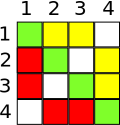
\includegraphics[width=0.32\textwidth]{example_2_matrix}
        }%
        \subfigure[Un DAG à 4 cellules]{%
          \label{fig:example_3_dag}
          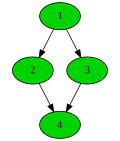
\includegraphics[width=0.32\textwidth]{example_3_dag}
        }%
    \end{center}
    \caption{Trois représentations d'un réservoir. Les éléments en rouge dans la matrice déterminent les dépendances dans le graphe de tâches.}
    \label{fig:exemple_3_dag}
\end{figure}

\begin{algorithm}
  \KwData{$M$ : matrice de dimension $n$}
  \For{$i = 2$ {\bf à} $n$} {
    \For{$k = 1$ {\bf à} $i - 1$ {\bf et} $M_{ik} != 0$} {
      $M_{ik} = M_{ik} / M_{kk}$ \\
      \For{$j = k + 1$ {\bf à} $n$ {\bf et} $M_{ij} != 0$} {
        $M_{ij} = M_{ij} - M_{ik}M_{kj}$ \\
      }
    }
  }
  \caption{Factorisation ILU(0) sur place.}
  \label{algo:ilu0}
\end{algorithm}


En résumé, le parallélisme de l'algorithme ILU peut se représenter sous la forme d'un graphe de tâches.
%
Chaque tâche représentant la factorisation d'une ligne... ce qui est bien petit.
%
En fait, la plupart des runtimes mettront plus de temps à ordonnancer la tâche que la tâche mettra à factoriser une ligne.


Les problèmes rencontrés pour paralléliser la factorisation incomplète d'une matrice creuse, ainsi que les résolutions triangulaires associées, sont des problèmes qui représentent bien la difficulté que l'on peut rencontrer avec une parallélisation à grain fin.
%
La description à grain fin de ces algorithmes est naturelle, mais en pratique, une simple parallélisation utilisant Intel TBB ou OpenMP ne donnera pas de bonnes performances à cause du faible coût de calcul d'une tâche.
%
On appelle cela le problème de granularité.
%
Pour résoudre ce problème, les tâches doivent devenir plus grosses, nous devons factoriser plusieurs lignes à l'intérieur d'une tâche.
%
Mais le choix de ces lignes n'est pas trivial, il faut limiter l'impact sur le parallélisme et ne pas changer le résultat final.
%
Une méthode générique a été développée durant la thèse et sera expliquée plus loin dans ce document.


Il existe des travaux de recherche dont le but est aussi d'exploiter le parallélisme de l'algorithme ILU.
%
En changeant la numérotation des cellules, on peut modifier la structure de la matrice ce qui aura pour effet de changer la factorisation.
%
Une renumérotation rouge-noire permet de factoriser parallèlement la moitié des lignes de la matrice dans un premier temps, puis la seconde moitié des lignes dans un second temps.
%
Cette technique offre énormément de parallélisme mais aura un impact négatif sur la convergence\cite{red_black_ilu}.
%
Plus récemment, une autre méthode a été développée permettant de factoriser tous les éléments de la matrice en parallèle tout en gardant une numérotation naturelle.
%
L'opération de factorisation parallèle est appelé {\em sweep} et doit être effectuée plusieurs fois\cite{chow2014fine}.
%
En moyenne 3 sweeps suffisent à obtenir un résultat proche de la factorisation incomplète.
%
La convergence n'est donc que faiblement dégradée, mais il faut prendre en compte que 3 sweeps ont été nécessaires et il a donc fallu faire 3 fois plus d'opérations qu'une factorisation ILU classique.

%   (-_-)   %
\begin{figure}[!ht]
     \begin{center}
        \subfigure[Exemple de graphe de tâche obtenu avec une numérotation naturelle.]{%
          \label{fig:DAG_natural}
          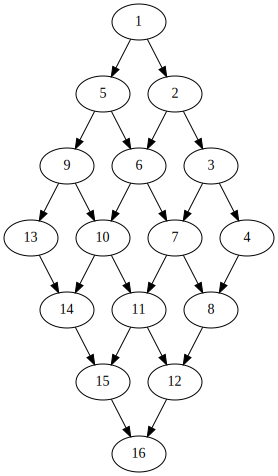
\includegraphics[width=0.33\textwidth]{DAG_natural}
        }%
        \subfigure[Exemple de graphe de tâche obtenu avec une numérotation rouge-noire.]{%
          \label{fig:DAG_redblack}
          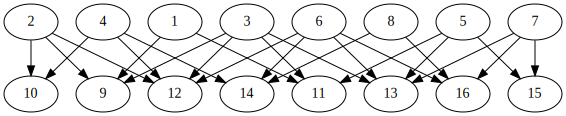
\includegraphics[width=0.66\textwidth]{DAG_redblack}
        }%
    \end{center}
    \caption{Différence de parallélisme en fonction de la numérotation choisie.}
    \label{fig:DAG_ordering}
\end{figure}

%-------------------------------
%+++++++++++++++++++++++++++++++

%+++++++++++++++++++++++++++++++
\section{Pourquoi la granularité est si importante?}
%-------------------------------
\subsection{Balance parallélisme/surcoût}
Les runtimes à base de tâches doivent distribuer les tâches à tous les coeurs de calcul disponibles.
%
Mais cette action n'est pas complètement gratuite, certaines opérations sont obligatoires et leurs temps de traitement dépendent de leurs implémentations.
%
Par exemple, un runtime peut intégrer un modèle de performance avec une gestion des priorités de tâches, ces deux fonctionnalités auront un coût sur le temps d'ordonnancement d'une tache.
%
Généralement, plus le runtime est complexe, plus il doit faire d'opérations et donc plus il prend de temps à distribuer les tâches.
%
L'opération la plus basique, qui est aussi l'opération essentielle au runtime, est la vérification qu'une tâche puisse être exécutée et que celle-ci s'exécute une seule et unique fois.
%
Une implémentation basique de cette opération peut être composée d'une file partagée par tous les coeurs de calcul dans laquelle les tâches sont enfilées dès qu'un coeur de calcul peut les exécuter.
%
Il est nécessaire que l'implémentation de cette queue soit {\em thread-safe} pour garantir la validité des données quand plusieurs threads l'utilisent en même temps.
%
Malheureusement, même un runtime qui n'effectuerait que cette opération aurait un surcoût de calcul lors de l'insertion/extraction de tâches dans la file.
%
Ce surcoût peut être négligé si le temps passé à exécuter la tâche est bien plus grand que le temps passé à ordonnancer la tâche.
%
Mais avec un parallélise à grain très fin, ce surcoût est loin de pouvoir être considéré comme négligeable et le programmeur doit faire avec.
%
Même les ordonnanceurs statiques ont un surcoût, les tâches sont distribuées à l'avance sur les coeurs mais l'ordonnanceur doit toujours vérifier si toutes les dépendances de la tâche sont satisfaites.
%
Cela peut être fait plus ou moins efficacement mais dans tous les cas l'aspect équilibrage de charge dynamique d'un ordonnanceur dynamique est perdu\cite{static_sched}.


Nous pouvons définir par grain de tâche la durée que met une tâche à être exécutée.
%
Un grain fin correspond à une durée d'exécution proche du surcoût de l'ordonnanceur alors qu'un grain grossier aura une durée d'exécution nettement supérieure.
%
Augmenter la taille du grain d'un programme est une solution au problème de tâches trop fines.
%
Mais cette solution réduit aussi les possibilités de parallélisme et d'équilibrage de charge fournis par l'ordonnanceur.
%
Le parallélisme et l'équilibrage de charge sont liés, l'ordonnanceur a besoin d'avoir assez de parallélisme pour fournir un bon équilibrage de charge.
%
Donc, trouver la granularité parfaite est souvent très difficile, voire impossible.
%
Si la granularité est trop grossière, l'ordonnanceur ne peut pas distribuer équitablement les calculs sur tous les coeurs.
%
Mais au contraire, si la granularité est trop fine, le surcoût de l'ordonnanceur peut nuire aux performances du programme.


Il existe des travaux qui dans le passé se sont intéressés au problème d'adaptation de la granularité au nombre d'unités de calcul disponibles.
%
Plusieurs de ces travaux donnent des solutions au problème de granularité en utilisant des techniques de réutilisation des caches pour certaines classes de problèmes tel que la récursivité, diviser pour régner ou des divisions récursives de boucles~\cite{unifieddataflow,Intel_TBB,Cilk,xkaapi,taskscomparison}.
%
Des travaux comme le cadriciel SCOOP~\cite{scoopp} fournissent des outils aux applications pour contrôler la granularité.
%
Cependant, le problème de définition de plusieurs granularités doit toujours être géré par le programmeur.


Du côté théorique, l'ordonnancement général des tâches a été longuement étudié et ce depuis de nombreuses années~\cite{Khan94acomparison,heft}.
%
Les travaux sur l'adaptation de la granularité sont peu nombreux, mais ils existent comme nous allons le voir dans la prochaine section.

%-------------------------------
\subsection{Solutions actuelles}
Lorsque l'on parle de problème de granularité, on peut penser dans un premier temps aux problèmes rencontrés avec du parallélisme de boucle.
%
Chaque itérations de la boucle étant indépendante des autres, on pourrait vouloir les ordonnancer indépendamment.
%
Mais avec cette technique, nous ajoutons un surcoût à chaque itérations.
%
Si le coût d'une itération est trop petit par rapport à ce surcoût, cette solution n'est pas performante.
%
Donc pour réduire ce surcoût, on pourrait regrouper des itérations ensemble et distribuer ces paquets d'itérations aux coeurs de calcul.
%
En créant 1 paquet par coeur de calcul, nous avons le surcoût minimal qui permet d'utiliser tous les coeurs de calcul.
%
Malheureusement, si la taille des paquets n'est pas exactement identique, ou si les itérations n'ont pas le même coût, voir même qu'un thread n'est pas pu être exécuté en même temps que les autres, le temps de calcul n'est pas minimal.
%
Il s'agit du problème d'équilibre de charge, pour obtenir un temps de calcul minimal, il faut que tous les coeurs de calcul aient travaillés pendant la même période.
%
Pour compenser, nous créons des paquets d'itérations plus petit pour permettre de mieux équilibrer la charge entre les différents coeurs de calcul.


OpenMP propose plusieurs stratégies pour construire et distribuer ces paquets d'itérations.
%
La stratégie {\em static} va couper l'espace d'itération en paquets de taille fixe et les distribueras statiquement sur tous les coeurs de calcul.
%
La stratégie {\em dynamic} découpera aussi les paquets en avance mais aura une distribution dynamique, les threads demanderont un nouveau paquet après en avoir terminé un.
%
La stratégie {\em guided} découpera des paquets de différentes tailles et les distribuera dynamiquement en commençant par les plus gros.
%
Ces stratégies permettent d'adapter l'ordonnanceur au type de problème à paralléliser.
%
Nous pouvons voir que pour chaque stratégie nous avons utilisé la notion de paquet d'itérations pour diminuer le surcoût de l'ordonnanceur.
%
Dans le cas d'un parallélisme de boucle la création de paquet est simple.
%
Mais dans le cas de parallélisme à base de graphe de tâche, les paquets sont plus dur à construire.



Certains programme peuvent être écrit de façon à pouvoir choisir facilement une granularité de tâche.
%
Dans ces cas là, il suffit de faire varier tous les paramètres de granularité jusqu'à obtenir les paramètres optimaux.
%
Il s'agit de techniques dites {\em autotuning} et ne peuvent s'appliquer qu'à un petit ensemble de problème.



Certains ordonnanceurs à base de tâche essaient de résoudre le problème de granularité en utilisant des approches différentes.
%
Par exemple, X-Kaapi~\cite{xkaapi} a introduit le concept de tâches divisibles aussi appelé {\em adaptive task model} et fonctionne de la manière suivante :
%
quand un travailleur passe dans l'état d'attente, il émet une requête de travail à un autre travailleur.
%
Les autres travailleurs, qui sont dans l'état travail, doivent vérifier régulièrement s'ils ont reçu une requête de vol.
%
Puis pour traiter cette requête, le travail restant est divisé en deux, la fonction divisant le travail en deux doit être écrite par le programmeur, ce n'est pas automatique.
%
Cette fonction peut être triviale dans le cas de parallélisme de boucle ou dans le cas de parallélisme sous la forme d'arbre.
%
Mais dans le cas d'un graphe quelconque, il n'est pas toujours possible de diviser un graphe en deux graphes totalement indépendants.



Une autre approche possible, comme donnée par Capsules\cite{capsules}, requiert que le programmeur définisse plusieurs granularités.
%
L'ordonnanceur pourra ensuite choisir la granularité qui s'adapte le mieux à la situation.
%
Le programmeur doit donc architecturer son application de façon à pouvoir avoir plusieurs granularités, ce qui peut dans certains cas être difficile à exprimer de manière abstraite.


Pour grossir le grain d'un graphe, on peut aussi regrouper les tâches ensemble et les ordonnancer en une fois.
%
Le regroupement de tâches dans un graphe a aussi été étudié.
%
Les auteurs de l'article~\cite{clustering_task} propose de créer des groupes de tâches qui seront ensuite ordonnancées sur le même processeur.
%
Les groupes sont formés de la manière suivante : au début chaque tâche appartient à un groupe.
%
Deux groupes sont rassemblés ensemble si leur union diminue le temps parallèle estimé.
%
Mais ce type de regroupement est fait pour optimiser l'ordonnancement d'un graphe de tâche sur des machines distribuée.
%
Les tâches fines continuent d'avoir des dépendances entre elles.

%+++++++++++++++++++++++++++++++


%+++++++++++++++++++++++++++++++
\section{Proposition de solution à notre problème de granularité}
%-------------------------------
\subsection{Taggre : un cadriciel pour agréger des tâches}
Nous avons pour but de garder la façon naturelle de décrire le parallélisme dans les noyaux d'algèbre linéaire creuse.
%
Malheureusement, cette granularité est trop fine, l'ordonnanceur de tâches met plus de temps à choisir quel sera le processeur qui traitera la tâche que le processeur met à traiter la tâche.
%
Pour obtenir des performances raisonnables, nous devons augmenter la granularité de la description du problème.
%
Pour cela, nous proposons de créer des groupes de tâches, de considérer chaque groupe comme une seule tâche et d'ordonnancer tous ces groupes en tant que graphe de tâches pour ainsi réduire le surcoût lié à l'ordonnanceur.
%
Au final, nous obtenons un graphe composé de moins de tâches, mais il faut faire attention à ne pas trop réduire le parallélisme fourni par le graphe.
%
Pour un graphe issu de la simulation de réservoir, nous connaissons déjà une solution efficace capable de répondre à une partie du problème.
%
Dans le cas d'un cube 3D avec une numérotation naturelle, nous pouvons changer la granularité en factorisant des groupes de lignes correspondant à une arête du cube.
%
Malheureusement, cette méthode ne fonctionne qu'avec une seule numérotation et nous impose de connaître la taille du cube.
%
Nous avons donc cherché une méthode pouvant s'appliquer à n'importe quel DAG.



En partant de la représentation la plus fine sous forme de DAG du parallélisme, nous avons besoin de calculer un nouveau DAG plus grossier avec moins de tâches.
%
La principale difficulté est de garder la propriété {\em acyclique} du graphe, car la présence d'un cycle introduirait un inter-blocage dans l'ordonnancement du graphe (Fig.~\ref{fig:agg_invalid}).
%
L'autre difficulté est de maintenir assez de parallélisme pour pouvoir être capable d'utiliser au mieux les capacités de la machine.

\begin{figure}[!ht]
     \begin{center}
        \subfigure[Agrégation invalide]{%
          \label{fig:agg_invalid}
          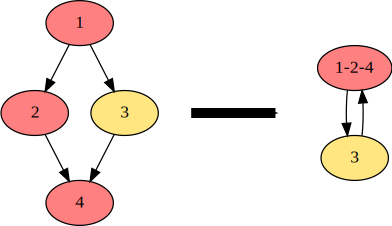
\includegraphics[width=0.4\textwidth]{agg_invalid}
        }%
        \hspace{0.15\textwidth}%
        \subfigure[Agrégation valide]{%
          \label{fig:agg_valid}
          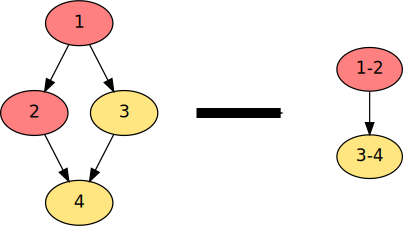
\includegraphics[width=0.4\textwidth]{agg_valid}
        }%
    \end{center}
    \caption{Exemple de deux agrégations, le résultat de \ref{fig:agg_invalid} ne peut pas être ordonnancé à cause du cycle. Le résultat de \ref{fig:agg_valid} peut être ordonnancé mais il n'y a aucun parallélisme à exploiter.}
    \label{fig:agg_basic}
\end{figure}

En premier lieu, nous avons développé une nouvelle interface de programmation en C++, cette interface reprend de Intel TBB le concept d'un objet {\em Tâche} contenant la fonction à exécuter.
%
\`A cela, nous avons ajouté la description des dépendances dans cet objet.
%
Cette interface nous permet de décrire un graphe de tâche complet et de choisir parmi plusieurs ordonnanceurs celui qui ordonnancera le graphe.
%
Avec cette interface, nous pouvons faire des modifications sur le graphe et le rendre plus grossier.
%
Nous avons appelé cette interface Taggre.
%
Grâce à l'utilisation d'heuristiques décrites plus loin dans la thèse, un programme parallèle peut continuer de décrire son parallélisme de façon naturelle, sans se soucier de la granularité.
%
Taggre s'occupera ensuite de faire le travail nécessaire pour rendre ce graphe assez grossier pour qu'un ordonnanceur puisse l'ordonnancer efficacement (Fig.~\ref{fig:coarsening}).

%   (-_-)   %
\begin{figure}[t!]
  \centering
  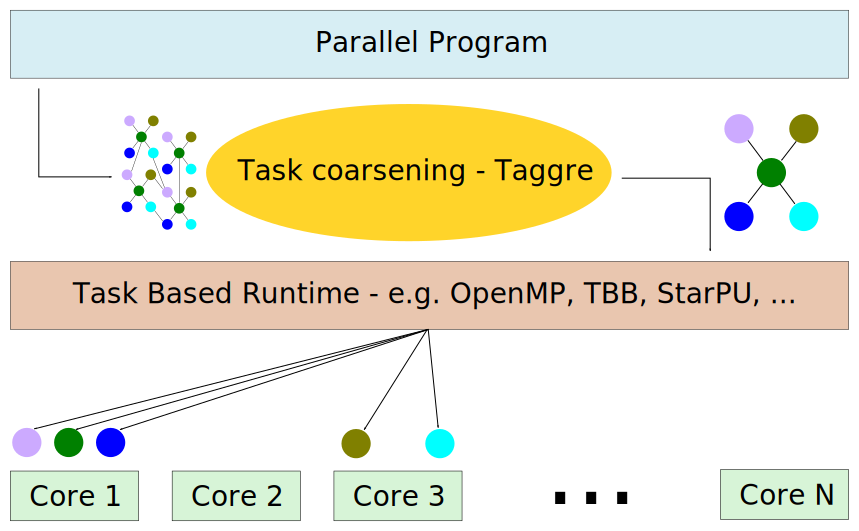
\includegraphics[width=0.8\textwidth]{coarsening}
  \caption{Le programme parallèle fournit un graphe de tâches à Taggre. Taggre modifie le graphe. Taggre fournit le graphe à l'ordonnanceur. Le processus d'agrégation est totalement transparent pour l'ordonnanceur.}
  \label{fig:coarsening}
\end{figure}


\lstinputlisting[inputencoding=utf8/latin1,frame=single,float=t]{src/taggre.cpp}

%-------------------------------
\subsection{Les opérateurs d'agrégations}
Nous appelons {\em opérateurs d'agrégations} les différentes heuristiques utilisées pas Taggre pour grossir un graphe de tâches.
%
Ces heuristiques ont pour règle de garder la propriété acyclique du graphe de tâches.
%
Quatre heuristiques ont été créées, chaque opérateur s'occupe de résoudre un problème spécifique et aucun d'entre eux ne peux créer de cycle.
%
La création d'un cycle lors d'une agrégation intervient lorsque l'on crée un groupe de tâche dans lequel deux des tâches ont une dépendance indirecte, symbolisé par un chemin dans le graphe, et qu'au moins une des tâches de ce chemin n'appartient pas au groupe.


%Pour évaluer l'amélioration apportée par chaque heuristique, nous avons intégré dans Taggre un simulateur minimal qui estimera le temps d'ordonnancement du graphe.
% Les résultats du simulateur minimal ne sont pas bons
%Cette estimation est essentielle dans la mesure où elle permet de mesurer le parallélisme restant pouvant être extrait du graphe grossier.

On pourrait se poser la question de l'utilisation d'un partitionneur de graphe comme opérateur d'agrégation.
%
En effet, les partitionneurs de graphe essaient de créer des groupes de noeud proche spatialement.
%
Si nous prenons en compte ce seul paramètre, ils feraient des opérateurs de très bonne qualité.
%
Malheureusement, les partitionneurs ne travaillent que sur des graphes non orientés.
%
Le résultat de ces opérateurs serait donc inutilisable parce que les graphes obtenus pourraient être composés de cycles.

%-------------------------------
\subsubsection{Séquentiel}
L'opérateur séquentiel, aussi abrégé {\em S} dans Taggre, est un opérateur très simple.
%
Son but est de fusionner les tâches qui n'apportent pas de parallélisme, elles ne font qu'ajouter du surcoût d'ordonnancement au temps total de la simulation.
%
En agrégeant ces tâches ensemble, on ne perd pas de parallélisme et on économise le temps d'ordonnancement des tâches.
%
On peut reconnaître un groupe de deux tâches séquentielles par le fait qu'une des tâches n'a qu'un seul successeur et l'autre tâche n'a qu'un seul prédécesseur (Fig~\ref{fig:algo_S}).


%   (-_-)   %
\begin{figure}[t!]
  \centering
  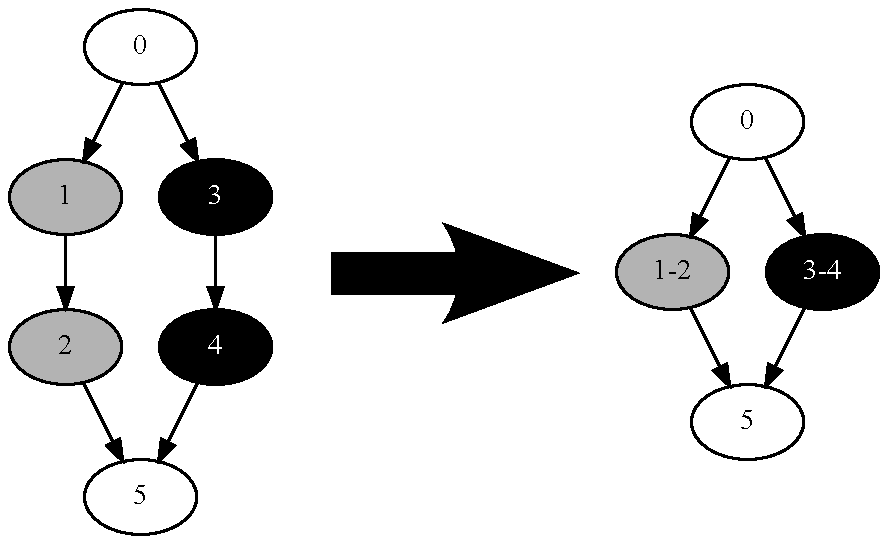
\includegraphics[width=0.6\textwidth]{algo_S}
  \caption{Exemple d'agrégation par l'opérateur séquentiel.}
  \label{fig:algo_S}
\end{figure}

\begin{algorithm}
  \KwData{DAG}
  {\sc Taches} = liste vide \\
  mettre les tâches de DAG dans {\sc Taches} \\
  \While{{\sc Taches} n'est pas vide} {
    {\sc T1} = retirer le premier de {\sc Taches} \\
    \If{Le nombre de successeurs de {\sc T1} == 1} {
      {\sc T2} = premier successeur de {\sc T1} \\
      \If{Le nombre de prédécesseurs de {\sc T2} == 1} {
        {\sc T2} devient {\sc T1} union {\sc T2}\\
      }
    }
  }
  \caption{Algorithme de l'opérateur séquentiel.}
  \label{algo:algo_S}
\end{algorithm}

\subsubsection{Front}
L'opération front, abrégé {\em F} dans Taggre, va limiter le nombre de tâche disponible au même moment dans l'ordonnanceur.
%
Un graphe fournissant énormément de parallélisme par rapport au nombre de coeur disponible n'aura pas forcément un meilleur équilibrage de charge par rapport à un graphe offrant moins de parallélisme.
%
Donc à part congestionner les structures de données servant à maintenir à jour les tâches prêtes à être ordonnancer, il n'est pas nécessaire d'avoir trop de parallélisme dans un graphe.
%
Le parallélisme d'un graphe peut être corréler à sa largeur.
%
En effet, avec un nombre illimité de coeur de calcul, on peut exploiter au mieux le même nombre de coeur que la largeur du graphe.
%
L'algorithme de l'opérateur F consiste à parcourir le graphe par hauteur et de limiter le nombre de tâches par hauteur à un paramètre donné par le programmeur (Fig.~\ref{fig:algo_F2}).
%
Seules les tâches qui ont la même hauteur sont agrégées ensemble, il n'y a donc aucun risque de créer un cycle.
%   (-_-)   %
\begin{figure}[t!]
  \centering
  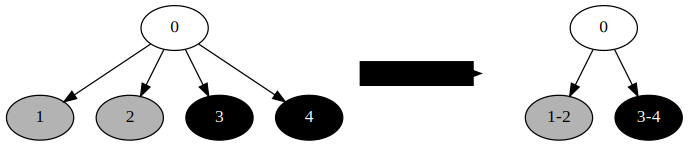
\includegraphics[width=0.7\textwidth]{algo_F2}
  \caption{Exemple d'agrégation avec l'opérateur F et le paramètre 2.}
  \label{fig:algo_F2}
\end{figure}

\subsubsection{Dézoomé}
Je pense qu'il s'agit de l'opérateur le plus intéressant parce qu'il permet d'effectuer des agrégations assez génériques et souvent efficace.
%
Abrégé {\em D} dans Taggre, cet opérateur essaye de créer des groupes de tâches proche spatialement, un peu à la manière d'un partitionneur de graphe.
%
Le nom {\em dézoomé} provient du fait que la structure globale du graphe n'a pas beaucoup changée pendant l'agrégation mais que le nombre de tâches a lui considérablement diminué.
%
Dans les meilleurs cas le nombre de tâches peut être divisé par le paramètre donné par le programmeur (Fig.~\ref{fig:algo_D4}).
%
L'algorithme \ref{algo:algo_D} permet d'implémenter l'opérateur dézoomé tout en assurant l'absence de création de cycle.
%   (-_-)   %
\begin{figure}[t!]
  \centering
  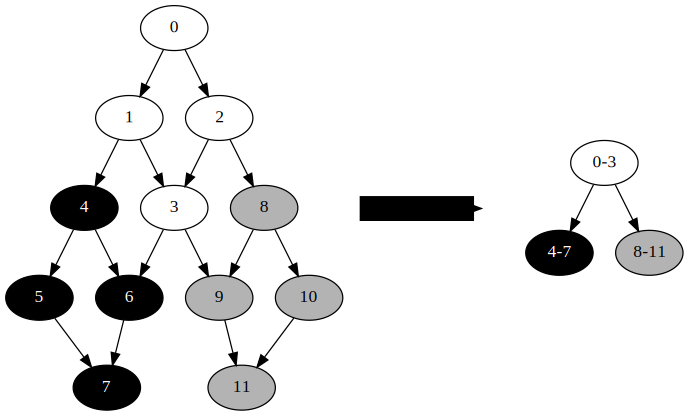
\includegraphics[width=0.8\textwidth]{algo_D4}
  \caption{Exemple d'utilisation de l'opérateur D avec le paramètre 4. Le nombre total de tâche a bien été divisé par 4.}
  \label{fig:algo_D4}
\end{figure}

\begin{algorithm}
  \KwData{$M$, DAG}
  {\sc Prêt} = liste vide \\
  mettre les tâches racines de DAG dans {\sc Prêt} \\
  \While{{\sc Prêt} n'est pas vide} {
    {\sc Profondeur} = {\sc Prêt} \\
    {\sc Prêt} = liste vide \\
    \While{{\sc Profondeur} n'est pas vide} {
      {\sc Maître} = retirer le premier de {\sc Profondeur} \\
      {\sc Release} = liste vide \\
      mettre {\sc Maître} dans {\sc Release} \\
      {\sc Compteur} = 0 \\
      \While{{\sc Compteur} $< M$ {\bf et} {\sc Release} n'est pas vide} {
        {\sc Suivant} = retirer le premier de {\sc Release} \\
        {\sc Compteur}++\\
        agréger {\sc Maître} et {\sc Suivant}\\
        mettre les tâches libérées par {\sc Suivant} dans {\sc Release} \\
        trier {\sc Release} par nombre de précédence de {\sc Maître} \\
      }
      mettre les tâches libérées par {\sc Maître} dans {\sc Profondeur} \\
    }
    mettre les tâches libérées par {\sc Profondeur} dans {\sc Prêt}\\
  }
  \label{algo:algo_D}
  \caption{Opérateur dézoomé.}
\end{algorithm}

\subsubsection{Cube ou continuation}
Cet opérateur a été créé pour être une réponse efficace à nos problèmes.
%
Dans notre cas, le graphe à ordonnancer à exactement la même structure que le réservoir que nous souhaitons modéliser.
%
La plupart du temps, ce modèle sera un cube 3D.
%
En numérotation naturelle et avec un modèle 3D, une bonne agrégation consiste à agréger toutes les tâches d'un axe qui ont les mêmes coordonnées sur les deux autres axes.
%
Cela correspond à {\em aplatir} notre modèle 3D en un modèle 2D (Fig.~\ref{fig:cube5_algo_C}).
%
Par exemple, un cube de 5 éléments de coté, soit 125 tâches, sera transformé en un carré de 5 éléments de coté, soit 25 tâches.


%   (-_-)   %
\begin{figure}[t!]
  \centering
  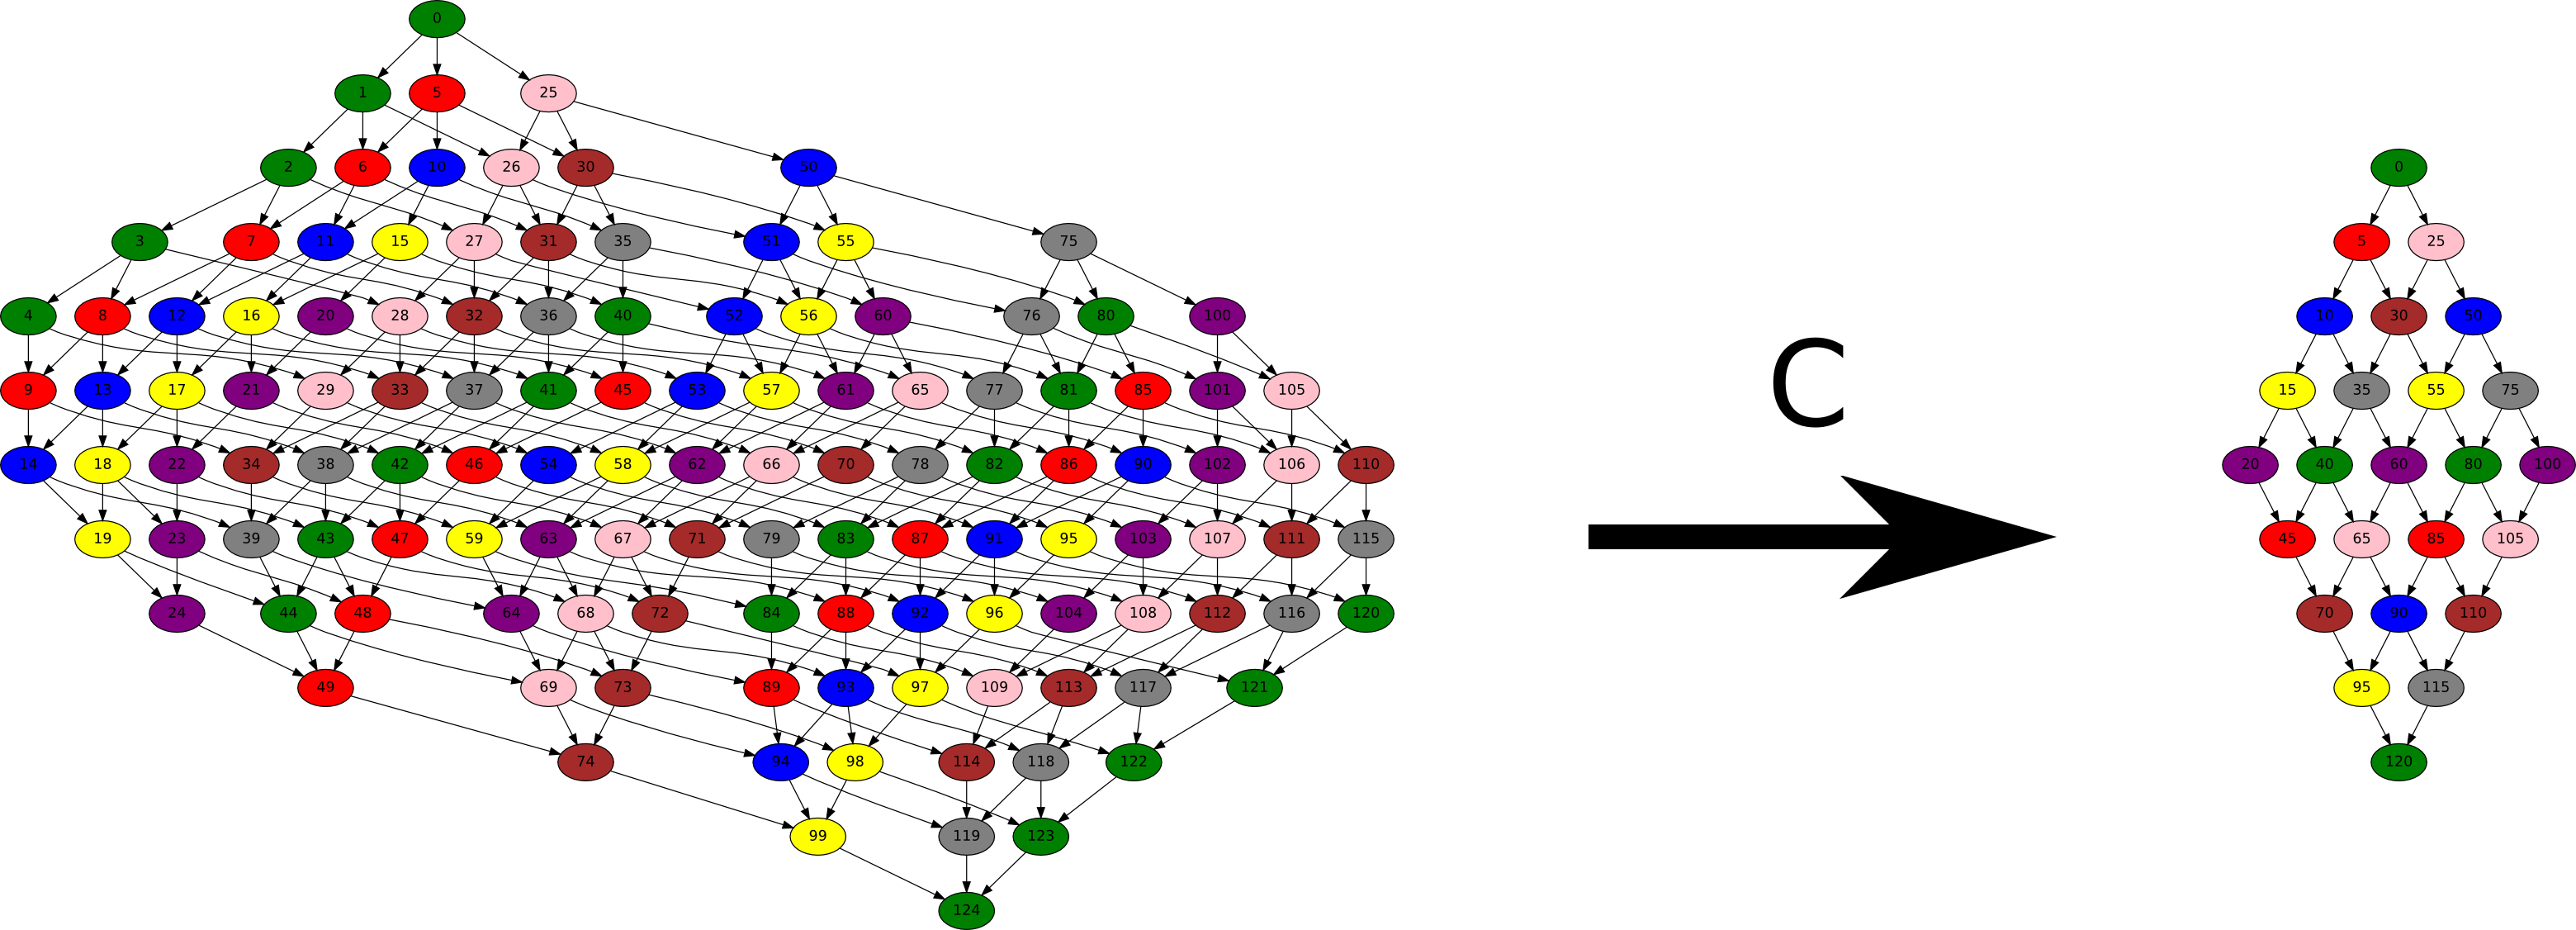
\includegraphics[width=\textwidth]{cube5_operator_c}
  \caption{Exemple d'utilisation de l'opérateur C sur un cube 5x5x5.}
  \label{fig:cube5_algo_C}
\end{figure}


%   (-_-)   %
\begin{figure}[t!]
  \centering
  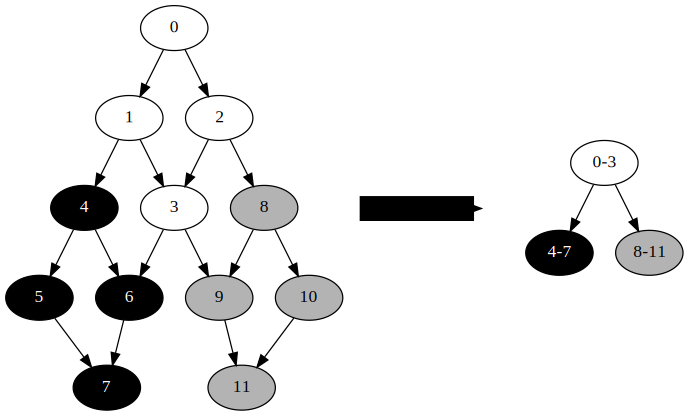
\includegraphics[width=0.8\textwidth]{algo_3}
  \caption{Exemple d'utilisation de l'opérateur C.}
  \label{fig:algo_C}
\end{figure}


Comme pour les autres opérateurs, nous devons vérifier qu'aucun cycle ne sera créé.
%
Pour fonctionner, cet opérateur a besoin que le programmeur attribue un nombre unique à chaque tâche et ainsi avoir un ordre strict sur les tâches.
%
Dans notre cas on va utiliser la numérotation naturelle des cellules.
%
Puis l'opérateur agrégera ensemble les tâches ayant des nombres qui se suivent ainsi qu'une dépendance entre les tâches.
%
Par exemple sur la figure \ref{fig:algo_C} les tâches 2 et 3 ont des nombres consécutifs mais n'ont pas de dépendance entre elles, elles ne seront donc pas agrégées ensemble.


Ajoutons un prédicat à l'algorithme : pour pouvoir utiliser cet algorithme, il faut absolument que pour chaque tâche $i$, l'indice associé à la tâche $i$ soit strictement inférieur aux indices associés aux successeurs de la tâche $i$.
%
Ce prédicat nous permet de s'assurer qu'aucun cycle ne sera créé.
%
En effet, pour créer un cycle avec cet algorithme, il faudrait qu'il existe un chemin entre deux tâches agrégées qui passe par une autre tâche non agrégée.
%
Or, pour agréger une tâche avec une autre, il faut que la différence de leurs indices soit exactement la différence minimale possible dans le graphe.
%
Donc, en prenant en compte le prédicat, si nous agrégeons une tâche T1 avec son successeur T2, il ne peut pas exister de chemin en T1 et T2 passant par une autre tâche.


\begin{algorithm}
  \KwData{DAG}
  {\sc Pas} = Infini \\
  \For{chaque tâche {\sc T1} de DAG} {
    \For{chaque successeurs {\sc T2} de {\sc T1}} {
      \If{indice de {\sc T2} $<=$ indice de {\sc T1}} {
        \Return agrégation impossible
      }

      \If{indice de {\sc T2} - indice de {\sc T1} $<$ {\sc Pas}} {
        {\sc Pas} = indice de {\sc T2} - indice de {\sc T1}
      }
    }
  }

  \For{chaque tâche {\sc T1} de DAG} {
    \For{chaque successeurs {\sc T2} de {\sc T1}} {
      \If{indice de {\sc T2} == indice de {\sc T1} + {\sc Pas}} {
        {\sc T1} devient {\sc T1} union {\sc T2}
      }
    }
  }
  \caption{Algorithme de l'opérateur continuation.}
  \label{algo:algo_C}
\end{algorithm}

%% Dans le cas d'un graphe représentant un cube 3D, cet opérateur fonctionne très bien.
%% %
%% Par contre, dans le cas d'un graphe représentant un carré, il est nécessaire de modifier cette algorithme pour limiter la taille des agrégats tout en optimisant

%-------------------------------
\subsection{Les 13 Dwarfs de berkeley}
Le choix des opérateurs dans Taggre se fait à l'appréciation du programmeur.
%
La collection des {\em 13 nains de Berkeley}\cite{dwarfs} est une méthode de classification des problèmes en fonction de leurs motifs de calculs et de communications.
%
Il est intéressant de voir si Taggre peut répondre aux 13 problèmes et si c'est le cas quelle serait la stratégie d'agrégation à utiliser.
%
Malheureusement, tous les problèmes ne se prêtent pas à cet exercice.
%
Nous avons donc choisi quelques graphes qui peuvent représenter un problème spécifique.


\subsubsection{Méthodes spectrales}
Dans le cas des méthodes spectrales, le graphe représentant le parallélisme est plus large que haut.
%
Le motif du graphe est en papillon, nous avons donc beaucoup de connexion entre chaque hauteur du graphe, l'opérateur F pourras s'occuper de regrouper les tâches d'un même niveau ensemble.
%
Celui-ci nous permettra de diminuer le nombre de tâche en diminuant le parallélisme (Fig.\ref{fig:dwarf_spec}).
%
Pour évaluer le gain lié à l'agrégation, nous allons utiliser le simulateur de Taggre avec les paramètres 0,9 pour les effets caches et 5 pour le coût d'ordonnancement.
%
La hauteur du graphe sera le logarithme en base 2 du nombre de tâches par niveau.
%
La table~\ref{tab:spectral}


%   (-_-)   %
\begin{figure}
  \centering
  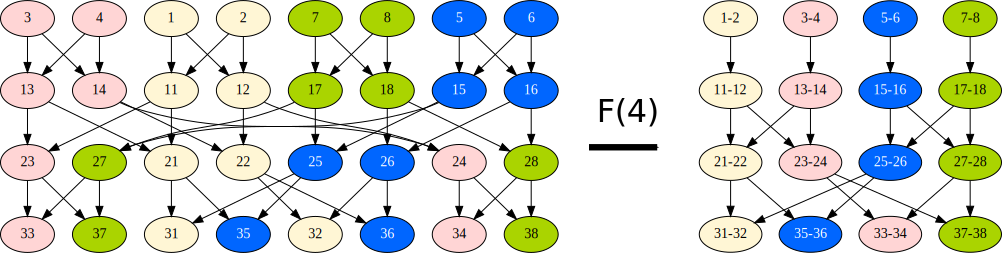
\includegraphics[width=\textwidth]{dwarf_spec}
  \caption{Exemple d'agrégation sur un graphe de méthode spectrale.}
  \label{fig:dwarf_spec}
\end{figure}

%   (-_-)   %
\begin{center}
  \begin{tabular}{|l|c|c|c|c|c|c|c|c|}
    \hline
   Nombre de tâches &  \multicolumn{8}{c|}{Types d'agrégations}\\
   par niveau & \O & F(6) & F(12) & F(24) & D(8) & D(16) & D(32) & D(64) \\
    \hline
   32768 & 262146 & 108246 & 51714 & 39487 & 70425 & 55788 & 40980 & 46409 \\
   1024  & 1690 & 2162 & 937 & 903 & 1035 & 965 & 899 & 1033 \\
    \hline
  \end{tabular}
  \captionof{table}{Résultats du simulateur d'exécution de tâches sur un graphe typique des méthodes spectrales.}
  \label{tab:spectral}
\end{center}

%% RES 15 niveau
%% 0    262146
%% F 12 51714.9
%% F 24 39487.8
%% F 6  108246
%% D 8  70425
%% D 16 55788.5
%% D 32 40980
%% D 64 46409.6

%% RES 10 niveau
%% 0    1690
%% F 12 937
%% F 24 903
%% F 6  2162
%% D 8  1035
%% D 16 965
%% D 32 899
%% D 64 1033
\subsubsection{Les arbres}

%+++++++++++++++++++++++++++++++




%+++++++++++++++++++++++++++++++
\section{Résultats}
%-------------------------------
\subsection{Amélioration de la factorisation et de la résolution triangulaire}
Dans un premier temps, nous allons nous consacrer à l'amélioration de la parallélisation de la factorisation ILU(k).
%
Chaque tâche du graphe de tâches représente la factorisation d'une ligne de la matrice.
%
Cette granularité est trop fine, mais c'est voulu, elle représente la granularité que nous obtenons en décrivant naturellement l'algorithme de la factorisation.
%
Nous avons choisi de simuler deux réservoirs, un cube généré de taille 80 cellules de côté et le réservoir SPE10.
%
Dans le cas du cube, il est possible de choisir le nombre de variables primaires utilisées dans le calcul.
%
Pour rappel, le nombre de variables primaires correspond au nombre de composants simulés.
%
Chaque entrée non-nulle de la matrice correspond à l'interaction entre 2 cellules et sera composée d'une petite matrice dense $Npri*Npri$ avec $Npri$ le nombre de variables primaires.
%
Nous avons choisi de simuler le cube avec 1 variable primaire, 3 variables primaires (modèle {\em black-oil}) et 8 variables primaires (modèle {\em compositionnel}).
%
Pour le réservoir SPE10, c'est un cas {\em black-oil} à 3 variables primaires.
%
Au final nous avons donc 4 matrices différentes.
%
Nous ne faisons pas varier la taille du cube, car les résultats obtenus avec des cubes générés de tailles raisonnablement différentes sont équivalents.

\subsubsection{Sans agrégation}
Nous avons utilisé OpenMP pour tester la parallélisation à grain fin sans agrégation.
%
OpenMP 3.0 n'ayant pas de gestion de dépendances entre les tâches, nous utiliserons un système de décrémentation atomique.
%
Comme le montrent les résultats de la figure~\ref{fig:res_facto_no_agg}, le nombre de variables primaires a une importance considérable sur les performances que nous obtenons.
%
L'utilisation de 2 threads n'est viable que dans le cas où nous utilisons 8 variables primaires.
%
Dans les autres cas, même en utilisant 4 threads, nous perdons du temps.
%
Ici, le nombre de variables primaires va définir le nombre d'opérations faites par ligne de la matrice, donc plus ce nombre est grand, plus il y aura de travail à faire.
%
Ces résultats confirment notre problème de granularité.
%
Au final, avec l'utilisation des 12 coeurs de calcul de la machine, nous obtenons des accélérations plutôt décevantes, par exemple, pour les cas à 3 variables primaires, le code tourne environ 2,5 fois plus vite que la version séquentielle, mais il utilise 12 fois plus de puissance de calcul.

%   (-_-)   %
\begin{figure}[!h]
  \centering
  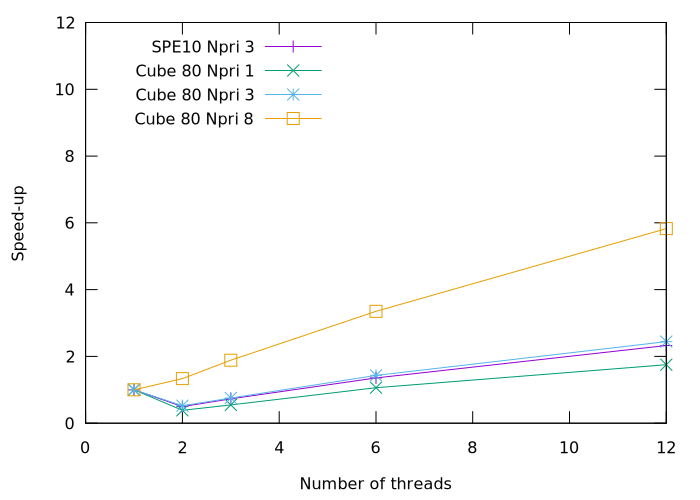
\includegraphics[width=0.7\textwidth]{res_facto_no_agg}
  \caption{Performance de la factorisation sur 12 coeurs sans utiliser Taggre.}
  \label{fig:res_facto_no_agg}
\end{figure}


\subsubsection{Avec l'opérateur F}
Dans un premier temps, nous allons appliquer l'opérateur F avec le paramètre 36.
%
Cet opérateur va donc limiter la largeur du graphe pour qu'il y ait au plus 36 tâches par hauteur du graphe.
%
Nous aurons donc 3 fois plus de tâches que de coeurs de calcul, cela permet de diminuer fortement le nombre de tâches tout en gardant assez de parallélisme pour avoir un bon équilibrage de charge.
%
Nous réduisons donc le parallélisme, mais nous réduisons aussi le nombre de tâches, on divise par 62 le nombre de tâches pour un cube de 80 de côté, nous passons de 512000 tâches à 8232 tâches.
%
Pour le cas SPE10, le nombre de tâches passe de 1094421 à 12896 soit 84 fois moins de tâches.
%
La figure~\ref{fig:res_facto_f36} nous montre une amélioration du temps de factorisation quand le nombre de variables primaires est faible.
%
Cela vient du fait que le surcoût d'ordonnancement de la tâche est du même ordre de grandeur que le temps de calcul de la tâche.
%
Avec 3 variables primaires, la factorisation est 30~\% plus rapide.
%
Avec 1 variable primaire, le temps de factorisation est divisé par 2.
%
Dans le cas où le nombre de variables primaires est élevé, il n'y a pas beaucoup d'amélioration (6~\%).
%
Ici, cet opérateur ne permet pas d'optimiser les accès mémoire caches, seul le surcoût d'ordonnancement est réduit.

%   (-_-)   %
\begin{figure}[!h]
  \centering
  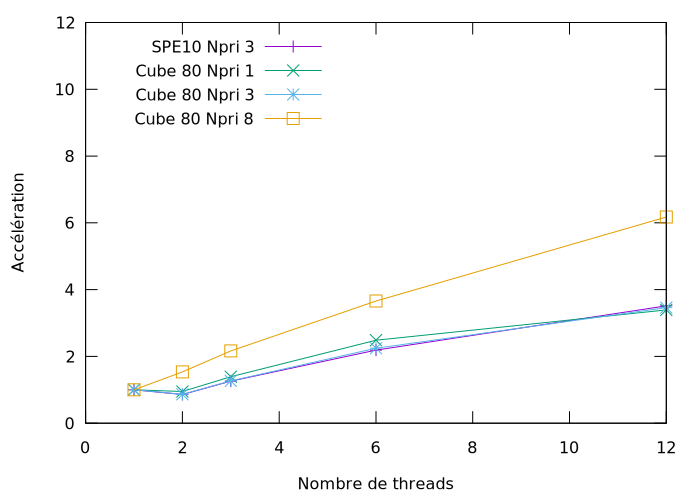
\includegraphics[width=0.7\textwidth]{res_facto_f36}
  \caption{Performance de la factorisation sur 12 coeurs avec Taggre F(36).}
  \label{fig:res_facto_f36}
\end{figure}


\subsubsection{Avec l'opérateur D}
Essayons maintenant l'opérateur D avec le paramètre 8.
%
Cet opérateur va essayer de créer des groupes de 8 tâches assez proches dans le graphe.
%
Nous allons donc diviser par 8 le nombre de tâches, passant ainsi de 512000 tâches à 64000 tâches.
%
Ce qui peut paraître peu mais cette valeur a été choisie empiriquement parmi un ensemble de valeurs.
%
Les autres valeurs donnent des résultats légèrement moins bons, par exemple le paramètre 4 offre une accélération de 3,35, tandis que le paramètre 12 offre 3,55 et finalement le paramètre 8 offre une accélération de 3,72.
%
Comparé à l'opérateur F, il y a très peu d'amélioration quand le nombre de variables primaires est faible (Fig.~\ref{fig:res_facto_d8}).
%
Par contre, avec 8 variables primaires, on obtient un gain de performance qui est dû à une meilleure utilisation des caches, surtout du cache L2 avec une diminution de 10\% des défauts de cache d'après les compteurs matériels du processeur (Tab.~\ref{tab:cache_miss}).


%   (-_-)   %
\begin{figure}[!h]
  \centering
  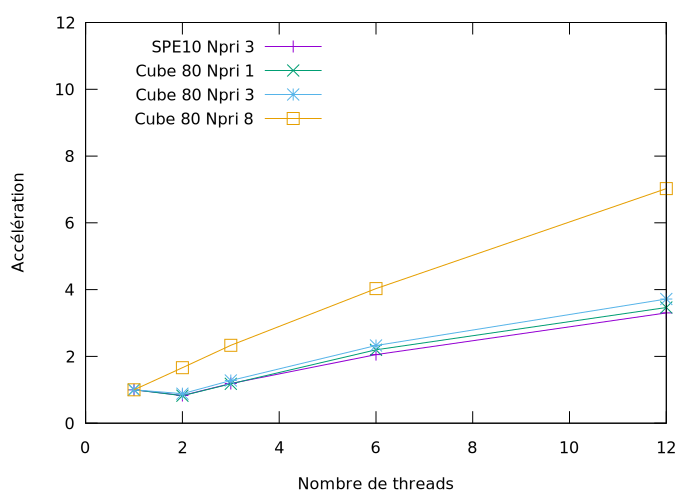
\includegraphics[width=0.7\textwidth]{res_facto_d8}
  \caption{Performance de la factorisation sur 12 coeurs avec Taggre D(8).}
  \label{fig:res_facto_d8}
\end{figure}


\subsubsection{Avec l'opérateur C}
Les deux précédents opérateurs donnent déjà des résultats, mais nous pensons que le meilleur opérateur pour nos matrices reste l'opérateur C.
%
Il a l'avantage de réduire grandement le nombre de tâches comme l'opérateur F et il forme des groupes de tâches permettant une meilleure réutilisation des données en cache.
%
Par contre, il se pourrait que le parallélisme en pâtisse.
%
Comme le montrent les résultats de la figure~\ref{fig:res_facto_c}, tous les cas tests sont améliorés.
%
Il y a bien deux grandes améliorations : la réduction du nombre de tâches et une meilleure réutilisation des caches.
%
Comme pour tous les opérateurs, le nombre de tâches a été réduit, mais dans ce cas la réduction est bien plus importante.
%
Par contre, l'amélioration des effets caches est bien meilleure que dans les autres opérateurs, nous obtenons une diminution de 25\% des défauts de cache des niveaux 1 et 2 par rapport à l'opérateur F.
%
Cette amélioration est inexistante dans le cas de l'opérateur F, les tâches agrégées n'avaient pas une bonne réutilisabilité des données en cache.
%
Au contraire, l'opérateur D ne réduisait que de très peu le nombre de tâches, mais améliorait la réutilisation des caches.
%
L'opérateur C offre donc le meilleur des deux opérateurs, il produit peu de tâches et en plus ces tâches réutilisent correctement les données en cache.
% L2 stats : F:1.10, D:0.96, C:0.87

%   (-_-)   %
\begin{figure}[!h]
  \centering
  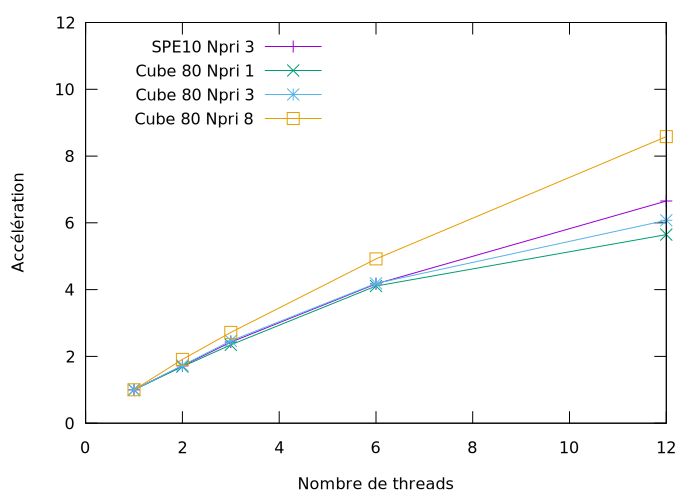
\includegraphics[width=0.7\textwidth]{res_facto_c}
  \caption{Performance de la factorisation sur 12 coeurs avec Taggre C.}
  \label{fig:res_facto_c}
\end{figure}

\subsubsection{Avec plusieurs opérateurs}
Il est aussi possible de combiner plusieurs opérateurs, sur la figure~\ref{fig:res_facto_cd2} nous avons combiné l'opérateur C avec l'opérateur D(2).
%
On observe un très léger gain de performance quand on a une seule variable primaire, mais dans les autres cas on observe le contraire.
%
Le premier opérateur améliore déjà les effets cache et augmente suffisamment la taille des tâches pour obtenir de bonnes performances, il n'y a donc presque plus d'améliorations possibles.
%
Malgré ces optimisations, nous n'atteignons pas une accélération parfaite, avec au mieux une accélération de 8,7 pour 12 coeurs.
%
Ce souci de performance est lié à l'architecture mémoire de la machine, nous donnerons plus d'explication dans la partie suivante de la thèse.


%   (-_-)   %
\begin{figure}[!h]
  \centering
  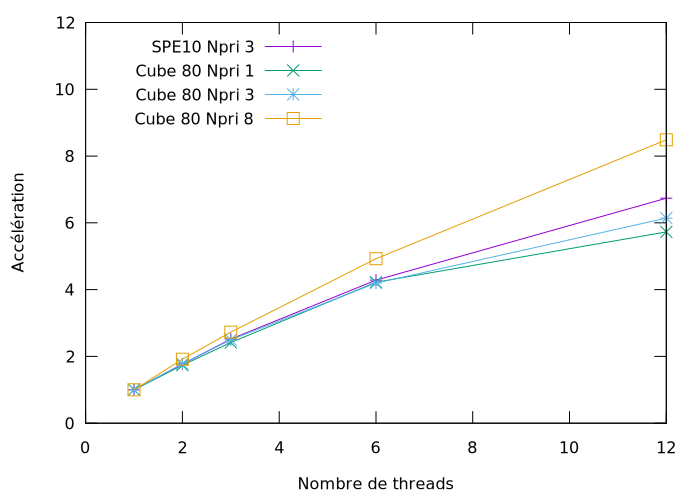
\includegraphics[width=0.7\textwidth]{res_facto_cd2}
  \caption{Performance de la factorisation sur 12 coeurs avec Taggre CD(2).}
  \label{fig:res_facto_cd2}
\end{figure}
\subsubsection{En résumé}

%   (-_-)   %
\begin{center}
  \begin{tabular}{|r|c|c|c|c|c|c|c|c|c|c|}
    \hline
    Type de  &  \multicolumn{5}{c|}{Accélération}  &  \multicolumn{5}{c|}{Nombre de tâches} \\
    matrice  &  \O & F(36) & D(8) & C & CD(2)  &  \O & F(36) & D(8) & C & CD(2)\\
    \hline
    Cube 80 Npri 1 & 1,75 & 3,39 & 3.46 & 5.65 & 5.73 & 512000  & 8232  & 64000  & 6400  & 3200 \\
    Cube 80 Npri 3 & 2,44 & 3,46 & 3.72 & 6.07 & 6.14 & 512000  & 8232  & 64000  & 6400  & 3200 \\
    Cube 80 Npri 8 & 5,83 & 6,17 & 7.02 & 8.58 & 8.48 & 512000  & 8232  & 64000  & 6400  & 3200 \\
    SPE10 Npri 3   & 2,32 & 3,52 & 3.30 & 6.65 & 6.73 & 1094421 & 12896 & 136887 & 36281 & 18181 \\
    \hline
  \end{tabular}
  \captionof{table}{Récapitulatif des résultats de la factorisation sur 12 coeurs de calcul suivant les opérateurs appliqués.}
  \label{tab:facto_res}
\end{center}

%   (-_-)   %
\begin{center}
  \begin{tabular}{|r|c|c|c|}
    \hline
                & Cache L1 & Cache L2 & Cache L3 \\
    \hline
    Opérateur F &   0.009  &  1.102   &  0.096 \\
    Opérateur D &   0.009  &  0.966   &  0.092 \\
    Opérateur C &   0.007  &  0.873   &  0.091 \\
    \hline
  \end{tabular}
  \captionof{table}{Ratio du nombre de requêtes caches qui ont échouées par rapport au nombre de requêtes qui ont été faites. Résultats des compteurs matériels obtenues avec Likwid.}
  \label{tab:cache_miss}
\end{center}

\subsubsection{Résultats de la résolution triangulaire}
Essayons maintenant cette technique sur la partie résolution triangulaire du code.
%
Les performances sans agrégation sont bien en dessous de la partie factorisation (Fig.~\ref{fig:res_trsv_no_agg}).
%
Même en utilisant 12 threads, seule la version avec 8 variables primaires donne de meilleurs résultats que la version séquentielle.
%
Encore une fois, il s'agit d'un problème de granularité, le graphe à ordonnancer est le même que pour la factorisation, mais les tâches sont plus petites.

%   (-_-)   %
\begin{figure}[!h]
  \centering
  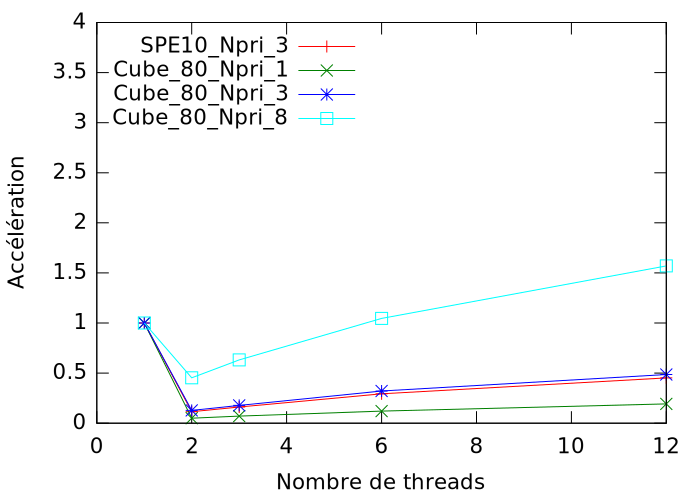
\includegraphics[width=0.7\textwidth]{res_trsv_no_agg}
  \caption{Performance de la résolution triangulaire sur 12 coeurs sans utiliser Taggre.}
  \label{fig:res_trsv_no_agg}
\end{figure}

Si nous regardons les résultats avec la meilleure agrégation que nous ayons, l'agrégation CD(2), on obtient des résultats légèrement meilleurs, mais on n'est encore loin de l'accélération parfaite (Fig.~\ref{fig:res_trsv_cd2}).
%
On arrive ici aux limites de notre méthode, la granularité n'est pas encore suffisante pour permettre d'obtenir de très bonnes performances.
%
Mais si nous augmentons encore la granularité, il n'y aura plus assez de parallélisme pour avoir un bon équilibrage de charge et le temps final sera supérieur.

%   (-_-)   %
\begin{figure}[!h]
  \centering
  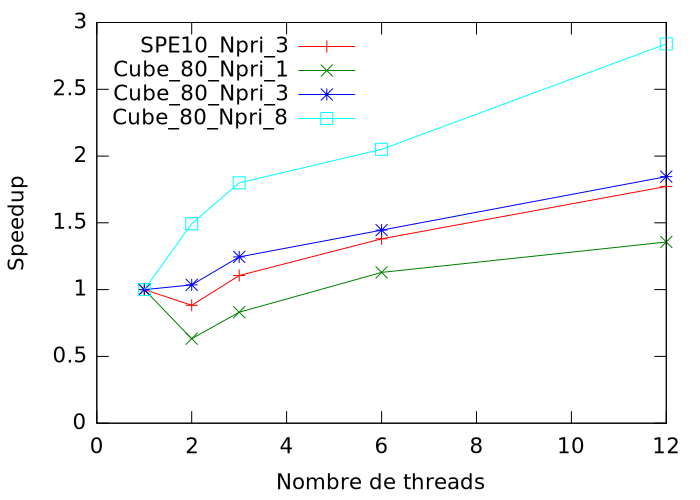
\includegraphics[width=0.7\textwidth]{res_trsv_cd2}
  \caption{Performance de la résolution triangulaire sur 12 coeurs avec Taggre CD(2).}
  \label{fig:res_trsv_cd2}
\end{figure}




%% +---------------------------+-------------+-------------+-------------+------------+
%% |          Metric           |     Sum     |     Max     |     Min     |    Avg     |
%% +---------------------------+-------------+-------------+-------------+------------+
%% | Runtime (RDTSC) [s] STAT  |   1923.94   |   160.328   |   160.328   |  160.328   |
%% | Runtime unhalted [s] STAT |   1870.36   |   160.82    |   152.347   |  155.864   |
%% |     Clock [MHz] STAT      |   34528.4   |   2906.13   |   2850.24   |  2877.37   |
%% |         CPI STAT          |   1.03608   |   1.04174   |   1.02468   | 0.0863398  |
%% |  Data cache misses STAT   | 4.59444e+10 | 4.08753e+09 | 3.71715e+09 | 3.8287e+09 |
%% | Data cache miss rate STAT |   0.10934   | 0.00932521  | 0.00905509  | 0.0091117  |
%% +---------------------------+-------------+-------------+-------------+------------+
%% +---------------------------+-------------+-------------+-------------+-------------+
%% |          Metric           |     Sum     |     Max     |     Min     |     Avg     |
%% +---------------------------+-------------+-------------+-------------+-------------+
%% | Runtime (RDTSC) [s] STAT  |   2004.24   |   167.02    |   167.02    |   167.02    |
%% | Runtime unhalted [s] STAT |   2061.97   |   175.567   |   170.297   |   171.831   |
%% |     Clock [MHz] STAT      |   36151.6   |   3017.39   |   3008.02   |   3012.64   |
%% |         CPI STAT          |   1.14231   |   1.14711   |   1.13205   |  0.0951929  |
%% |  Data cache misses STAT   | 4.87067e+10 | 4.29088e+09 | 4.00937e+09 | 4.05889e+09 |
%% | Data cache miss rate STAT |  0.115926   | 0.00990628  | 0.00962271  | 0.00966052  |
%% +---------------------------+-------------+-------------+-------------+-------------+
%% +---------------------------+-------------+-------------+-------------+-------------+
%% |          Metric           |     Sum     |     Max     |     Min     |     Avg     |
%% +---------------------------+-------------+-------------+-------------+-------------+
%% | Runtime (RDTSC) [s] STAT  |   1640.85   |   136.737   |   136.737   |   136.737   |
%% | Runtime unhalted [s] STAT |   1686.77   |   144.388   |   138.353   |   140.564   |
%% |     Clock [MHz] STAT      |   36255.7   |   3046.34   |   2998.08   |   3021.31   |
%% |         CPI STAT          |  0.934931   |  0.937527   |  0.926718   |  0.0779109  |
%% |  Data cache misses STAT   | 3.85951e+10 | 3.43628e+09 | 3.14135e+09 | 3.21626e+09 |
%% | Data cache miss rate STAT |  0.0919074  | 0.00789712  | 0.00762214  | 0.00765895  |
%% +---------------------------+-------------+-------------+-------------+-------------+


%% +---------------------------+----------+-----------+-----------+-----------+
%% |          Metric           |   Sum    |    Max    |    Min    |    Avg    |
%% +---------------------------+----------+-----------+-----------+-----------+
%% | Runtime (RDTSC) [s] STAT  | 2013.52  |  167.794  |  167.794  |  167.794  |
%% | Runtime unhalted [s] STAT |  2049.5  |  173.386  |  167.781  |  170.792  |
%% |     Clock [MHz] STAT      | 35861.8  |  3005.94  |  2972.33  |  2988.48  |
%% |         CPI STAT          | 1.13698  |  1.14624  |  1.12814  | 0.0947487 |
%% |   L2 request rate STAT    | 0.139712 | 0.0119216 | 0.0115742 | 0.0116426 |
%% |     L2 miss rate STAT     | 0.154052 | 0.0129583 | 0.0127815 | 0.0128376 |
%% |    L2 miss ratio STAT     | 13.2323  |  1.10948  |  1.08696  |  1.10269  |
%% +---------------------------+----------+-----------+-----------+-----------+
%% +---------------------------+----------+-----------+-----------+-----------+
%% |          Metric           |   Sum    |    Max    |    Min    |    Avg    |
%% +---------------------------+----------+-----------+-----------+-----------+
%% | Runtime (RDTSC) [s] STAT  | 1966.96  |  163.913  |  163.913  |  163.913  |
%% | Runtime unhalted [s] STAT | 1886.06  |  158.261  |  156.494  |  157.172  |
%% |     Clock [MHz] STAT      | 34326.8  |  2883.42  |  2837.74  |  2860.57  |
%% |         CPI STAT          | 1.03718  |  1.06006  |  1.01601  | 0.0864318 |
%% |   L2 request rate STAT    | 0.152488 | 0.0130698 | 0.0125945 | 0.0127073 |
%% |     L2 miss rate STAT     | 0.14729  | 0.0125144 | 0.0121436 | 0.0122742 |
%% |    L2 miss ratio STAT     | 11.5912  | 0.970545  | 0.957504  | 0.965933  |
%% +---------------------------+----------+-----------+-----------+-----------+
%% +---------------------------+----------+-----------+-----------+-----------+
%% |          Metric           |   Sum    |    Max    |    Min    |    Avg    |
%% +---------------------------+----------+-----------+-----------+-----------+
%% | Runtime (RDTSC) [s] STAT  |  1652.6  |  137.716  |  137.716  |  137.716  |
%% | Runtime unhalted [s] STAT | 1694.79  |  142.824  |  140.196  |  141.233  |
%% |     Clock [MHz] STAT      | 36166.7  |  3035.99  |  2993.16  |  3013.9   |
%% |         CPI STAT          | 0.937105 | 0.962554  | 0.921956  | 0.0780921 |
%% |   L2 request rate STAT    | 0.158081 | 0.0134666 | 0.0131121 | 0.0131734 |
%% |     L2 miss rate STAT     | 0.138087 | 0.0116948 | 0.0114514 | 0.0115072 |
%% |    L2 miss ratio STAT     | 10.4823  |  0.87775  |  0.86843  | 0.873526  |
%% +---------------------------+----------+-----------+-----------+-----------+

%% +---------------------------+----------+-----------+---------+------------+
%% |          Metric           |   Sum    |    Max    |   Min   |    Avg     |
%% +---------------------------+----------+-----------+---------+------------+
%% | Runtime (RDTSC) [s] STAT  | 2014.07  |  167.839  | 167.839 |  167.839   |
%% | Runtime unhalted [s] STAT | 2045.66  |  172.625  | 168.205 |  170.471   |
%% |     Clock [MHz] STAT      | 35826.2  |  3000.16  | 2971.72 |  2985.52   |
%% |         CPI STAT          | 1.13743  |  1.14473  | 1.12957 | 0.0947856  |
%% |   L3 request rate STAT    | 0.085237 | 0.0429422 |    0    | 0.00710308 |
%% |     L3 miss rate STAT     | 0.116483 | 0.0586274 |    0    | 0.00970692 |
%% |    L3 miss ratio STAT     |  1.1549  | 0.577687  |    0    | 0.0962418  |
%% +---------------------------+----------+-----------+---------+------------+
%% +---------------------------+-----------+-----------+---------+------------+
%% |          Metric           |    Sum    |    Max    |   Min   |    Avg     |
%% +---------------------------+-----------+-----------+---------+------------+
%% | Runtime (RDTSC) [s] STAT  |  1932.6   |  161.05   | 161.05  |   161.05   |
%% | Runtime unhalted [s] STAT |  1869.75  |  159.171  | 152.621 |  155.813   |
%% |     Clock [MHz] STAT      |  34423.7  |  2896.06  | 2841.43 |  2868.64   |
%% |         CPI STAT          |  1.03599  |  1.03868  | 1.03237 | 0.0863323  |
%% |   L3 request rate STAT    | 0.0858767 | 0.0432998 |    0    | 0.00715639 |
%% |     L3 miss rate STAT     | 0.106569  | 0.0534681 |    0    | 0.00888075 |
%% |    L3 miss ratio STAT     |  1.10754  | 0.554997  |    0    | 0.0922947  |
%% +---------------------------+-----------+-----------+---------+------------+
%% +---------------------------+-----------+-----------+----------+------------+
%% |          Metric           |    Sum    |    Max    |   Min    |    Avg     |
%% +---------------------------+-----------+-----------+----------+------------+
%% | Runtime (RDTSC) [s] STAT  |  1696.46  |  141.372  | 141.372  |  141.372   |
%% | Runtime unhalted [s] STAT |  1699.84  |  146.474  | 137.316  |  141.654   |
%% |     Clock [MHz] STAT      |  35865.4  |  3011.87  | 2965.87  |  2988.79   |
%% |         CPI STAT          | 0.931982  | 0.946119  | 0.924821 | 0.0776651  |
%% |   L3 request rate STAT    | 0.0785352 | 0.0400494 |    0     | 0.0065446  |
%% |     L3 miss rate STAT     | 0.0962549 | 0.0481313 |    0     | 0.00802125 |
%% |    L3 miss ratio STAT     |  1.10147  |  0.55564  |    0     | 0.0917888  |
%% +---------------------------+-----------+-----------+----------+------------+

%% +---------------------------------+------------+-------------+-------------+-------------+
%% |             Metric              |    Sum     |     Max     |     Min     |     Avg     |
%% +---------------------------------+------------+-------------+-------------+-------------+
%% |    Runtime (RDTSC) [s] STAT     |  2070.55   |   172.546   |   172.546   |   172.546   |
%% |    Runtime unhalted [s] STAT    |  2068.93   |   175.779   |   169.669   |   172.411   |
%% |        Clock [MHz] STAT         |  35538.6   |   3007.39   |   2915.92   |   2961.55   |
%% |            CPI STAT             |  1.13513   |   1.15526   |   1.11284   |  0.094594   |
%% |        Branch rate STAT         |  0.905246  |  0.0790124  |  0.0746446  |  0.0754372  |
%% | Branch misprediction rate STAT  | 0.00516248 | 0.000476814 | 0.000405921 | 0.000430207 |
%% | Branch misprediction ratio STAT | 0.0684119  | 0.00618842  | 0.00543805  | 0.00570099  |
%% |  Instructions per branch STAT   |  159.109   |   13.3968   |   12.6562   |   13.2591   |
%% +---------------------------------+------------+-------------+-------------+-------------+
%% +---------------------------------+------------+-------------+-------------+-------------+
%% |             Metric              |    Sum     |     Max     |     Min     |     Avg     |
%% +---------------------------------+------------+-------------+-------------+-------------+
%% |    Runtime (RDTSC) [s] STAT     |  1961.67   |   163.472   |   163.472   |   163.472   |
%% |    Runtime unhalted [s] STAT    |  1876.49   |   158.39    |   154.522   |   156.374   |
%% |        Clock [MHz] STAT         |  34367.1   |   2882.84   |   2844.95   |   2863.92   |
%% |            CPI STAT             |   1.0338   |   1.05326   |   1.01697   |  0.0861503  |
%% |        Branch rate STAT         |  0.897154  |  0.0761396  |  0.0736554  |  0.0747628  |
%% | Branch misprediction rate STAT  | 0.00511161 | 0.000463287 | 0.000395029 | 0.000425968 |
%% | Branch misprediction ratio STAT | 0.0683374  | 0.00613752  | 0.00536154  | 0.00569478  |
%% |  Instructions per branch STAT   |  160.529   |   13.5767   |   13.1338   |   13.3774   |
%% +---------------------------------+------------+-------------+-------------+-------------+



%% +---------------------------+---------+---------+---------+-----------+
%% |          Metric           |   Sum   |   Max   |   Min   |    Avg    |
%% +---------------------------+---------+---------+---------+-----------+
%% | Runtime (RDTSC) [s] STAT  | 1961.79 | 163.482 | 163.482 |  163.482  |
%% | Runtime unhalted [s] STAT | 1874.13 | 160.463 | 152.47  |  156.177  |
%% |     Clock [MHz] STAT      | 34317.2 | 2879.83 | 2839.8  |  2859.77  |
%% |         CPI STAT          | 1.0348  | 1.05031 | 1.02074 | 0.0862334 |
%% | Load to Store ratio STAT  | 44.4467 | 3.72245 | 3.6765  |  3.70389  |
%% +---------------------------+---------+---------+---------+-----------+

%-------------------------------
\subsection{Surcoût d'agrégation}
L'application des opérateurs d'agrégation a un surcoût.
%
Il est nécessaire de savoir à partir de quel moment le surcoût d'agrégation devient plus petit que le temps gagné par l'agrégation.
%
Dans notre cas l'agrégation est faite au début du programme et reste valide tant que la structure du réservoir ne change pas.
%
Le temps passé à appliquer les opérateurs d'agrégation va dépendre du nombre de tâche, des opérateurs et de l'ordre des opérateurs.
%
L'opérateur C mettra 150~$\mu{s}$ a traiter une tâche, l'opérateur F mettra 190~$\mu{s}$ et l'opérateur D mettra 250~$\mu{s}$.
%
Par exemple pour la matrice SPE10 il faut 1,67~s pour appliquer l'opérateur C, 2,94~s pour appliquer l'opérateur D(8) et 2.19s pour appliquer CD(2).
%
Toujours pour le cas SPE10, il devient rentable d'utiliser Taggre à partir d'environ 8 factorisations ou 10 résolutions triangulaires (Tab.~\ref{tab:gain_agg}).
%
Les 10 résolutions triangulaires peuvent être faites dans une résolution du GMRES.

%   (-_-)   %
\begin{center}
  \begin{tabular}{ | r | c || c | c | c | }
    \hline
    Matrice & Agrégation & Temps agrégation & Gain factorisation & Gain résolution \\
    \hline
    \hline
    SPE10   &      C     & 1,67          & 0,188          & 0,171 \\
    \hline
    SPE10   &    D(8)    & 2,94          & 0,087          & 0,124 \\
    \hline
    SPE10   &    CD(2)   & 2,19          & 0,189          & 0.173 \\
    \hline
    \hline
    Cube 100&      C     & 1,49          & 0,167          & 0,163 \\
    \hline
    Cube 100&    D(8)    & 2,52          & 0,095          & 0,132 \\
    \hline
    Cube 100&    CD(2)   & 2,52          & 0,167          & 0,165 \\
    \hline
  \end{tabular}
  \captionof{table}{Temps d'application des opérateurs d'agrégation et les gains de temps obtenus sur les opérations d'algèbre linéaire.}
  \label{tab:gain_agg}
\end{center}

%-------------------------------
\subsection{Méthode de Jacobi par blocs}
Afin d'obtenir une évaluation de la borne maximale de l'accélération qu'il est possible d'obtenir sur une machine donnée, nous proposons de connaître l'accélération obtenue par une méthode de Jacobi par blocs et de la comparer à notre solution.
%
Dans cette méthode, nous considérons le cas où chaque coeur effectue la factorisation ILU d'un sous bloc diagonal de la matrice.
%
Cette méthode de préconditionnement induit une factorisation et une résolution triangulaire totalement indépendante sur chaque coeur.
%
Elle n'est évidemment pas équivalente numériquement à effectuer une factorisation ILU de toute la matrice.
%
Plus on utilise de coeurs, plus ce préconditionneur est inefficace numériquement\cite{domain_decomp}.
%
Mais l'intérêt cette évaluation est que l'accélération obtenue donne une borne supérieure de l'accélération de la factorisation ILU sur la matrice complète.
%
Cette borne existe puisqu’individuellement chaque coeur utilise une factorisation dont la bande passante mémoire est approximativement égale à celle de l'algorithme ILU globale.
%
Malgré un parallélisme idéal, nous n'obtenons pas une accélération parfaite (Fig.~\ref{fig:res_facto_mpi}).
%
C'est un problème que l'on rencontre souvent dans les codes d'algèbre linéaire creuse.
%
Si l'on compare les accélérations obtenues avec celles obtenues avec l'agrégation de tâches, on peut voir des résultats légèrement meilleurs pour la méthode Jacobi par blocs.
%
Notre solution d'agrégation n'est pas optimale, mais cette différence d'accélération n'est pas seulement due à la granularité du calcul.

%   (-_-)   %
\begin{figure}
  \centering
  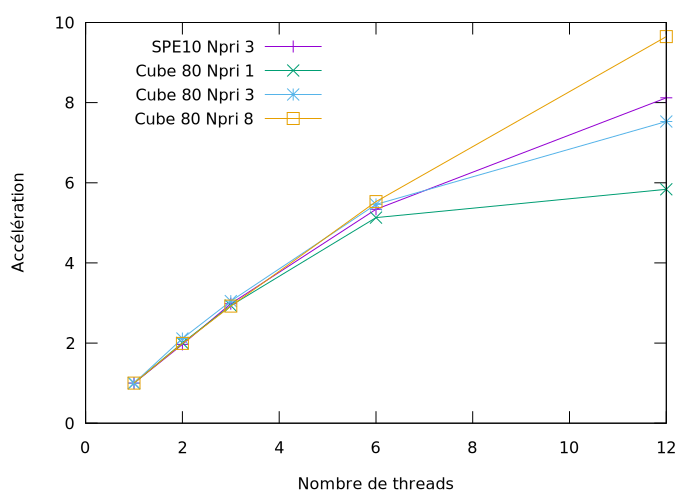
\includegraphics[width=0.7\textwidth]{res_facto_mpi}
  \caption{Performance de la factorisation ILU(0) sur 12 coeurs en utilisant une méthode de Jacobi par blocs.}
  \label{fig:res_facto_mpi}
\end{figure}
%   (-_-)   %
\begin{figure}
  \centering
  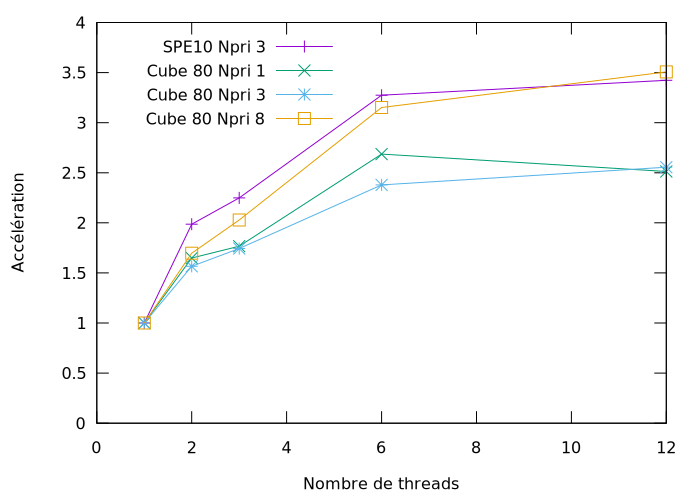
\includegraphics[width=0.7\textwidth]{res_trsv_mpi}
  \caption{Performance de la résolution triangulaire sur 12 coeurs en utilisant une méthode de Jacobi par blocs.}
  \label{fig:res_trsv_mpi}
\end{figure}

Il est nécessaire de regarder du côté de la bande passante mémoire pour trouver des explications.
%
Nous allons maintenant mesurer cette bande passante à l'aide des compteurs matériels.
%
La bande passante utilisée par la méthode Jacobi par blocs est au mieux de 16~Go/s, avec les threads nous utilisons 12~Go/s de bande passante locale dont 5~Go/s de bande passante distante.
%
Cette bande passante distante est le résultat des effets NUMA.
%
Dans le cas des processus MPI utilisée par la méthode Jacobi par blocs, chaque processus a son propre espace mémoire et la localité des données est assurée sous réserve d'un placement statique et optimal des processus.
%
Mais dans le cas des threads, l'espace mémoire est partagé entre deux bancs mémoires et si les accès mémoire ne sont pas optimisés, il y aura des transferts entre les bancs NUMA.
%
Ces transferts auront pour effet d'augmenter la latence des accès mémoire et de réduire le nombre de cycles d'horloge par instruction (CPI\footnote{Clock Per Instruction}), ici on a un CPI de 0,75 pour la version MPI contre 1,08 pour la version threadée.
%
L'explication de la différence de performance entre ces deux versions se situe au niveau de la mémoire, on est limité par la bande passante.
%% +-----------------------------+----------+----------+MPI12
%% |           Metric            |  core 0  |  core 6  |
%% +-----------------------------+----------+----------+
%% |     Runtime (RDTSC) [s]     | 115.248  | 115.248  |
%% |    Runtime unhalted [s]     | 124.295  | 124.907  |
%% |         Clock [MHz]         | 3050.46  | 3053.54  |
%% |             CPI             | 0.751758 | 0.753133 |
%% | Memory bandwidth [MBytes/s] | 15905.1  | 15835.6  |
%% | Memory data volume [GBytes] | 1833.04  | 1825.02  |
%% |  Remote Read BW [MBytes/s]  | 10.3343  | 23.2978  |
%% | Remote Write BW [MBytes/s]  | 0.913861 | 1.61113  |
%% |    Remote BW [MBytes/s]     | 11.2482  | 24.9089  |
%% +-----------------------------+----------+----------+

%% +-----------------------------+----------+----------+MPI6(2*3)
%% |           Metric            |  core 0  |  core 6  |
%% +-----------------------------+----------+----------+
%% |     Runtime (RDTSC) [s]     | 155.807  | 155.807  |
%% |    Runtime unhalted [s]     | 168.391  | 168.976  |
%% |         Clock [MHz]         | 3055.54  | 3055.33  |
%% |             CPI             | 0.544832 | 0.510243 |
%% | Memory bandwidth [MBytes/s] |  11664   | 11561.2  |
%% | Memory data volume [GBytes] | 1817.34  | 1801.31  |
%% |  Remote Read BW [MBytes/s]  | 6.52392  | 31.9625  |
%% | Remote Write BW [MBytes/s]  | 0.532458 | 1.44266  |
%% |    Remote BW [MBytes/s]     | 7.05638  | 33.4051  |
%% +-----------------------------+----------+----------+
%% +-----------------------------+----------+----------+MPI6(1*6)
%% |           Metric            |  core 0  |  core 6  |
%% +-----------------------------+----------+----------+
%% |     Runtime (RDTSC) [s]     | 226.632  | 226.632  |
%% |    Runtime unhalted [s]     | 0.422044 | 245.002  |
%% |         Clock [MHz]         | 2518.14  | 3046.49  |
%% |             CPI             | 1.14334  | 0.728566 |
%% | Memory bandwidth [MBytes/s] | 13.2691  | 16633.6  |
%% | Memory data volume [GBytes] |  3.0072  | 3769.69  |
%% |  Remote Read BW [MBytes/s]  |  5.9309  | 1.91099  |
%% | Remote Write BW [MBytes/s]  | 0.362203 | 0.167456 |
%% |    Remote BW [MBytes/s]     |  6.2931  | 2.07845  |
%% +-----------------------------+----------+----------+

%% +-----------------------------+---------+---------+THREAD_NO_AGG
%% |           Metric            | core 0  | core 6  |
%% +-----------------------------+---------+---------+
%% |     Runtime (RDTSC) [s]     | 1761.37 | 1761.37 |
%% |    Runtime unhalted [s]     | 1679.57 | 1638.75 |
%% |         Clock [MHz]         | 2845.78 | 2792.27 |
%% |             CPI             | 5.57235 | 5.68339 |
%% | Memory bandwidth [MBytes/s] | 5263.52 | 3232.11 |
%% | Memory data volume [GBytes] | 9271.02 | 5692.95 |
%% |  Remote Read BW [MBytes/s]  | 1919.77 | 1341.83 |
%% | Remote Write BW [MBytes/s]  | 170.677 | 112.472 |
%% |    Remote BW [MBytes/s]     | 2090.45 | 1454.3  |
%% +-----------------------------+---------+---------+

%% +-----------------------------+---------+---------+THREAD_AGG_3
%% |           Metric            | core 0  | core 6  |
%% +-----------------------------+---------+---------+
%% |     Runtime (RDTSC) [s]     | 183.336 | 183.336 |
%% |    Runtime unhalted [s]     | 170.046 | 179.213 |
%% |         Clock [MHz]         | 2834.78 | 2872.02 |
%% |             CPI             | 1.08397 | 1.07228 |
%% | Memory bandwidth [MBytes/s] |  11668  |  12351  |
%% | Memory data volume [GBytes] | 2139.16 | 2264.38 |
%% |  Remote Read BW [MBytes/s]  | 5103.69 | 5256.16 |
%% | Remote Write BW [MBytes/s]  | 287.67  | 277.104 |
%% |    Remote BW [MBytes/s]     | 5391.36 | 5533.27 |
%% +-----------------------------+---------+---------+

%-------------------------------
\subsection{Discussion}
Même si un algorithme peut exposer du parallélisme naturellement, il n'est pas toujours possible de l'exploiter correctement.
%
Soit parce qu'il n'y a pas assez de parallélisme pour obtenir un bon équilibrage de charge, soit parce que la granularité du problème n'est pas suffisamment grosse pour négliger les surcoûts liés aux runtimes.
%
Notre proposition permet de manière quasiment transparente d'apporter une solution au problème de la granularité.
%
Mais cette solution n'est pas parfaite, le choix des opérateurs d'agrégation n'est pas automatique et un mauvais choix pourrait être contre performant.
%
Le temps d'application des opérateurs sur le graphe de tâche est aussi un problème, il faut réutiliser le nouveau graphe grossier un certains nombre de fois avant de pouvoir considérer cette étape comme négligeable.
%
Dans le cas où le graphe changerait souvent au cours de l'exécution, cette approche ne fonctionne plus, il faut changer d'algorithme.
%
Une fois les bons opérateurs trouvés, on peut commencer à avoir des résultats proches de l'optimal.
%
C'est le cas pour notre problème mais il reste encore une petite différence à rattraper.
%
Cette différence est due aux effets NUMA, certains accès mémoire auront une latence plus grande que les autres.
%
Il faut donc optimiser le placement des données, le chapitre suivant se concentrera sur l'optimisation des placements mémoires sur machine NUMA.

%+++++++++++++++++++++++++++++++





%=========================================================
\chapter{Limitation de bande passante mémoire}
\minitoc
\vspace{1cm}
%=========================================================

%+++++++++++++++++++++++++++++++
\section{Pourquoi mon SpMV est si lent ?}
%-------------------------------
%+++++++++++++++++++++++++++++++
\section{Pourquoi mon SpMV est si lent ?}
%-------------------------------
\subsection{Deux fois plus de coeurs mais pas deux fois plus rapide}
  \begin{itemize}
    \item Just draw some curves
  \end{itemize}
%-------------------------------
\subsection{Explication de la mémoire}
Pour comprendre les résultats précédent nous devons étudier brièvement l'architecture des ordinateurs.
%
Les performances d'un ordinateur dépendent essentiellement de deux choses : le processeur et la mémoire.
%
Quand un programme souhaite lire une donnée en mémoire, il subit une pénalité mémoire.
%
Cette pénalité est la somme de deux contraintes :
\begin{itemize}
        \item la latence : la différence de temps entre la demande d'accès à la mémoire et la réception du premier octet;
        \item la bande passante : le nombre maximum d'octet par seconde que le bus peut envoyer/recevoir
\end{itemize}
%
In a modern computer, there is different type of memories.
%




  \begin{itemize}
    \item Define memory penalty
    \item Talk about bandwidth
  \end{itemize}
%+++++++++++++++++++++++++++++++

%-------------------------------
\subsection{Explication de la mémoire}
Pour comprendre les résultats précédents nous devons étudier brièvement l'architecture des ordinateurs.
%
Les performances d'un ordinateur dépendent essentiellement de deux choses : le processeur et la mémoire.
%
Quand un programme souhaite lire une donnée en mémoire, il subit une pénalité mémoire.
%
Cette pénalité est la somme de deux contraintes :
\begin{itemize}
        \item la latence : la différence de temps entre la demande d'accès à la mémoire et la réception du premier octet;
        \item la bande passante : le nombre maximum d'octet par seconde que le bus peut envoyer/recevoir
\end{itemize}
%
De nos jours, les ordinateurs ont différents types de mémoires.
%
Il y a la mémoire cache, très proche des unités de calcul, elle a une faible latence (quelques cycles) mais sa taille est limité à quelques Mo.
%
Ensuite, il y a la mémoire RAM avec une latence de quelques centaines de cycles mais avec une taille de plusieurs Go.
%
Si nous regardons la structure mémoire de deux bancs NUMA de la figure~\ref{fig:numa_architecture}, on s'aperçoit que la distance physique des coeurs de calcul et de la mémoire est liée à la latence des accès mémoires.
%
Pour obtenir limiter le plus possible les pénalités mémoires, il est nécessaire que tous les coeurs de calcul utilisent la mémoire qui est la plus proche.
%
Si un coeur du banc NUMA gauche doit accéder à la mémoire du banc NUMA droit, il aura une plus grande pénalité mémoire que

%   (-_-)   %
\begin{figure}[t!]
  \centering
  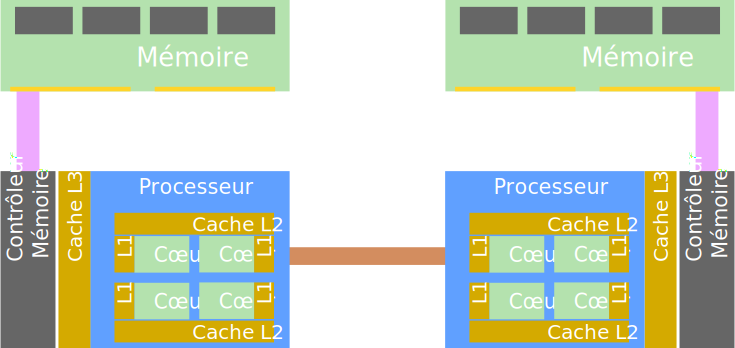
\includegraphics[width=0.8\textwidth]{numa_architecture}
  \caption{Exemple d'une architecture NUMA à deux processeurs.}
  \label{fig:numa_architecture}
\end{figure}

Un autre problème se situe au niveau de la bande passante.
%
La bande passante totale de la machine est distribuée entre chaque banc NUMA.
%
Pour exploiter efficacement la totalité de la bande passante, il faut répartir les données que l'on va utiliser sur tous les bancs mémoires.
%
Il ne suffit pas de faire une répartition équitable, il faut aussi au moment de l'accès au données que tous les coeurs de calcul accède à des données différentes qui doivent se situer dans la mémoire qui leurs est la plus proche.

%+++++++++++++++++++++++++++++++


%+++++++++++++++++++++++++++++++
\section{Gestion actuelle des machines NUMA}
De manière générale, quand un programme alloue de la mémoire, il reçoit un pointeur sur de la mémoire virtuelle.
%
Cette mémoire virtuelle est unique à chaque processus et est partagée entre les threads.
%
La relation entre la mémoire virtuelle et la mémoire physique est faite par le système d'exploitation.
%
Il est en charge de la bonne gestion de la mémoire physique.
%
Lorsqu'un processus accède à de la mémoire virtuelle qui n'as pas encore été mappée à de la mémoire physique, une faute de page est générée, on appelle ça toucher une page.
%
Cette faute est traitée par le système d'exploitation, il s'occupera de trouver une page mémoire libre dans la mémoire physique et il la fera correspondre à une adresse virtuelle.
%
Lors des accès mémoire du processus, la traduction de l'adresse virtuelle vers l'adresse physique est faite par un des composant du processeur, l'unité de gestion mémoire ou MMU\footnote{Memory Management Unit}.
%
De cette façon, le processus ne voit que l'espace d'adressage virtuelle et ne connaît rien de l'espace d'adressage physique.
%
Le système d'exploitation peut donc changer l'emplacement physique d'une page sans affecter le fonctionnement du processus, c'est totalement transparent.
%
Toutefois, l'emplacement physique d'une page virtuelle peut impacter les performances du processus sur les architectures NUMA.
%
Cet impact dépendra des connexions entre le banc mémoire physique où se situe la page et le coeur de calcul qui fait tourner le processus.


Sur une machine NUMA, lorsqu'une faute de page arrive, le système d'exploitation doit choisir sur quel banc NUMA il placera la page.
%
Avec Linux, il y a au moins trois politiques d'allocations de disponibles :
\begin{itemize}
        \item {\em First Touch}: La mémoire est allouée sur le banc NUMA du coeur de calcul qui y accède en premier.
                         Il s'agit de la politique par défaut.
        \item {\em Bind}: La mémoire est allouée sur banc NUMA spécifié en paramètre.
        \item {\em Interleaved}: Les allocations mémoire sont entrelacées parmi tous les bancs NUMA disponibles.
\end{itemize}
Sur Linux, ces politiques peuvent être choisies avec l'appel système {\em mbind}, ou avec l'outil en ligne de commande {\em numactl}.
%
La version 3.13 de Linux apporte un nouveau mécanisme de gestion de la mémoire sur les machines NUMA, il s'agit d'AutoNUMA.
%
Ce mécanisme a pour but d'optimiser le placement des pages NUMA tout long de l'exécution d'un processus (Voir section~\ref{sec:autonuma}).


D'autres systèmes d'exploitation peuvent avoir leurs propres ensembles de politiques d'allocations NUMA.
%
Solaris, par exemple, fournit aussi la politique {\em next-touch}~\cite{next_touch}.
%
Avec cette politique, les pages mémoires physique seront déplacées près du prochain coeur de calcul qui y accédera (Voir section~\ref{sec:next_touch}).

%-------------------------------
\subsection{First touch}
La politique d'allocation mémoire par défaut sous Linux s'appelle {\em First Touch}.
%
La traduction littérale serait le {\em premier toucher}, ce nom se réfère au fait qu'avec cette allocation le noyau associe une nouvelle page physique à une page virtuelle qu'à partir de la première utilisation de cette page.
%
La page physique sera choisie avec comme priorité de prendre une page dans la mémoire la plus proche du thread qui souhaite utiliser cette page.
%
L'idée derrière cette allocation n'est pas mauvaise, dans le cas d'un processus mono-thread dont l'affinité processeur est fixée à un banc mémoire, la localité mémoire sera toujours optimale.
%
Dans le cas d'un processus multi-threads dont les threads ont une affinité fixe, s'ils allouent eux-mêmes leurs mémoires et ne font presque aucun partage entre eux, cette allocation fonctionne toujours.
%
Mais tous les programmes ne sont pas écrits pour fonctionner de cette façon.
%
Imaginons un programme qui soit écrit pour avoir une phase d'initialisation séquentielle, avec toutes les allocations dont il aura besoin dans cette phase, alors toute la mémoire physique sera allouée sur un seul banc NUMA.
%
Comme toutes les données se retrouvent exclusivement sur un seul banc NUMA, tous les threads devront se partager la bande passante mémoire de ce banc alors que les bandes passantes des autres bancs NUMA seront utilisées.


Il existe d'autres cas où ce type d'allocation ne permet pas d'obtenir le maximum de bande passante mémoire de la machine.
%
Par exemple dans le cas d'une application multi-processus dont tous les processus ont une affinité processeur identique et fixée à un seul banc NUMA.
%
Seulement une partie de la bande passante mémoire sera utilisée.
%
Il y a aussi le cas où les processus ont une affinité processeur leurs permettant d'utiliser n'importe quel coeur de la machine.
%
L'allocation des pages mémoires peut se faire sur un banc NUMA, puis le noyau décide de changer le processus de banc NUMA, et tous les calculs sont faits avec une mauvaise localité mémoire.
%
De plus, si le thread de calcul change souvent de coeur de calcul, l'utilisation des caches de faibles niveaux (L1 et L2) ne sera pas optimale.
%
Il est donc important de toujours fixer l'affinité processeur d'un thread à un coeur de calcul.
%
Dans notre programme, l'initialisation des données est séquentielle. Donc avec une politique d'allocation first touch, toutes les données se retrouvent sur un seul banc NUMA.
%
Nous avons donc plusieurs choix pour distribuer les données :
\begin{itemize}
  \item soit nous réécrivons la partie initialisation pour qu'elle soit faite en parallèle;
  \item soit nous essayons une autre politique d'allocation qui correspond mieux à notre problème.
\end{itemize}
%
La première solution est compliquée à mettre en oeuvre et pourrait introduire de nouveaux bogues dans le code.
%
La deuxième solution nécessite moins de changement, nous avons donc essayé cette solution.

%-------------------------------
\subsection{Interleaved memory}
First touch n'étant pas parfait, il est nécessaire d'avoir d'autres politiques d'allocation.
%
La politique {\em Interleaved memory} distribue uniformément les pages mémoires sur tous les bancs mémoires en mode tourniquet.
%
Cette distribution est faite par le noyau du système d'exploitation au moment où une page mémoire est utilisée pour la première fois par le programme.
%
Sur un système d'exploitation utilisant Linux comme noyau, il suffit d'utiliser la commande {\em numactl --interleave=all ./programme} pour utiliser cette politique d'allocation dans tout le programme.
%
En plus d'avoir très peu d'impact sur le code source d'une application, la politique d'entrelacement mémoire montre des atténuations des effets NUMA dans le cas général.
%
En moyenne, il n'y a pas d'amélioration de la latence, mais la bande passante est améliorée grâce à l'utilisation simultanée de tous les liens mémoires par rapport à une initialisation séquentielle avec une politique first touch.
%
Ainsi, il est généralement intéressant d'expérimenter cette politique, avant d'étudier la question des optimisations NUMA.
%
Dans notre cas, cette politique nous donnait de meilleurs performances que la politique first touch.
%
Mais les résultats n'étaient pas suffisant.

%-------------------------------
\subsection{Next touch}
\label{sec:next_touch}
L'idée du First touch n'est pas mauvaise, mais elle impose une phase d'initialisation parallèle.
%
Au lieu de récrire toute l'initialisation d'un programme, il pourrait être intéressant d'utiliser les phases de calculs pour distribuer la mémoire sur tous les bancs NUMA.
%
C'est pour cela que la politique d'allocation {\em next touch} a été créée.
%
Le programmeur choisit un ensemble de pages mémoires qu'il pense mal placées et définit une politique d'allocation next touch sur ces pages.
%
Lors du prochain accès mémoire à l'une de ces pages, le noyau s'occupera, si besoin, de déplacer la page mémoire vers le banc NUMA le plus proche du processeur faisant cet accès.
%
Ainsi nous pouvons obtenir une amélioration de la localité mémoire sans avoir à récrire certaines parties du code.
%
Cette politique aurait pu apporter des performances supplémentaires à notre code, mais n'étant pas disponible dans le noyau Linux, malgré des propositions d'extensions~\cite{next_touch_linux,GoFu09Next-touch}, nous n'avons pas pu l'utiliser telle quelle.
%
\`A la place, nous avons implémenté une solution similaire qui consiste à choisir manuellement l'emplacement des pages mémoires.

%-------------------------------
\subsection{AutoNUMA}
\label{sec:autonuma}
Linux n'a pas adopté la politique d'allocation Next touch.
%
\`A la place, les développeurs de Linux ont choisi d'implémenter un autre mécanisme pour améliorer la localité NUMA : {\em AutoNUMA}.
%
Ce mécanisme va scanner périodiquement une portion de la mémoire d'un processus, et de la même façon que la politique next touch, le prochain accès à une page de cette portion entraînera un déplacement de la page.
%
Pour détecter l'accès à une page, le noyau utilise la MMU.
%
Il supprime la relation adresse virtuelle vers adresse physique de la MMU et peut ainsi recevoir un signal lors du prochain accès.
%
Ce mécanisme à un surcoût, c'est pourquoi il n'est pas appliqué sur toute la mémoire d'un coup.
%
Le noyau donne la possibilité de modifier plusieurs paramètres de ce mécanisme, mais ces paramètres sont globaux.
%
Parmi ces paramètres, il y a {\em scan\_delay} et {\em scan\_size}.
%
Tous les ``scan\_delay'', les ``scan\_size'' pages suivantes sont traitées.
%
Une fois arrivé au bout de l'espace d'adressage, le scanner recommence au début de l'espace d'adressage.
%
La variable scan\_delay change de valeur en fonction du nombre de pages déplacées.
%
Elle diminue quand il y a beaucoup de fautes NUMA et augmente quand les pages sont bien placées.
%
Ainsi, une application dont les threads accèdent toujours à la même mémoire aura automatiquement un bon placement mémoire.


Ce mécanisme comporte plusieurs défauts.
%
Sa configuration est globale au système, on ne peut pas l'activer que pour un processus particulier.
%
Les paramètres ne peuvent être définis que par l'administrateur de la machine.
%
Le mécanisme s'applique sur toute la mémoire, même les zones mémoires peu utilisées.

%-------------------------------
\subsection{Un processus MPI par banc NUMA}
Les problèmes rencontrés sur les machines NUMA proviennent essentiellement de la mémoire partagée.
%
Lorsque deux threads partagent un espace mémoire et que ces deux threads s'exécutent sur des bancs NUMA différents, il y aura potentiellement des accès mémoire non performants.
%
Nous pouvons donc résoudre le problème des effets NUMA en utilisant plusieurs processus.
%
En utilisant un processus MPI par banc NUMA et une politique d'allocation first touch ou bind, on se retrouve toujours avec des accès mémoire sur le banc mémoire le plus proche.
%
Mais la problématique reste similaire à la problématique du choix entre la parallélisation en mémoire distribuée et la parallélisation en mémoire partagée, ce n'est pas toujours possible ou performant.
%
Dans le cas où les algorithmes en mémoire distribuée ne passeraient pas à l'échelle, il est nécessaire de noter que l'utilisation de cette solution multipliera le nombre de processus MPI par le nombre de bancs NUMA.
%
Notre application utilise déjà du parallélisme en mémoire distribuée, il n'y aura donc pas de modification à effectuer pour cette solution.
%
Par contre, les algorithmes que nous utilisons donnent de meilleurs résultats avec peu de processus MPI, nous cherchons donc à limiter le nombre de processus MPI.

%+++++++++++++++++++++++++++++++



%+++++++++++++++++++++++++++++++
\section{Gérer le NUMA directement dans l'ordonnanceur}
%-------------------------------
\subsection{Statuts des ordonnanceurs actuels}
La gestion du placement des pages mémoires n'est pas utile si le code qui utilisera ces données ne s'exécute pas sur un coeur associé au bon banc NUMA.
%
Dans le cas de la programmation par tâche, chaque tâche doit connaître le banc NUMA qui lui est le plus favorable.
%
Cette information pourra être ensuite donnée à l'ordonnanceur de tâches qui s'occupera de placer correctement la tâche.


ForestGOMP\cite{Bro10Thesis} est le résultat d'un travail de recherche autour du support des machines à mémoires hiérarchiques dans OpenMP.
%
Il utilise le parallélisme de boucle imbriqué pour adresser les différents niveaux hiérarchiques de la machine.
%
La bibliothèque de threads Marcel\cite{marcel} est utilisée pour la création de thread en espace utilisateur.
%
Dans une première boucle for sur le nombre de noeuds NUMA, le programmeur déclare les données auxquelles il va accéder.
%
Dans une deuxième boucle for imbriquée, le programmeur effectue les calculs.
%
L'utilisation de threads en espace utilisateur permet de créer un grand nombre de threads sans trop impacter la performance.
%
En créant un nombre conséquent de threads, nous pouvons obtenir un bon équilibrage de charge.
%
Cet équilibrage de charge sera possible grâce à l'utilisation de BubbleSched\cite{bubblesched} qui permet de créer des bulles de threads pour pouvoir déplacer un ensemble de threads sur un nouveau coeur de calcul d'un coup.
%
Lorsque le travail vient à manquer, c'est-à-dire qu'il n'y a plus assez de bulles pour occuper tous les coeurs de calcul, on peut exploser une bulle qui se transformera en plusieurs bulles jusqu'à atteindre la granularité d'un thread.
%
Les informations mémoires étant associées aux bulles, il est possible de choisir la meilleure bulle à éclater, celle qui nous fournira les meilleurs accès mémoire.
%
La gestion des allocations mémoires de ForestGOMP repose sur MaMI\footnote{Marcel Memory Allocator}, une bibliothèque écrite spécialement pour exploiter les machines NUMA dans Marcel.
%
MaMI implémente la politique d'allocation next touch et permet aussi la migration explicite des données.
%
ForestGOMP se base donc sur le principe que le programmeur est le mieux placé pour connaître l'utilisation mémoire de son programme.
%
Ces travaux montrent qu'une meilleure gestion des allocations mémoires, même manuelle, permet de gagner en performance.


PaRSEC est un cadriciel de parallélisation par tâche qui fonctionne aussi en mémoire distribuée.
%
Il est l'un des seuls ordonnanceurs de tâches à offrir un réel support des architectures NUMA.
%
Par contre son support est une analogie avec la programmation en mémoire distribuée.
%
En effet, le support du NUMA est fait avec les structures Virtual Process (VP) de PaRSEC, ce qui peut correspondre à avoir un processus MPI par banc NUMA.
%
Mais ce n'est pas si grave, le vol de tâche entre VP existe.
%
Il conserve donc l'aspect équilibrage de charge des solutions multithreadées.
%
Par contre, cette solution ne convient toujours pas à résoudre notre problème, nous essayons d'avoir le moins possible de parallélisme en mémoire distribuée.

MAi\footnote{Memory Affinity Interface}\cite{mai} fournit une interface de placement des données.
%
Par rapport à MaMI, MAi implémente des stratégies génériques d'allocations des pages mémoires.
%
Mais MAi ne fournit pas d'ordonnanceur de tâches, nous ne pourrons donc pas exécuter les tâches sur les noeuds de calcul où la mémoire est allouée.


D'autres tentatives d'extension de la spécification OpenMP existent.
%
L'article~\cite{openmp_numa} présente l'ajout de trois nouvelles directives pour OpenMP.
%
La première directive se concentre sur la migration des données lors du prochain accès à ces données, il s'agît d'une implémentation de la politique d'allocation next touch.
%
La deuxième directive concerne la distribution des pages d'une zone mémoire.
%
Cette distribution peut être faite par bloc, entrelacé sur différents bancs NUMA dans plusieurs dimensions.
%
La troisième directive permet de prévenir l'ordonnanceur que la distribution des itérations d'une boucle doit tenir compte des allocations NUMA.
%
Les performances obtenues sur une factorisation LU dense sont encourageantes, une accélération quasi parfaite jusqu'à 16 processeurs là où une version OpenMP classique est deux fois moins performante.
%
Ces travaux nous prouvent qu'une gestion fine des allocations NUMA couplée à un ordonnanceur prenant en compte les affinités mémoires permet d'exploiter efficacement une machine NUMA.
%
Malheureusement, seul le parallélisme de boucle est traité, il n'y a pas gestion du parallélisme à base de graphe de tâches.


Des runtimes comme StarPU ou OmpSs demandent au programmeur de décrire les données utilisées par les tâches de calcul.
%
Cette information est ensuite utilisée pour effectuer des transferts vers d'autres types de mémoires.
%
Il est regrettable qu'aucun de ces runtimes n'utilise cette information pour optimiser les accès mémoire sur des machines NUMA.

%-------------------------------
\subsection{NATaS : ordonnancer des tâches sur une machine NUMA}
Aucune des solutions proposées dans la section précédente ne correspondait à notre besoin, nous avons créé notre propre ordonnanceur de tâches.
%
Nous l'avons appelé NATaS, il s'agit de l'acronyme {\em Numa Aware Task Scheduler}.
%
Celui-ci est très basique, il ne prend en compte que l'affinité mémoire des tâches, la gestion des dépendances est laissée à Taggre, tout comme avec les ordonnanceurs OpenMP et TBB.
%
Pour ordonnancer les tâches avec la meilleure affinité mémoire possible, nous utilisons un conteneur de tâches thread-safe par banc NUMA.
%
Ce container permet à plusieurs threads d'insérer/retirer des tâches en limitant la contention.
%
Le vol de tâche entre conteneurs a aussi été implémenté, il existe une option par tâche pour autoriser ou non le vol de tâche.
%
Dans le cas du parallélisme de boucle, une option permettant de donner une tâche spécifiquement à un thread a été implémentée.

Contrairement à la plupart des autres ordonnanceurs de tâches, nous n'utilisons pas un conteneur de tâches par thread, mais un conteneur par banc NUMA.
%
Nous avons donc plus de contention sur cette structure et une queue basique ne serait pas assez efficace.
%
\`A la place, nous utilisons un conteneur sans verrou, entièrement construit autour de l'instruction compare-and-swap.
%
Nous limitons donc les processeurs capables de faire fonctionner NATaS à ceux ayant l'instruction compare-and-swap.
%
Cette structure ne nous permet pas d'obtenir les mêmes performances que l'utilisation d'une queue par thread, mais elle a l'avantage de mieux fonctionner pour l'équilibrage de charge à l'intérieur d'un banc NUMA.



NATaS fournit aussi une API permettant de gérer les allocations mémoires et leurs placements.
%
Il permet de faire différents types d'allocations tels que :
\begin{itemize}
  \item distribuer régulièrement la mémoire en mode bloc;
  \item entrelacer les pages mémoires;
  \item spécifier l'emplacement mémoire.
\end{itemize}
%
Ces allocations font miroir aux différentes politiques de gestion mémoires (first touch, interleave et bind).
%
Dans le cas d'un parallélisme de boucle avec une distribution statique, on distribuera la mémoire régulièrement.
%
Cet espace mémoire sera découpé en autant de blocs qu'il y a de bancs NUMA sur la machine.
%
Puis chaque bloc sera placé sur un banc NUMA.


Taggre utilisera l'interface de NATaS pour améliorer les performances sur des machines NUMA.
%
Il fournira au programmeur une interface simplifié permettant de déplacer la mémoire juste en déclarant pour chaque tâche la mémoire utilisée dans celle-ci.
%
La connaissance complète du graphe de tâches permet des améliorations notables sur la distribution mémoire.
%
Dans un premier temps, on va équilibrer la distribution des tâches sur les bancs NUMA en attribuant une affinité NUMA aux tâches (Fig.~\ref{fig:numa_distrib_example}).
%
Comme le graphe sera déroulé de haut en bas lors de son exécution, il parait naturel de distribuer les tâches par hauteur.
%
En supposant que les tâches produisent des données et que ces données sont passées en paramètre aux tâches successeurs dans le graphe, on peut essayer d'optimiser le placement NUMA.
%
Cette affinité sera choisie en fonction de la hauteur de la tâche dans le graphe et des affinités NUMA de ses prédécesseurs.
%
Le but étant d'avoir à hauteur fixée, un nombre égale de tâche par banc NUMA tout en minimisant les accès en lecture distante.
%
Une fois l'affinité NUMA de toutes les tâches définies, il ne nous reste plus qu'à connaître les données utilisées.
%
Donc dans un deuxième temps, le programmeur indiquera les données utilisées dans chaque tâche.
%
Pour cela, il lui suffira de simuler l'exécution du code, de désactiver le vol de tâches et d'appeler la fonction d'enregistrement mémoire.
%
Nous obtiendrons ainsi une mémoire équitablement distribuée et des accès mémoire optimisés.


\lstinputlisting[inputencoding=utf8/latin1,caption=Exemple de code permettant d\'eplacer la m\'emoire sur une machine NUMA avec Taggre,frame=single,float=t]{src/natas.cpp}


%   (-_-)   %
\begin{figure}[!h]
  \centering
  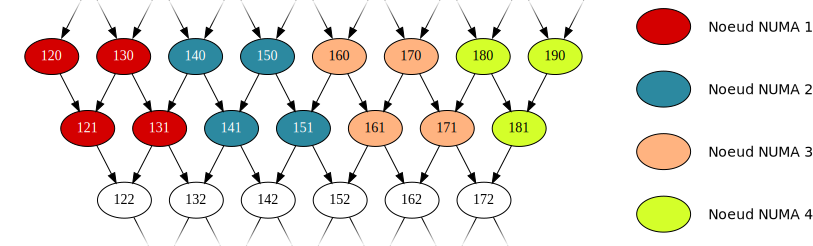
\includegraphics[width=\textwidth]{numa_distrib_example}
  \caption{Exemple de l'algorithme de distribution des tâches en action, la couleur des tâches détermine leurs affinités NUMA. Les tâches en blanches ne sont pas encore traitées.}
  \label{fig:numa_distrib_example}
\end{figure}

%+++++++++++++++++++++++++++++++


%+++++++++++++++++++++++++++++++
\section{Results}
%-------------------------------
\subsection{Factorization and Triangular solve}
  \begin{itemize}
    \item Support NUMA in tasks
  \end{itemize}
%-------------------------------
\subsection{Multiplication matrice vecteur creuse}
La multiplication du matrice creuse par un vecteur est une opération dont le ratio nombre d'opérations par le nombre d'octet lus est petit.
%
Dans le cas d'une matrice scalaire, ce ratio vaut environ $1/10$ en double précision.
%
Pour chaque valeur non-nulles de la matrice, il faut lire cette valeur, l'indice de la colonne et la valeur contenue dans le vecteur à l'indice de la colonne.
%
Il faut ensuite multiplier les deux valeurs ensemble et l'ajouter à un accumulateur, ce qui fait en double précision 2 opérations pour 20 octets lus.
%
Si nous utilisons trois variables primaires, chaque entrée de la matrice est un bloc 3 par 3.
%
Nous devons donc lire ce bloc (9*8 Octets), lire l'indice de colonne (4 Octets) et finalement lire 3 valeurs dans le vecteur (3*8 Octets).
%
Pour chaque valeur du bloc nous avons 2 opérations à faire (2*9), nous avons donc un ratio de $18/100$ soit environ $1/5,5$.
%
Avec huit variables primaires, le ratio monte à environ de $1/4,5$.


Le {\em roofline model} est un modèle de performance permettant de connaître la puissance de calcul maximale pouvant être atteinte par un algorithme sur une machine.
%
Ce modèle se construit de la façon suivante, dans un premier temps nous allons mesurer la bande passante maximale de la machine.
%
Pour cela nous avons utilisé le benchmark STREAM, sur Rostand, nous obtenons une bande passante de 21~Go/s.
%
Puis, dans un second temps, nous allons calculer la capacité de calcul maximale de la machine.
%
Pour calculer cette capacité, il faut multiplier le nombre de coeur de calcul par le nombre maximal d'opérations faites dans une instruction et multiplier le tout pas la fréquence d'horloge.
%
Chaque noeud de Rostand étant composé de 12 coeurs cadencés à 2,80~GHz et du jeu d'instructions SSE~4.2 permettant d'effectuer 4 opérations flottantes en simple précision à la fois, ce qui donne 134,4~GFlops.
%
Le nombre d'opérations simultanées en double précision est divisé par 2, donc on peux avoir au maximum 67,2~GFlops et si nous n'utilisons pas le jeu d'instructions vectorielles, nous pouvons obtenir au maximum 33,6~GFlops (Fig.~\ref{fig:roofline_rostand}).


Une fois le roofline model construit, nous pouvons donc placer le produit matrice vecteur creux.
%
Les performances du SpMV dépendent du nombre de variables primaires, nous avons donc placé sur le roofline model trois SpMV en fonction du nombre de variable primaire utilisées.
%
Ces trois points nous indiquent que les performances du SpMV seront limitées par la bande passante mémoire.
%
L'utilisation du jeu d'instructions vectorielles aura donc très peu d'impact sur nos performances.
%
Nous devons nous concentrer sur les accès mémoires et surtout dans notre cas, sur les effets NUMA.

%   (-_-)   %
\begin{figure}
  \centering
  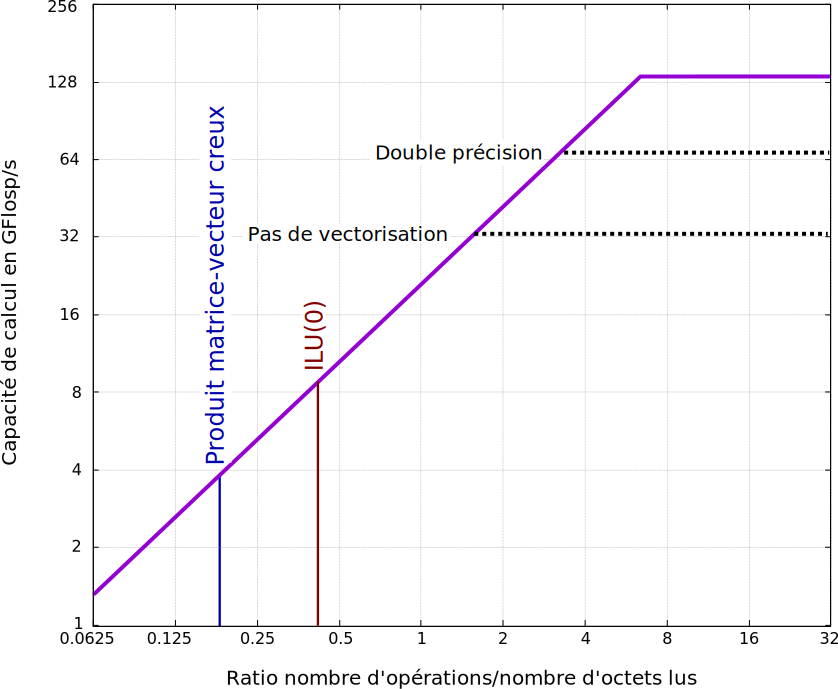
\includegraphics[width=0.8\textwidth]{roofline_rostand}
  \caption{Roofline model de Rostand avec les différents produit matrice vecteur creux.}
  \label{fig:roofline_rostand}
\end{figure}


% -------------------------------
\subsubsection{Mémoire distribuée}
Le produit matrice vecteur creux, que j'abrégerai SpMV pour le reste des résultats, est un algorithme qui se parallélise très bien en mémoire partagée.
%
Nous pouvons donc estimer que la performance atteinte en mémoire distribuée est une borne maximale à atteindre en mémoire partagée.
%
En effet, de par sa nature distribuée, les pénalités mémoires NUMA sont minimales.
%
Le roofline model prédit un algorithme limité en performance par la bande passante mémoire.
%
Or, cette bande passante mémoire est partagée entre les coeurs d'un même banc NUMA.
%
L'accélération obtenue sera donc limité par la bande passante mémoire.
%
Sur la machine rostand, la bande passante mémoire limite grandement cette accélération (fig.~\ref{fig:res_spmv_mpi_rostand}).
%
Avec un cas à 8 variables primaires, nous obtenons une accélération maximal de 3,8.
%
La capacité de calcul mesuré avec 12 coeurs est de 4,96~GFlops, cela correspond à la prédiction du roofline model.


%   (-_-)   %
\begin{figure}[t!]
  \centering
  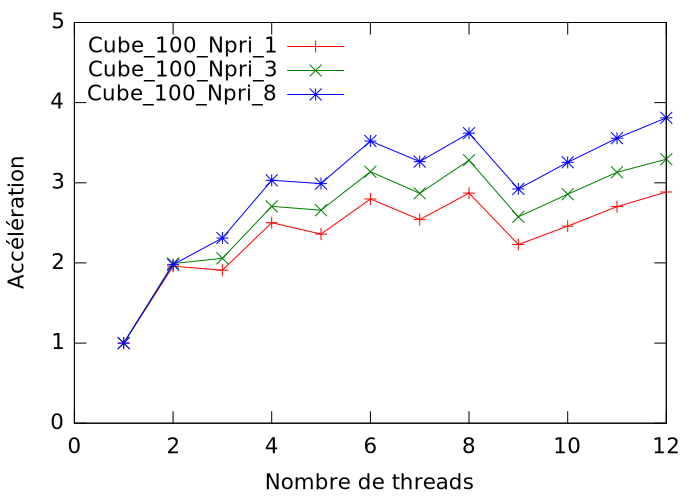
\includegraphics[width=0.7\textwidth]{res_spmv_mpi}
  \caption{Accélération du produit matrice vecteur creux sur Rostand en mémoire distribuée.}
  \label{fig:res_spmv_mpi_rostand}
\end{figure}



Sur Manumanu, nous avons beaucoup plus de banc NUMA, ce qui signifie que nous aurons plus de bande passante mémoire à notre disposition.
%
Nous pouvons donc espérer avoir de meilleurs résultats que sur Rostand.
%
Il faut aussi prendre en compte une bande passante mémoire plus élevée sur les banc NUMA de Manumanu que sur ceux de Rostand.
%
Les processus MPI sont alloués en mode compact, c'est à dire qu'ils sont distribués de façon à utiliser un minimum de noeuds NUMA.
%
Sur 1 banc NUMA, nous avons une accélération de 5 avec 8 variables primaires (fig~\ref{fig:res_spmv_mpi_manu}).
%
Cette accélération monte à 110 avec l'utilisation des 20 bancs NUMA et des 160 coeurs.


%   (-_-)   %
\begin{figure}[t!]
  \centering
  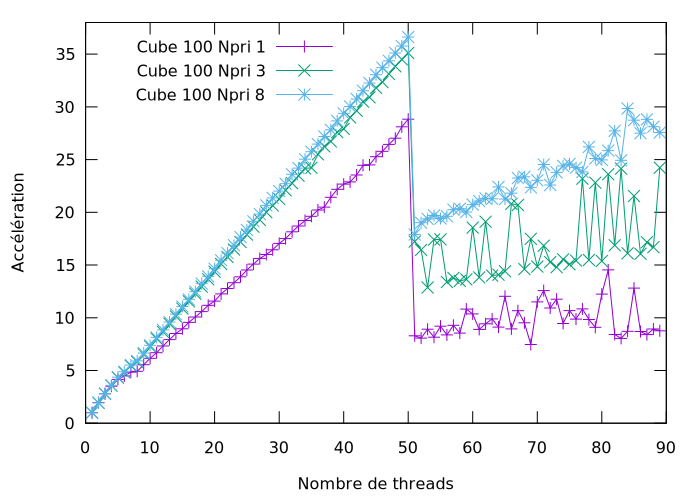
\includegraphics[width=0.7\textwidth]{res_spmv_mpi_manu}
  \caption{Accélération du produit matrice vecteur creux sur Manumanu en mémoire distribuée.}
  \label{fig:res_spmv_mpi_manumanu}
\end{figure}

% -------------------------------
\subsubsection{First touch}
Nous allons maintenant nous concentrer sur la parallélisation du SpMV en mémoire partagée.
%
La mémoire est allouée sur un seul banc NUMA et le travail est partagée par une directive {\em \#pragma omp parallel for}.
%
Sur la machine Rostand, nous obtenons difficilement une accélération de 2,5 sur 12 coeurs en ayant 8 variables primaires (Fig.~\ref{fig:res_spmv_ft_rostand}).
%
Cette accélération descend à 1,9 en ayant 1 variable primaire, toujours sur 12 coeurs de calcul.
%
Ces résultats sont à comparer avec ceux obtenues en mémoire distribuée.
%
Nous n'obtenons que 65~\% de la puissance maximale que nous devrions avoir.
%
Le SpMV étant limité par la bande passante mémoire, l'utilisation d'un seul banc NUMA pour les accès mémoire ne nous permet pas d'exploiter toute la puissance de la machine.




Sur la machine Manumanu, ces effets sont amplifiés (Fig.~\ref{fig:res_spmv_ft_manu}).
%
Nous obtenons les meilleures performances en utilisant 8 coeurs avec une accélération de 5-6.
%
Utiliser plus de 8 coeurs pour effectuer le SpMV fait perdre du temps, les données étant toute sur le premier banc NUMA, nous utilisons uniquement la bande passante de ce banc avec des latences d'accès plus ou moins longues.
%
Les résultats en mémoire distribuée sont meilleurs.
%
Pour obtenir les mêmes performances qu'en mémoire distribuée, nous devons optimiser les accès mémoire.

% -------------------------------
\subsubsection{Interleave}
Pour diminuer les effets NUMA, nous pouvons utiliser la politique d'allocation interleave.
%
Cette politique va distribuer uniformément les pages mémoires sur les différents bancs NUMA.
%
Nous allons donc augmenter la bande passante mémoire en ne modifiant que la latence mémoire moyenne.
%
Sur Rostand, nous obtenons un gain de performance d'environ 20~\% mais les performances sont toujours en dessous des performances obtenues en mémoire partagée (Fig.~\ref{fig:res_spmv_interleave_rostand}).

%   (-_-)   %
\begin{figure}[t!]
  \centering
  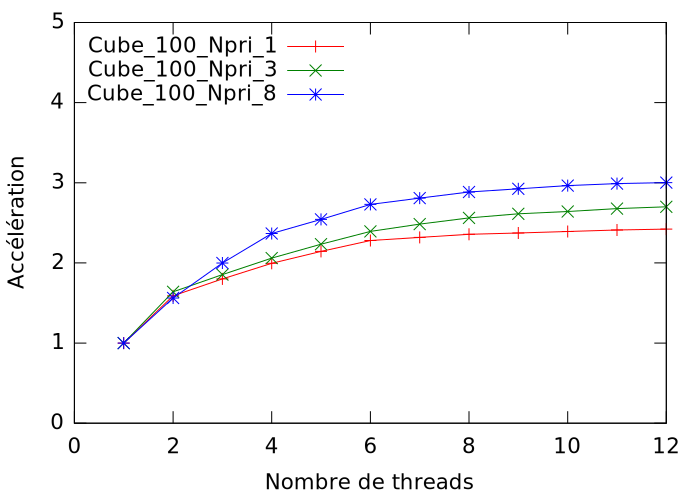
\includegraphics[width=0.7\textwidth]{res_spmv_interleave}
  \caption{Accélération du produit matrice vecteur creux sur Rostand en mémoire partagée avec une politique d'allocation interleave.}
  \label{fig:res_spmv_interleave_rostand}
\end{figure}

Sur Manumanu, on obtient de bons résultats jusqu'à 16 coeurs (Fig.~\ref{fig:res_spmv_interleave_manumanu}).
%
Au delà, nous commençons à utiliser le SGI$^\registered$ NUMAlink$^{\rm TM}$\cite{numalink} et les temps de latence des accès mémoire augmentent.
%
En effet, la majorité des accès mémoire se font sur des bancs NUMA distant.
%
Au final, les résultats de l'allocation interleave sur Manumanu sont proches des résultats de l'allocation first touch.
%
Ce n'est donc pas la bonne solution pour exploiter les performances de cette machine.

%   (-_-)   %
\begin{figure}[t!]
  \centering
  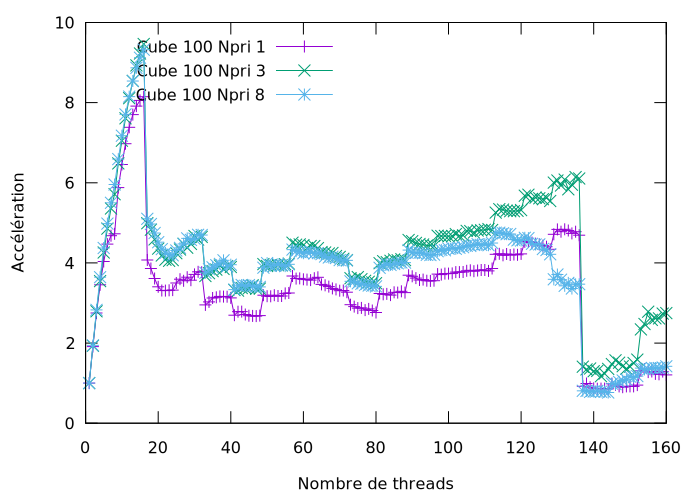
\includegraphics[width=0.7\textwidth]{res_spmv_interleave_manu}
  \caption{Accélération du produit matrice vecteur creux sur Manumanu en mémoire partagée avec une politique d'allocation interleave.}
  \label{fig:res_spmv_interleave_manumanu}
\end{figure}

%-------------------------------
\subsection{NATaS}
\`A la différence des autres ordonnanceurs, NATaS va tenir compte de l'affinité NUMA des tâches.
%
Cette affinité a été définit par Taggre de tel sorte à équilibrer la charge sur les différents banc NUMA.
%



Sur plusieurs bancs NUMA, NATaS offre des meilleurs performances que l'ordonnanceur OpenMP même avec l'allocation mémoire interleaved.
%
{\em Donner résultat manumanu}
%

%-------------------------------
\subsubsection{\'Equilibrage automatique NUMA}
Les noyaux Linux récents proposent un équilibrage de charge automatique des pages mémoires.
%
Malheureusement, nous ne pouvons pas utiliser les grappes de serveurs à notre disposition pour tester cette fonctionnalité.
%
La version de Linux disponible sur ces machines n'est pas assez récente, la fonctionnalité AutoNUMA n'est apparue que dans la version 3.13 du noyau.
%
\`A la place, nous allons utiliser une machine de bureau contenant deux processeurs Intel Xeon X5660, chaque banc NUMA dispose de 6 coeurs de calculs et de 24~Go de mémoire vive.
%
La version de Linux utilisée est la 3.18.

Cette méthode ne fonctionne que lorsque le programme est exécuté suffisamment longtemps pour avoir le temps d'analyser toute la mémoire utilisée.
%
Nous allons chercher l'accélération maximale que nous pouvons atteindre avec cette solution.
%
Il ne nous est donc pas utile de faire varier le nombre de coeurs de calcul, nous utiliserons les 12 coeurs de calcul de la machine.
%
Nous allons plutôt faire varier le nombre de SpMV pour faire varier le temps d'exécution du programme et laisser au noyau assez de temps pour déplacer les pages.

%   (-_-)   %
\begin{figure}
  \centering
  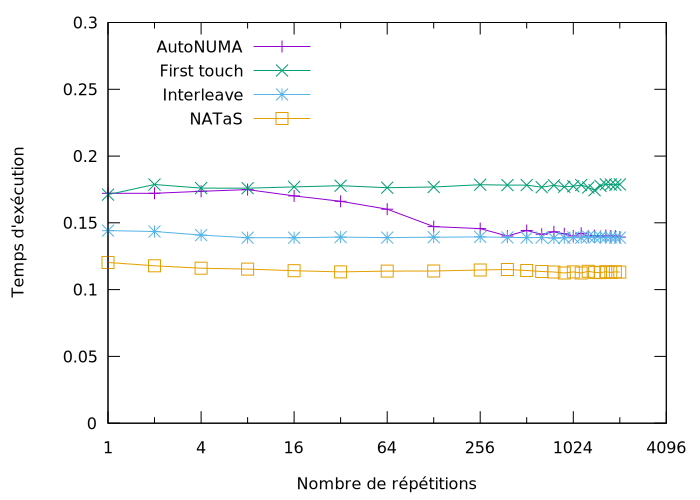
\includegraphics[width=0.7\textwidth]{res_spmv_frep}
  \caption{Temps d'un produit matrice vecteur creux sur Linux 3.18 en mémoire partagée avec 12 coeurs. Nous utilisons une matrice représentant un cube 100 avec 8 variables primaires.}
  \label{fig:res_spmv_frep}
\end{figure}

Avec un nombre de répétitions faibles, AutoNUMA donne les mêmes performances que l'allocation first touch (Fig.~\ref{fig:res_spmv_frep}).
%
Au bout de 8 répétitions, soit environ 1,36~seconde, nous commençons à voir une amélioration des performances.
%
Vers 384 répétitions, soit environ 1 minute, nous obtenons la performance crête d'AutoNUMA qui correspond aussi à la performance obtenue avec l'allocation interleave.
%
Il est nécessaire de rappeler que l'allocation interleave donnait de bonnes performances avec l'utilisation de 2 bancs NUMA.
%
Les meilleurs résultats sont obtenus avec NATaS.
%
Il serait aussi intéressant de tester la méthode AutoNUMA sur Manumanu en utilisant plus de 2 bancs NUMA, nous pourrions savoir si les résultats sont meilleurs qu'avec NATaS.
%
Malheureusement, nous nous ne pouvons pas changer le noyau utilisé sur cette machine.

% -------------------------------

%-------------------------------
\subsection{First touch}
results
%-------------------------------
\subsection{Interleave}
results
%-------------------------------
\subsection{\'Equilibrage automatique NUMA}
Les noyaux Linux récents proposent un équilibrage de charge automatique des pages mémoires.
%
Malheureusement, nous ne pouvons pas utiliser les grappes de serveurs à notre disposition pour tester cette fonctionnalité.
%
La version de Linux n'est pas assez récente, la fonctionnalité autoNUMA n'est apparue que dans la version 3.13.
%
\`A la place, nous allons utiliser une machine de bureau contenant deux processeurs Intel Xeon X5660, chaque banc NUMA dispose de 6 coeurs de calculs et de 24~Go de mémoire vive.
%
La version de Linux utilisée est la 3.18.
%

%-------------------------------
\subsection{NATaS}
\`A la différence des autres ordonnanceurs, NATaS va tenir compte de l'affinité NUMA des tâches.
%
Cette affinité a été définit par Taggre de tel sorte à équilibrer la charge sur les différents banc NUMA.
%



Sur plusieurs bancs NUMA, NATaS offre des meilleurs performances que l'ordonnanceur OpenMP même avec l'allocation mémoire interleaved.
%
{\em Donner résultat manumanu}
%

%-------------------------------
\subsection{Discussion}
Les effets NUMA sont vraiment importants dans le cas d'une application limitée par la bande passante mémoire.
%
Une mauvaise distribution des pages mémoires peut conduire à une sous-exploitation de la bande passante.
%
La politique d'allocation interleaved limite ce problème, on est sûr que tous les liens mémoires sont utilisés, mais on n'a aucun contrôle sur l'amélioration de la localité des accès mémoire.
%
Malgré cela, on obtient un gain important de performance dans certains cas tels que le produit matrice vecteur creux et la résolution triangulaire.
%
Les politiques d'allocations du type next-touch et autoNUMA résolvent une bonne partie du problème en améliorant la localité mémoire.
%
Mais ces politiques ne nous permettent pas d'avoir un contrôle fin de l'accès aux données d'un thread.

La gestion des affinités NUMA directement dans l'ordonnanceur de tâches, nous permet de mieux répartir la charge mémoire.
%
La localité mémoire en devient meilleure et une bonne distribution des tâches donne de très bonnes performances.
%
L'utilisation d'un seul banc NUMA nous montre que l'ordonnanceur NATaS est moins bon que l'ordonnanceur Intel OpenMP.
%
Sur un nombre important de bancs NUMA, NATaS ne passe pas à l'échelle.
%
Cet ordonnanceur a été écrit spécifiquement pour des machines à 2 bancs NUMA.
%
Les gains que nous observons avec l'utilisation de plusieurs bancs NUMA sont bien dus à une amélioration de la localité mémoire.

Malgré les bonnes performances que nous offre NATaS, on pourrait se demander s'il s'agit de la meilleure solution.
%
En effet, le placement des tâches n'est pas optimal, de même que l'équilibrage de charge.
%
Avec les algorithmes actuels, il est impossible de supprimer complètement les accès distants, nous ne pouvons que les limiter.
%
Seule la solution utilisant un processus MPI par noeud NUMA permettrait de supprimer les accès distants.
%
Mais cette suppression se ferait au prix d'un algorithme moins efficace.
%
Donc une meilleure solution pourrait être d'améliorer les ordonnanceurs existants en leur ajoutant une meilleure prise en charge des architectures NUMA.

%   (-_-)   %
\begin{center}
  \begin{tabular}{|r|r|c|c|c|}
    \hline
       & & Cube 100 & Cube 100 & Cube 100 \\
       & & Npri 1   & Npri 3   & Npri 8 \\
    \hline
&        First Touch & 1.91 & 2.18 & 2.49 \\
SpMV &   Interleave  & 2.42 & 2.70 & 3.00 \\
&        NATaS       & 2.08 & 3.08 & 3.80 \\
&        MPI         & 2.89 & 3.29 & 3.81 \\
    \hline
&        First Touch & 5.97 & 6.39 & 8.64 \\
Facto &  Interleave  & 5.50 & 5.62 & 7.51 \\
&        NATaS       & 6.14 & 7.54 & 10.56 \\
&        MPI         & 6.37 & 7.58 & 9.92 \\
    \hline
&        First Touch & 1.69 & 2.12 & 2.71 \\
TRSV &   Interleave  & 1.84 & 2.18 & 2.83 \\
&        NATaS       & 1.82 & 2.49 & 3.48 \\
&        MPI         & 3.21 & 3.26 & 3.70 \\
    \hline
  \end{tabular}
  \captionof{table}{Accélérations obtenues en fonction de la politique d'allocation mémoire. La version MPI ne fait pas exactement le même calcul, elle permet juste d'obtenir une indication sur l'accélération maximale que nous pouvons atteindre.}
  \label{tab:rostand_sum}
\end{center}

Sur une machine avec beaucoup de bancs NUMA, l'ordonnanceur NATaS ne passe pas à l'échelle.
%
Sa structure interne n'est pas assez distribuée, l'utilisation de compteurs globaux de tâches est loin d'être optimal.
%
Malgré une implémentation sous-optimale, NATaS offre de meilleures performances que les ordonnanceurs habituels.
%
Il est donc essentiel d'optimiser les accès mémoire des applications limitées par la bande passante mémoire sur la machine NUMA.

%+++++++++++++++++++++++++++++++


%% %=========================================================
%% \chapter{The fork and join syndrome}
%% \minitoc
%% \vspace{1cm}
%% %=========================================================
%% %+++++++++++++++++++++++++++++++
%% %\section{Data dependencies}
%% %-------------------------------
%% %\subsection{Implicit dependencies}
%% %-------------------------------
%% %\subsection{Explicit dependencies}
%% %+++++++++++++++++++++++++++++++


%% %+++++++++++++++++++++++++++++++
%% \section{The fork and join syndrome}
%% %-------------------------------
%% \subsection{How to see it ?}
%%   \begin{itemize}
%%     \item Show that we have too much synchronization (Paje trace)
%%   \end{itemize}
%% %-------------------------------
%% \subsection{Domain decomposition and overlap}
%%   \begin{itemize}
%%     \item Explain what domain decomposition and overlap is
%%   \end{itemize}
%% %+++++++++++++++++++++++++++++++


%% %+++++++++++++++++++++++++++++++
%% \section{Pipeline GMRES steps}
%%   \begin{itemize}
%%     \item explain the solution to merge graph of task
%%   \end{itemize}
%% %+++++++++++++++++++++++++++++++


%% %+++++++++++++++++++++++++++++++
%% \section{Results}
%% %-------------------------------
%% \subsection{Without MPI}
%%   \begin{itemize}
%%     \item Almost no gain because no many sync
%%   \end{itemize}
%% %-------------------------------
%% \subsection{With MPI}
%%   \begin{itemize}
%%     \item Gain when increase number of MPI process
%%   \end{itemize}
%% %-------------------------------
%% \subsection{Discussion}
%% %+++++++++++++++++++++++++++++++




%=========================================================
\chapter{Conclusions and perspectives}
\minitoc
\vspace{1cm}
%=========================================================
%+++++++++++++++++++++++++++++++
\section{Conclusion}
  \begin{itemize}
    \item Coarsening allow us to parallelize problems with very small computation per task
    \item Improve bandwidth thanks to NUMA architecture
  \end{itemize}
%+++++++++++++++++++++++++++++++


%+++++++++++++++++++++++++++++++
\section{Perspectives}
  \begin{itemize}
    \item Automatic coarse tuning
  \end{itemize}
%+++++++++++++++++++++++++++++++



\backmatter % book mode only
%\bibliographystyle{alpha}
\appendix

\bibliographystyle{annotate}
\bibliography{thesis}
\end{document}
